
\documentclass[sigconf]{acmart}


\usepackage{booktabs} % For formal tables
\usepackage[ruled,vlined]{algorithm2e}
\usepackage{amsmath}
\usepackage{wrapfig} 
\usepackage{balance}
\usepackage{enumitem}
\usepackage{moresize}
\usepackage{subcaption}
\usepackage{epstopdf}
\usepackage{graphicx} 
%\usepackage{geometry}
\usepackage{marginnote}
\usepackage{color}

% \usepackage{pslatex}
\usepackage{multirow} 

\usepackage{enumitem}
\usepackage{bm}
\usepackage{balance}

\newcommand{\newtext}[1]{{\color{blue} #1}}
\newcommand{\margincomment}[1]{\marginnote{{[{\sf {\color{red}\scriptsize #1}}]}}}
\newcommand{\Margincomment}[1]{\marginnote{{[{\sf {\color{blue}\scriptsize #1}}]}}}


\definecolor{myGreen}{rgb}{0.31, 0.78, 0.47}
\definecolor{myRed}{rgb}{0.73, 0.31, 0.28}
\definecolor{myBlue}{rgb}{0, 0.44, 1}
\definecolor{myGrey}{rgb}{0.57, 0.64, 0.69}

\usepackage{array}
\newcommand{\PreserveBackslash}[1]{\let\temp=\\#1\let\\=\temp}
\newcolumntype{C}[1]{>{\PreserveBackslash\centering}p{#1}}
\newcolumntype{R}[1]{>{\PreserveBackslash\raggedleft}p{#1}}
\newcolumntype{L}[1]{>{\PreserveBackslash\raggedright}p{#1}}

%\newcommand\comment[1]{[\textcolor{red}{#1}]
\newcommand\Paragraph[1]{\vspace{0.02in}  \noindent \textbf{#1.}}
\newcommand\Paragraphq[1]{\vspace{0.02in}  \noindent \textbf{#1?}}
\newcommand\Paragraphno[1]{\vspace{0.02in}  \noindent \textbf{#1}}
\newcommand\Textcolor[2]{\hspace*{-3mm} \textcolor{#1}{#2} }

\newcommand{\shubham}[1]{\textcolor{myGreen}{#1}}
\newcommand{\manos}[1]{\textcolor{myRed}{#1}}
\newcommand{\subhadeep}[1]{\textcolor{myBlue}{#1}}


% \AtBeginDocument{%
%   \providecommand\BibTeX{{%
%     Bib\TeX}}}

% \setcopyright{acmcopyright}
% \copyrightyear{2018}
% \acmYear{2018}
% \acmDOI{XXXXXXX.XXXXXXX}

% \acmConference[Conference acronym 'XX]{Make sure to enter the correct
%   conference title from your rights confirmation emai}{June 03--05,
%   2018}{Woodstock, NY}
  
% \acmPrice{15.00}
% \acmISBN{978-1-4503-XXXX-X/18/06}


\begin{document}


\title{Query-driven compaction in LSM-trees}

\author{Shubham Kaushik}
\affiliation{%
    \institution{Boston University}
    \country{USA}
}

\author{****}
\affiliation{%
    \institution{Boston University}
    \country{USA}
}

\author{****}
\affiliation{%
    \institution{Boston University}
    \country{USA}
}

% \author{Ben Trovato}
% \authornote{Both authors contributed equally to this research.}
% \email{trovato@corporation.com}
% \orcid{1234-5678-9012}
% \author{G.K.M. Tobin}
% \authornotemark[1]
% \email{webmaster@marysville-ohio.com}
% \affiliation{%
%   \institution{Institute for Clarity in Documentation}
%   \streetaddress{P.O. Box 1212}
%   \city{Dublin}
%   \state{Ohio}
%   \country{USA}
%   \postcode{43017-6221}
% }

% \author{Lars Th{\o}rv{\"a}ld}
% \affiliation{%
%   \institution{The Th{\o}rv{\"a}ld Group}
%   \streetaddress{1 Th{\o}rv{\"a}ld Circle}
%   \city{Hekla}
%   \country{Iceland}}
% \email{larst@affiliation.org}

% \author{Valerie B\'eranger}
% \affiliation{%
%   \institution{Inria Paris-Rocquencourt}
%   \city{Rocquencourt}
%   \country{France}
% }

% \author{Aparna Patel}
% \affiliation{%
%  \institution{Rajiv Gandhi University}
%  \streetaddress{Rono-Hills}
%  \city{Doimukh}
%  \state{Arunachal Pradesh}
%  \country{India}}

% \author{Huifen Chan}
% \affiliation{%
%   \institution{Tsinghua University}
%   \streetaddress{30 Shuangqing Rd}
%   \city{Haidian Qu}
%   \state{Beijing Shi}
%   \country{China}}

% \author{Charles Palmer}
% \affiliation{%
%   \institution{Palmer Research Laboratories}
%   \streetaddress{8600 Datapoint Drive}
%   \city{San Antonio}
%   \state{Texas}
%   \country{USA}
%   \postcode{78229}}
% \email{cpalmer@prl.com}

% \author{John Smith}
% \affiliation{%
%   \institution{The Th{\o}rv{\"a}ld Group}
%   \streetaddress{1 Th{\o}rv{\"a}ld Circle}
%   \city{Hekla}
%   \country{Iceland}}
% \email{jsmith@affiliation.org}

% \author{Julius P. Kumquat}
% \affiliation{%
%   \institution{The Kumquat Consortium}
%   \city{New York}
%   \country{USA}}
% \email{jpkumquat@consortium.net}


% \renewcommand{\shortauthors}{Trovato et al.}


\begin{abstract}
  In modern data systems, particularly for write-intensive workloads, log-structured merge (LSM) trees have become the 
most widely used technique. The idea of out-of-place updates, which logically invalidate keys that may exists on 
multiple levels, helps LSM-trees excel for write heavy workloads. However, current LSM-tree designs do not capitalize on 
the sort-merge operations performed for the range queries, which leads to carrying out almost the same amount of work 
for each range query, even when they are same or overlapping. This inefficiency can result in the wastage of CPU cycles 
and unnecessary I/O operations in worst-case scenarios due to presence of logically invalid keys.

In this paper, we present a query-driven compaction strategy that removes the invalid (logically deleted) keys from the 
LSM-tree and flushes back the valid keys filtered by sort-merge performed during a range query. We conduct performance 
experiments with the help of a custom implementation in one of the popular LSM-based data stores, RocksDB.\
  
\end{abstract}

% \keywords{datasets, neural networks, gaze detection, text tagging}



\maketitle

\section{Introduction}
\label{sec:intro}
\Paragraph{Write heavy workloads with LSM} The rising research in the field of robotics and IoT devices, combined with the 
integration of artificial intelligence and machine learning, has resulted in the generation of vast amounts of data.
This data often requires real-time processing and exhibits a write-heavy nature. The data stores like RocksDB and 
LevelDB have been designed to efficiently handle such workloads. These data stores rely on the technique of
\textbf{log-structured merge (LSM)} trees, an efficient data structure tailored for managing write-heavy workloads. The
fundamental concept underlying LSM trees is of out-of-place updates, which logically invalidate keys instead of 
performing in-place updates.

\Paragraph{Compaction} The LSM trees are composed of multiple levels, each of which is a sorted run of key-value pairs. 
The compactions are performed to merge the sorted runs from the lower levels into the higher levels. The process is 
triggered when the size of a level exceeds a certain threshold. It helps in removing the stale data from LSM and 
making room for new data in lower levels.

\Paragraph{Range queries} The LSM design is optimized for write-heavy workloads, but it also supports range queries. The
range queries are performed by merging the sorted runs from multiple levels and filtering out the keys that have been
logically invalided. This process is also called \textbf{sort-merge}, which is similar to the compaction~\cite{Sarkar2021}.

\Paragraph{Problem} When executing a range query, the sort-merge operation is performed on sorted runs from multiple 
levels that retrieves both valid and invalid keys from those levels. Consequently, more data is read than 
actually required. This situation is acceptable when performing a single range query for a specific range. However, when 
the same query or an overlapping one is executed repeatedly, a nearly identical amount of work is executed. Furthermore, 
when a compaction is triggered within that specific range, some of the invalid keys that were previously read, sorted 
and filtered during the range query are revisited. This results in redundant CPU cycles and I/O operations, where the 
same data bytes are read repetitively until reaching the last level.


% Motivation
\subsection{Motivation}
The repetition of work involving invalid keys can be effectively mitigated by redirecting valid keys, filtered through 
the sort-merge operation during a range query, back to the higher levels. This approach can be termed as 
\textbf{query-driven compaction}. By minimizing the presence of invalid keys within the LSM tree, the compaction process 
gains efficiency, subsequently leading to less number of I/O operations and a more optimal utilization of CPU cycles.


% Problem Statement
\subsection{Problem Statement}
The state-of-the-art LSM-based data stores performs range queries by retrieving multiple files from various levels and 
filter out invalid keys. Once the range query is complete, the work done by the sort-merge operation for the query is 
discarded. The results are neither cached nor flushed back to the LSM tree except just returning it to the application. This 
approach can give rise to two problems: (1) \textit{Redundant Work}: when the same range query or 
an overlapping one is executed again, and (2) \textit{Increased Write Amplification}: when a compaction is triggered 
for the files containing invalid keys or keys that were accessed within the last few range queries. During these process, 
the system re-reads the invalid keys and subsequently either drops them or replaces them with new values. As a result, 
the same data bytes are read and written during both the range query and compaction processes, leading to higher read, 
write, and space amplification.


% Contributions
\subsection{Contributions}
In this paper, we present a query-driven compaction strategy that involves writing the valid keys back to the higher 
levels of the LSM tree. While this approach may slightly increase the flush write bytes during a range query, it 
substantially reduces the presence of invalid keys in the LSM tree. As a result, there is a notable reduction in read, 
write, and space amplification during both compaction processes and future range queries. We have also implemented our
approach in RocksDB, a popular LSM-based data store and conducted a series of experiments to evaluate its performance.
The contributions impacting different parameters are as follows.

\Paragraph{Reduced Space Amplification}
The Range Query-Driven Compaction (RQDC) approach exhibits a significant reduction in space amplification compared to 
the vanilla approach. In a workload scenario consisting of an initial epoch with 1 million inserts followed by 10 
epochs, each involving 250,000 updates and 10 interleaved range queries of 10\% selectivity (size ratio 4 and entry size of 256 bytes), 
shows some notable findings. Specifically, employing RQDC with lower and upper bounds set at 0.25 and 1.5, 
respectively, resulted in a 4\% reduction in space usage than vanilla. Additionally, a more aggressive setting with lower and upper 
bounds set at 0 and 6, respectively, showed a substantial 14\% decrease in space utilization. The reduction in space 
amplification is attributed to the elimination of invalid keys during query-driven compactions, leading to a more 
space-efficient storage structure. This lower and upper bound decide how big the compaction it can perform, when it is set
to 0 and 6, it compact more data for a specific range query than it does for 0.25 and 1.5.

\begin{figure}
    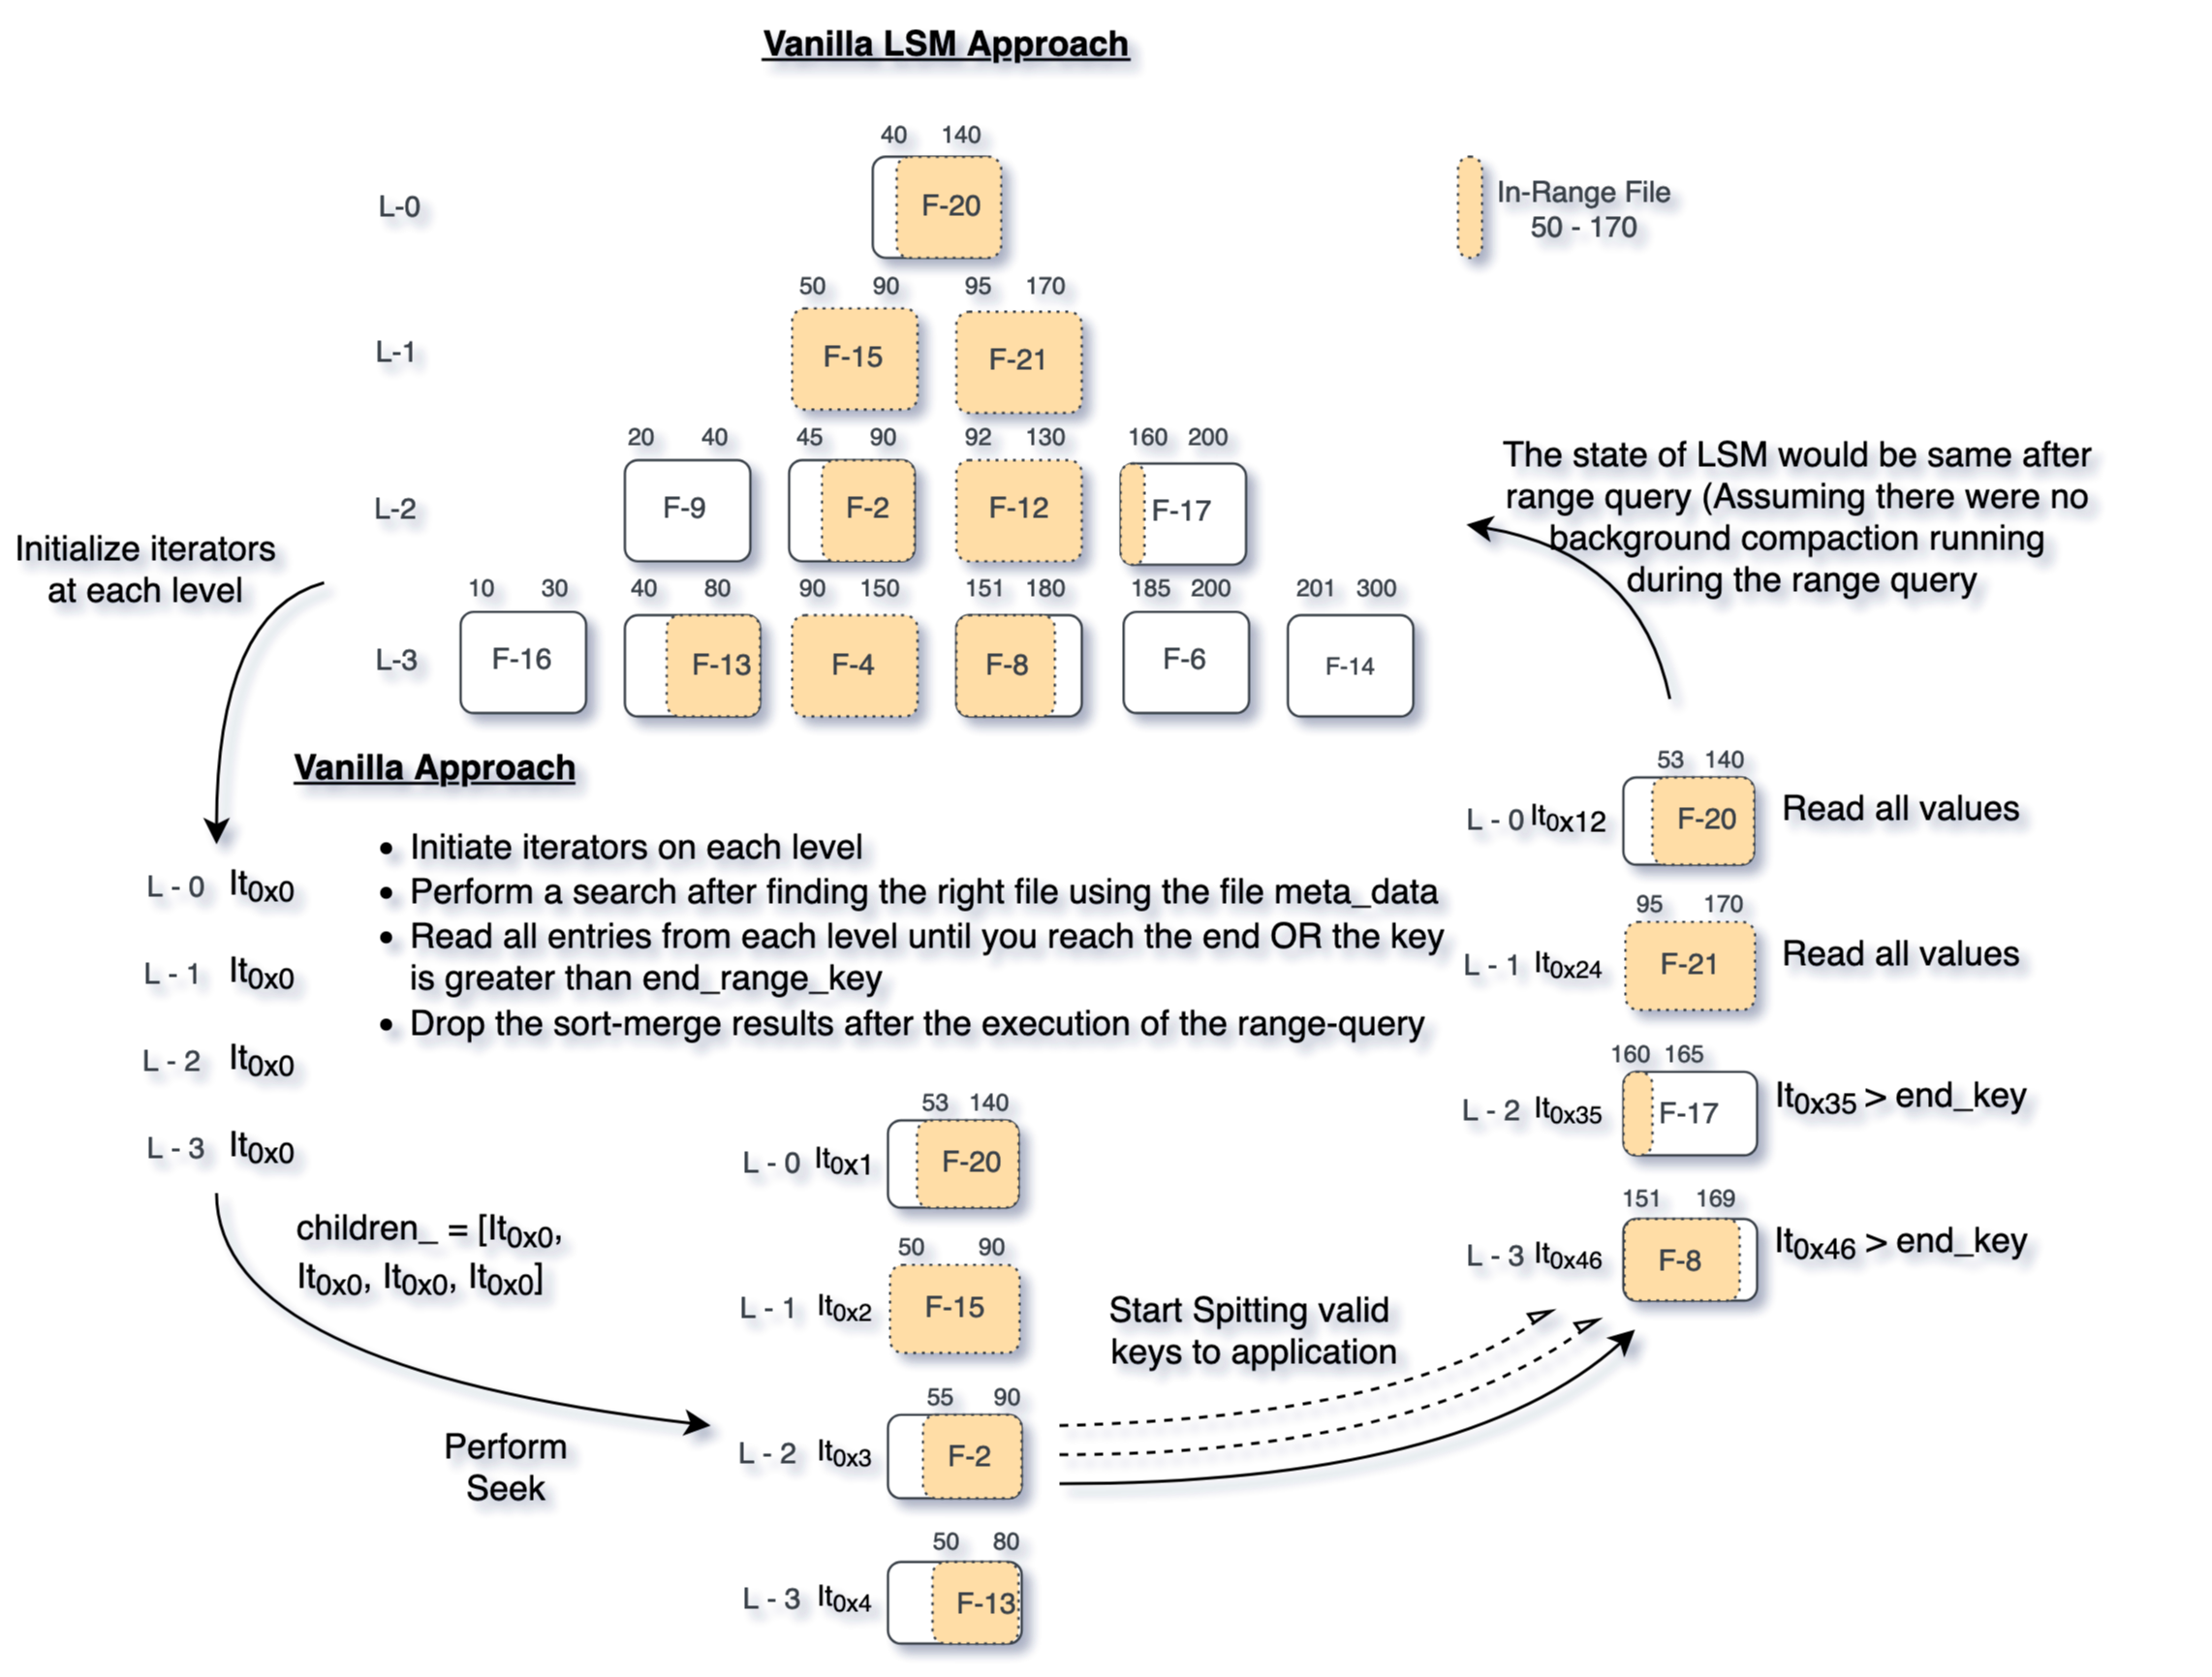
\includegraphics[scale=0.11]{Figures/Vanilla Range Query vanilla.png}
    \caption{Flow of ``vanilla'' range query in LSM. This outlines the sequential steps involved in a range 
    query}\label{fig:vanilla_range_query}
\end{figure}

\Paragraph{Improved Range Query Performance}
RQDC significantly enhances the efficiency of range queries, as evidenced by findings from a workload scenario same as 
above. In the vanilla approach, there was a continuous increase in the 
percentage of invalid keys read by range queries (show in Figure~\ref{fig:increased_invalid_keys}), reaching up to 2\% of unique inserts by the end of the workload run. 
However, when the experiment was conducted with RQDC, specifically with lower and upper bounds set at 0 and 6, 
respectively, the percentage of invalid keys read by range queries came down to 0.7\% with a cost of a 30\% increase in 
average range query time (shown in Figure~\ref{fig:reduced_invalid_keys} and Figure~\ref{fig:increased_range_queries_time}). 
While there was a maximum spike of 0.7\% in the invalid keys read by 4 out of 100 range 
queries, the remaining 96\% of range queries read less than 0.5\% of invalid keys. We ran the same experiment with the 
lower and upper bound set to 0.25 and 1.5 with RQDC, showing a 1.1\% of invalid keys at the end of the experiment, 
which is lower than vanilla at a cost of a 2\% increase in average range query time (shown in Figure~\ref{fig:another_epoch_with_lb_ub} and Figure\ref{fig:range_queries_time}).

\Paragraph{Optimized Write Amplification}
While RQDC introduces additional writes during the query-driven compaction process, it maintains a competitive write 
amplification level similar to the vanilla approach using configurable lower bound and upper bound thresholds. The 
experiments that we ran for the same epoch workload showed that for the lower and upper bound of 0 and 6, the 
write amplification increases up to 5\% compared to vanilla, and for the lower and upper bound of 0.25 and 1.5, it
goes to 8\%. The strategy of eliminating invalid keys during compactions, triggered by range queries, increases write 
amplification slightly, which can be controlled by changing the values of the lower and upper bound.


\section{Background}
\label{sec:background}
\begin{figure}
    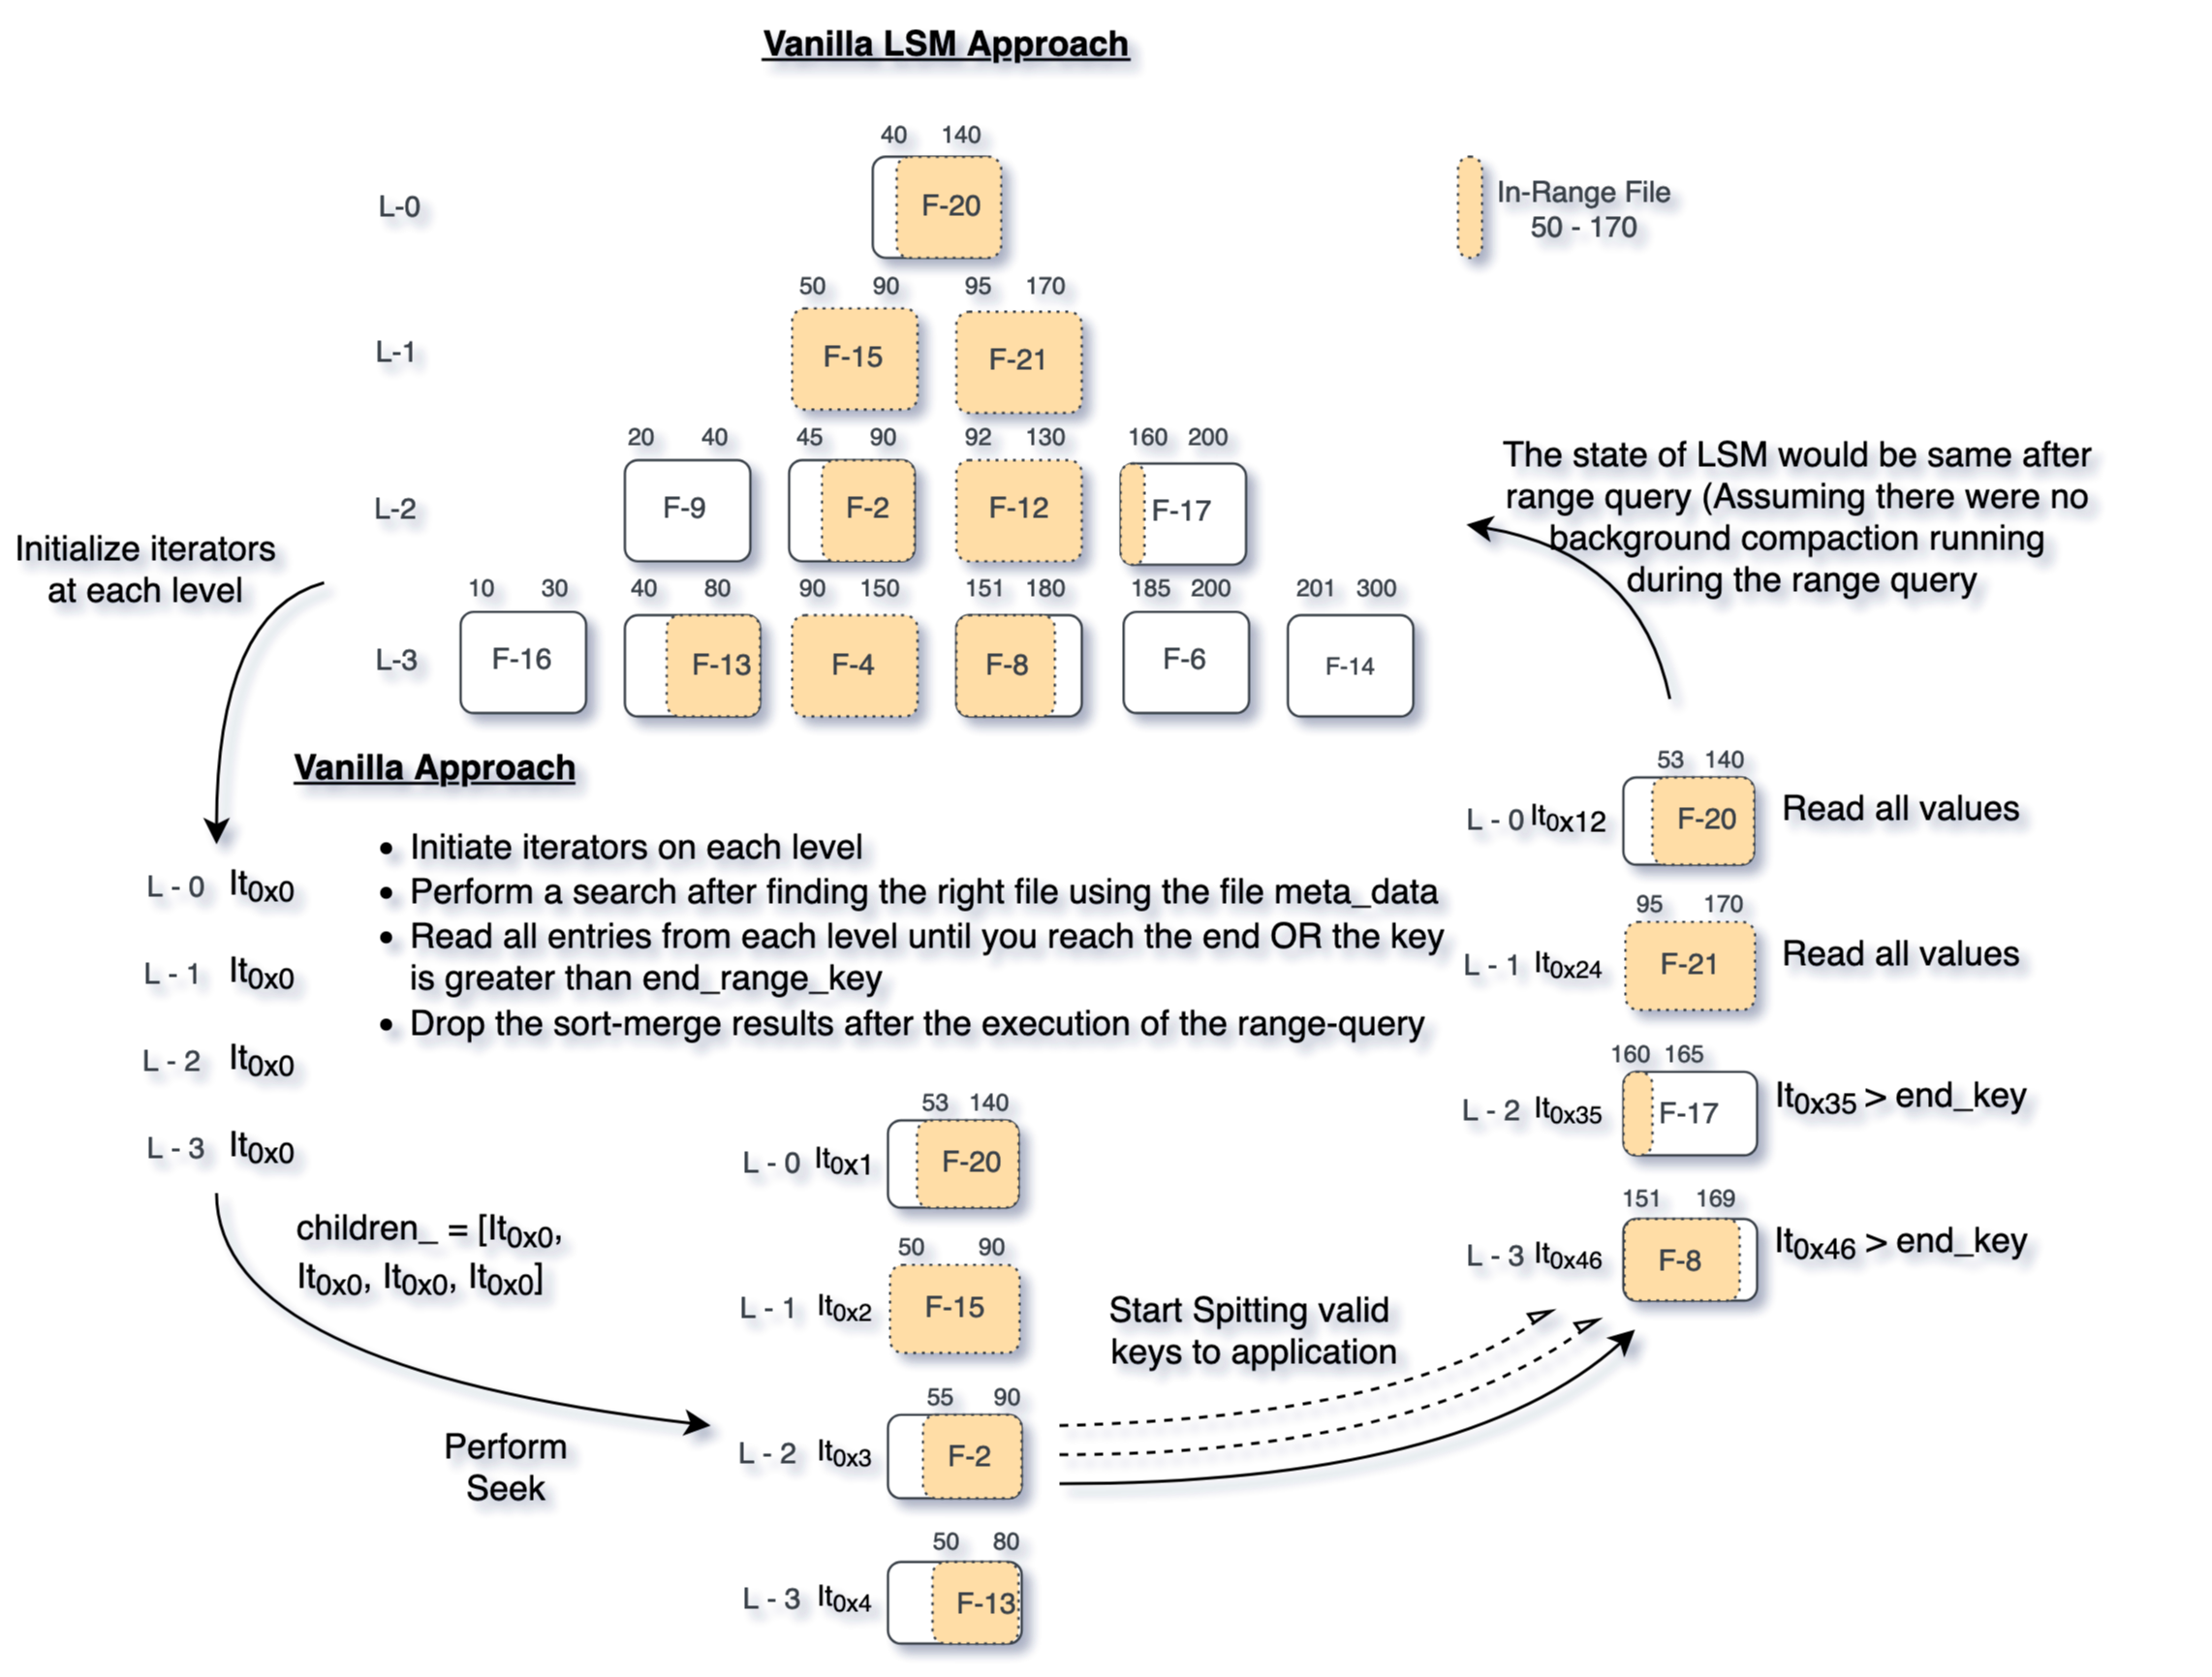
\includegraphics[scale=0.10]{Figures/Vanilla Range Query vanilla.png}
    \caption{Vanilla range query flow in LSM}\label{fig:vanilla_range_query}
\end{figure}

LSM-based data stores are designed to efficiently manage write-heavy workloads. The data is ingested through 
an in-memory buffer (a.k.a memtable in Rocksdb), a data structure that stores keys and their corresponding values. 
Once an in-memory buffer reaches its capacity, it is flushed to the disk in the form of an immutable sorted file (a.k.a Sorted Strings Table, SSTable or SST). 
These sorted files together forms a single sorted run which represents one level of LSM tree. Every level is completely sorted 
across all files, that are sorted by key. The compactions are triggered in the background when the size of a level exceeds a 
specific threshold.

\Paragraph{Updates in LSM} Updates are executed in an out-of-place fashion, where new values are written to lower levels 
while retaining old values in higher levels.

\Paragraph{Deletes in LSM} Deletions are performed by adding a special marker called a \textit{tombstone}. Tombstones are 
utilized to filter out logically deleted keys during range queries or compactions. They also serve as a form of soft 
deletion for point queries. Tombstones are removed when they reach the lowest level of the LSM structure.

\Paragraph{Range queries in LSM} LSM supports range queries by merging keys from multiple levels and filtering out 
invalid keys.

In the context of range queries, LSM-based data stores typically employ a straightforward approach: they create an 
iterator for each level and perform a K-way merge. This merge process involves pulling files sequentially or 
asynchronously from each level into memory and executing a sort-merge operation. The K-way merge eliminates the need 
to load all files from each level into memory simultaneously, thus reducing memory footprint.

\Paragraph{Leveled Compaction} Leveled compaction uses ``merge with'' strategy, where each level is merged with 
next level, which is usually much larger as per the configured size ratio.

The compactions are triggered to move data from lower levels to higher levels. The process involves selecting a file 
based on a compaction score from the lower level using a configured compaction policy. This file is then merged with 
overlapping files from the higher level. Invalid keys are filtered out during this merge, and the valid keys are 
written to the higher level. The compaction process will always occurs between adjacent levels. Once a file is compacted, 
it is removed from the lower level, and the new compacted file is written to the higher level. This process can repeat
multiple times until the level size falls below a specified threshold. 


\section{Problem}
\label{sec:design_space}
In the preceding background section, the compaction process (specifically, the Leveled compaction) was discussed, 
highlighting its occurrence between adjacent levels. Now, let's delve into a scenario involving an LSM tree with $N$ 
levels and a set \textit{size ratio} of 10. In this context, the compaction process selects files randomly from lower 
levels based on the configured compaction policy.\\
Let's consider a scenario where each level shares at least one common key across all levels. Now, envision the 
initiation of compaction from the lowest level (level 0) to the highest level, sequentially. In this process, a 
specific key would be read $N$ times and written $N$ times. This repetition arises as the key is initially read from 
level 0 and subsequently written to level 1, then read from level 1 and written to level 2, and so on. This simple 
illustration serves to demonstrate the concept of read and write amplification. However, it's important to recognize 
that in actuality, the compaction process is significantly more intricate, involving multiple files across multiple 
levels. As a result, the read and write amplification is notably higher in complex cases.\\
For a more tangible understanding, consider the ideal scenario where the \textit{size ratio} is 10. In this case, to 
propagate a single byte from the $i^{th}$ level to the $(i+1)^{th}$ level, a maximum of 11 bytes must be read.
Applying this principle to the earlier example, with $N$ levels each containing the same key, we effectively encounter 
the need to read and write 11 bytes a total of $N$ times due to the presence of $N$ levels sharing the common key.
 
\section{Solution Name}
\label{sec:solution}

\begin{figure}
    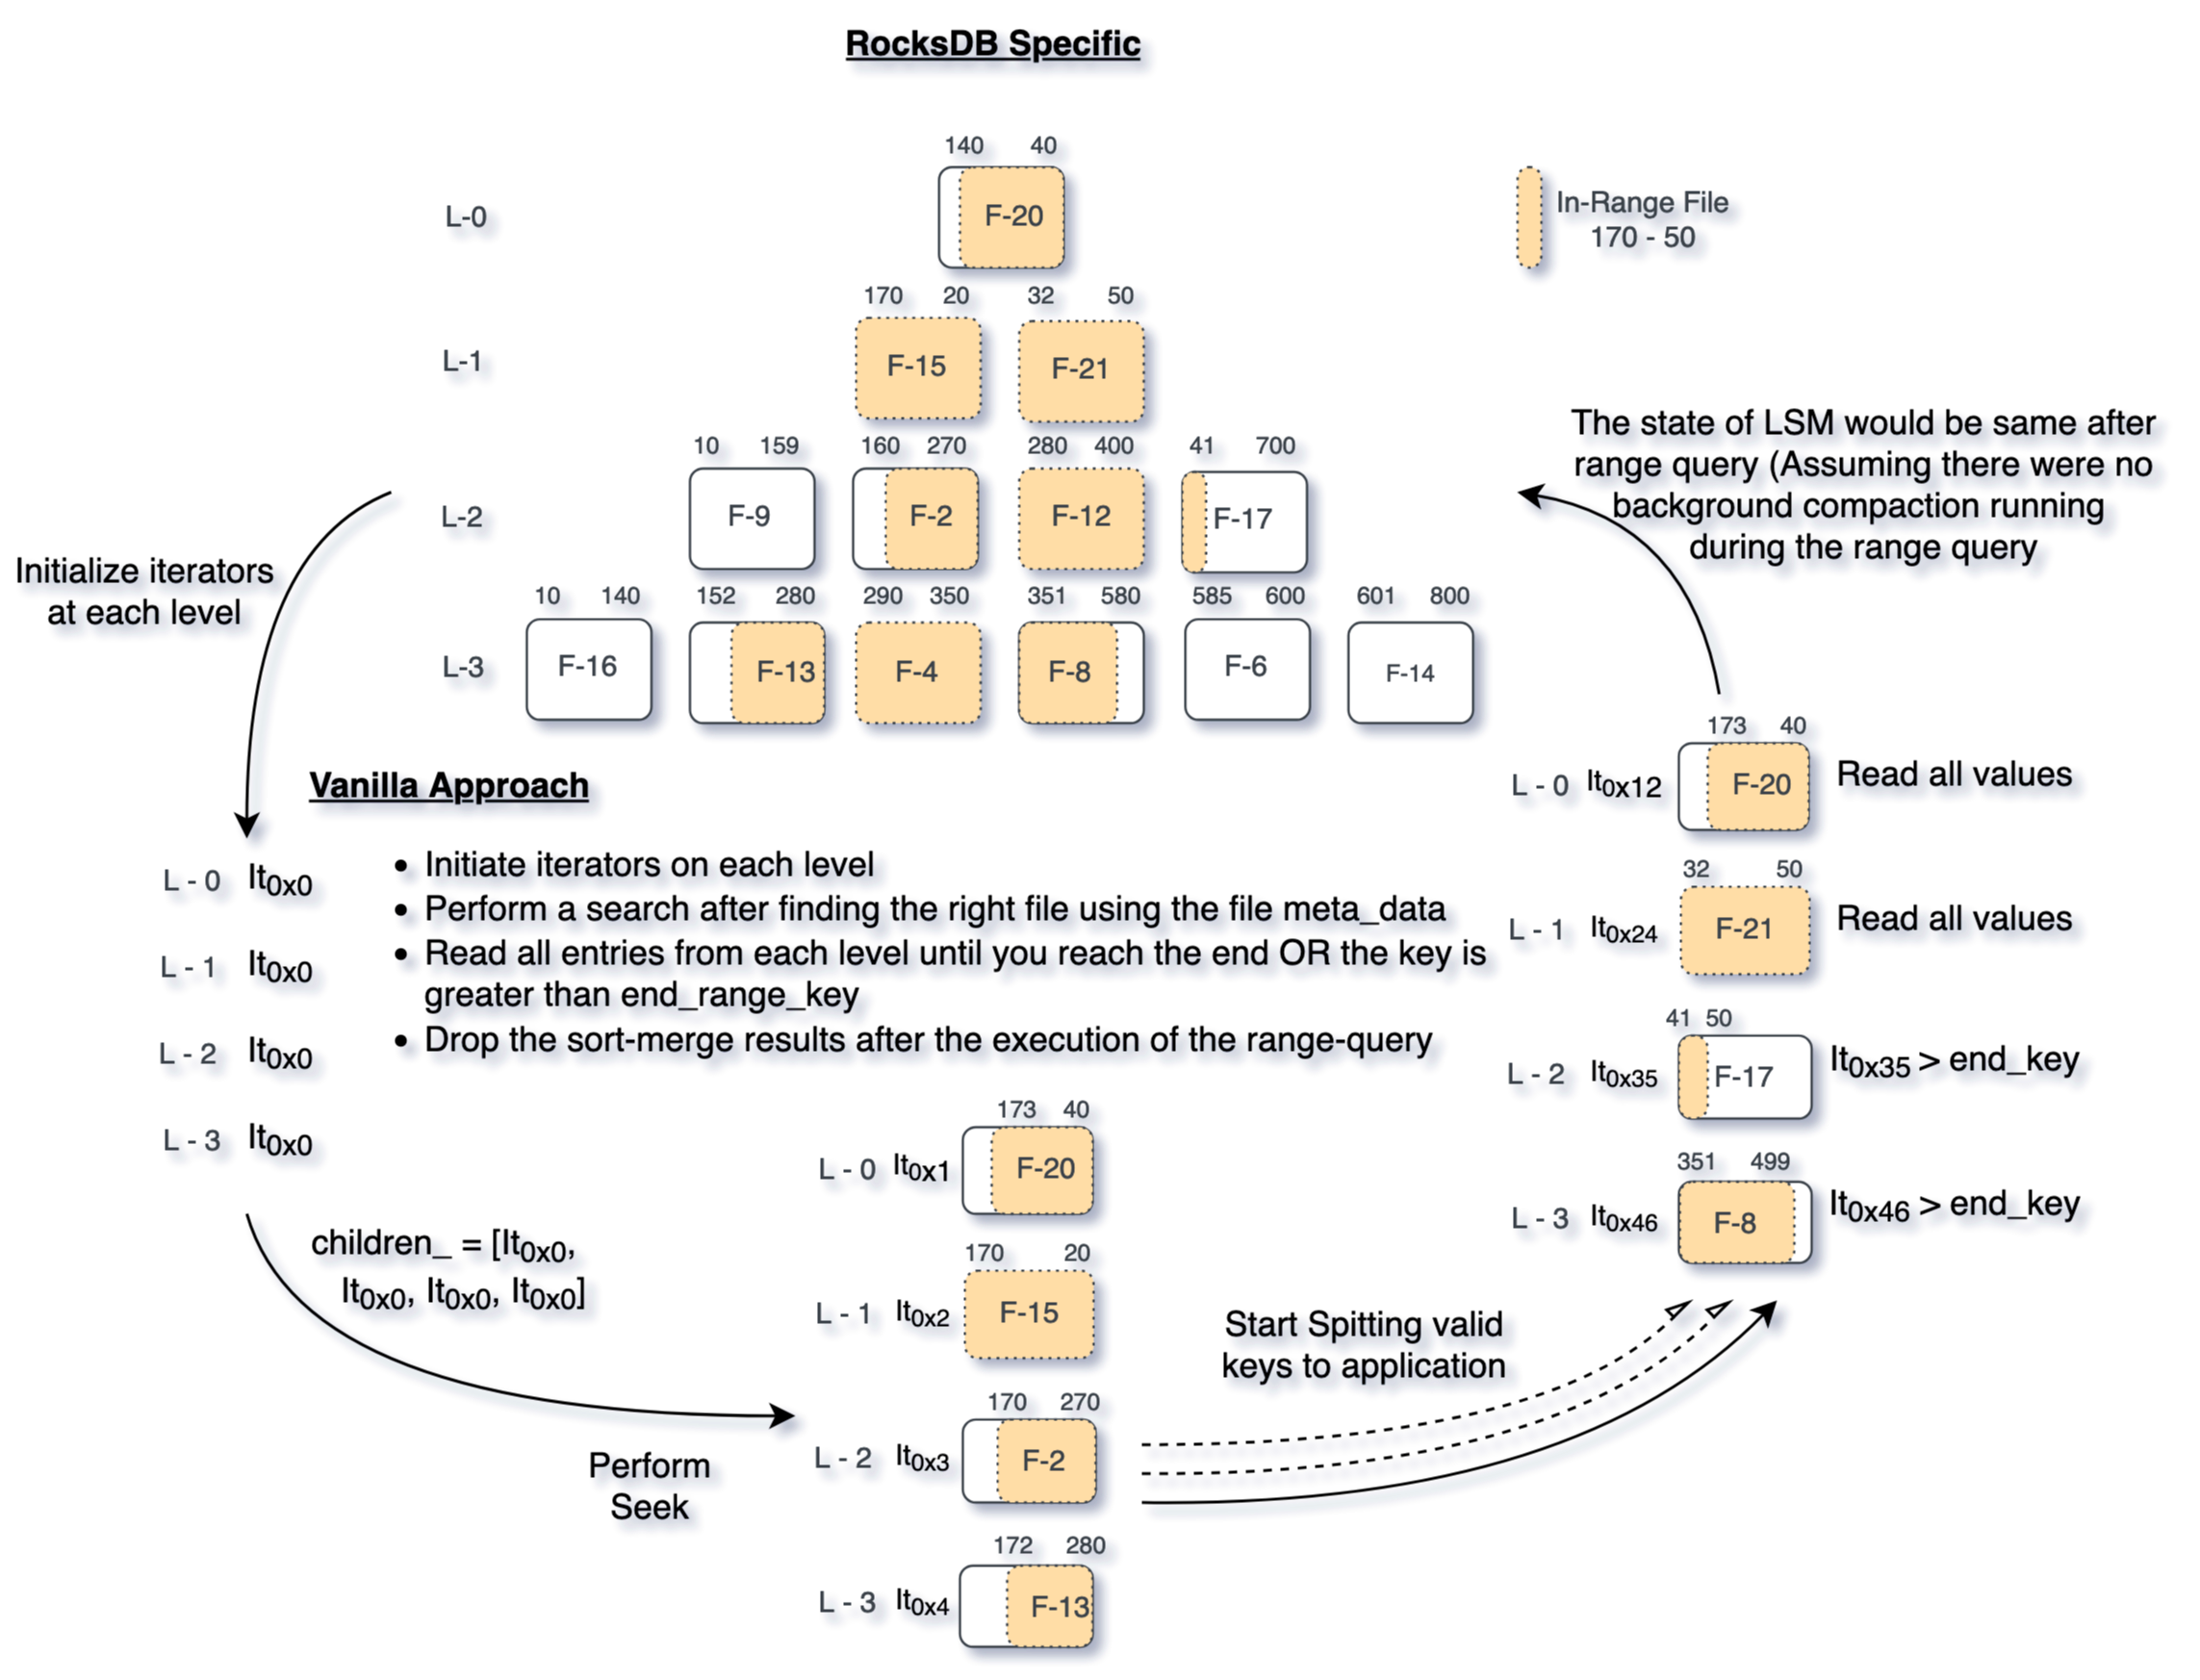
\includegraphics[scale=0.10]{Figures/Vanilla Range Query rocksdb specific.png}
    \caption{Range query flow in lexicographically sorted files}\label{fig:rocksdb_specific_vanilla_range_query}
\end{figure}


\begin{figure*}
    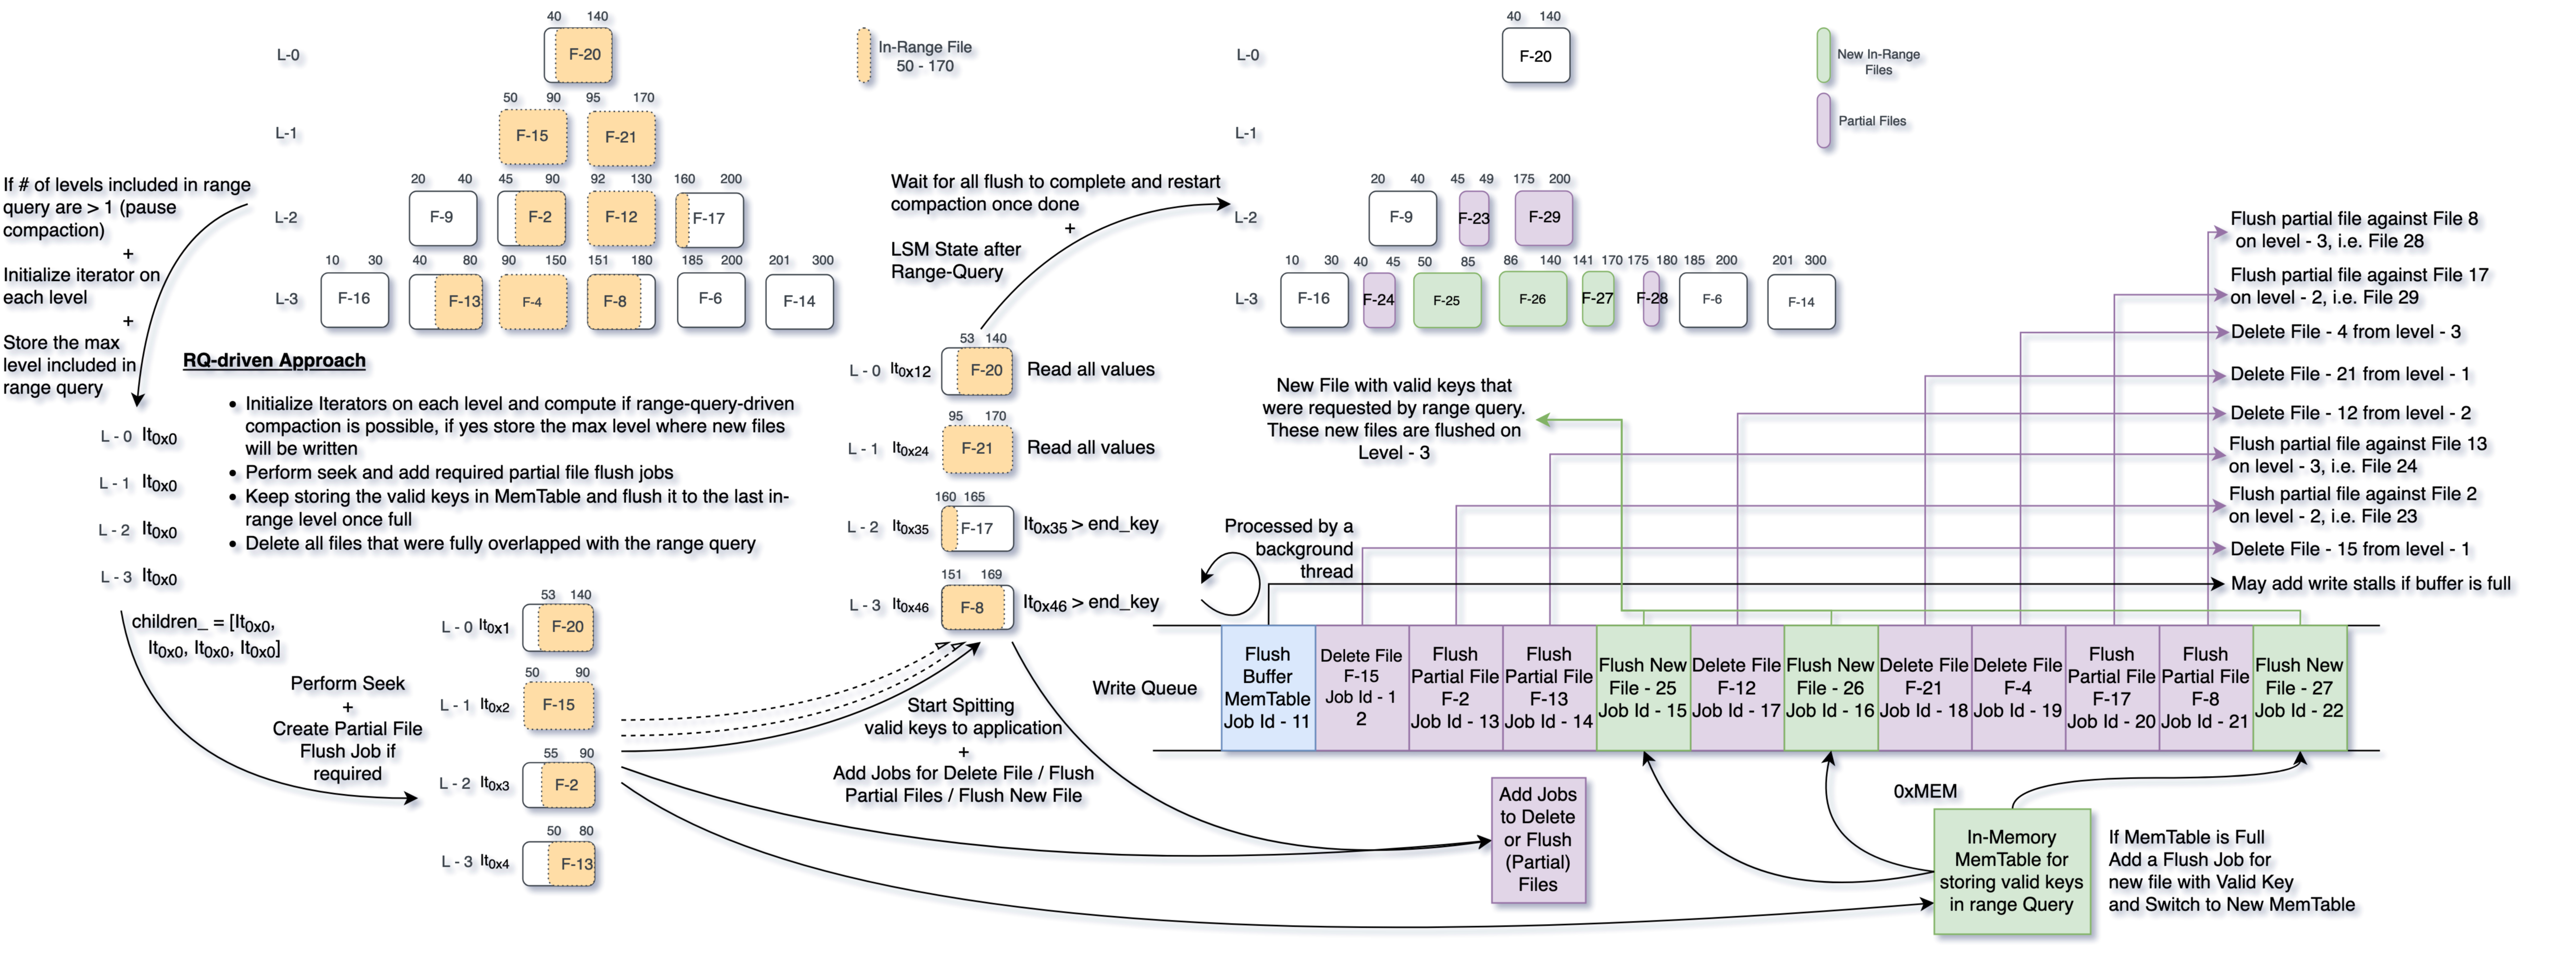
\includegraphics[scale=0.10]{Figures/RQ-driven numeric key sorting.png}
    \caption{Query-driven compaction flow in LSM}\label{fig:query-driven_compaction}
\end{figure*}

\begin{figure}
    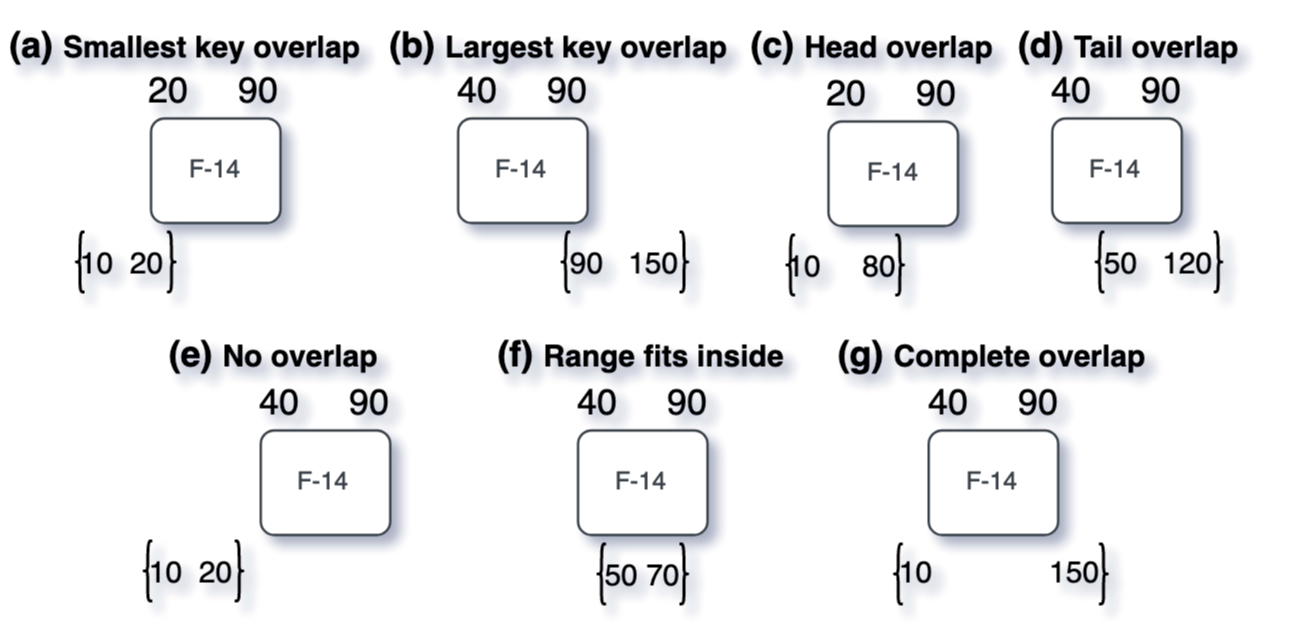
\includegraphics[scale=0.2]{Figures/File range overlaps.png}
    \caption{File range-query overlaps}\label{fig:file_range_overlaps}
\end{figure}

\begin{figure*}
    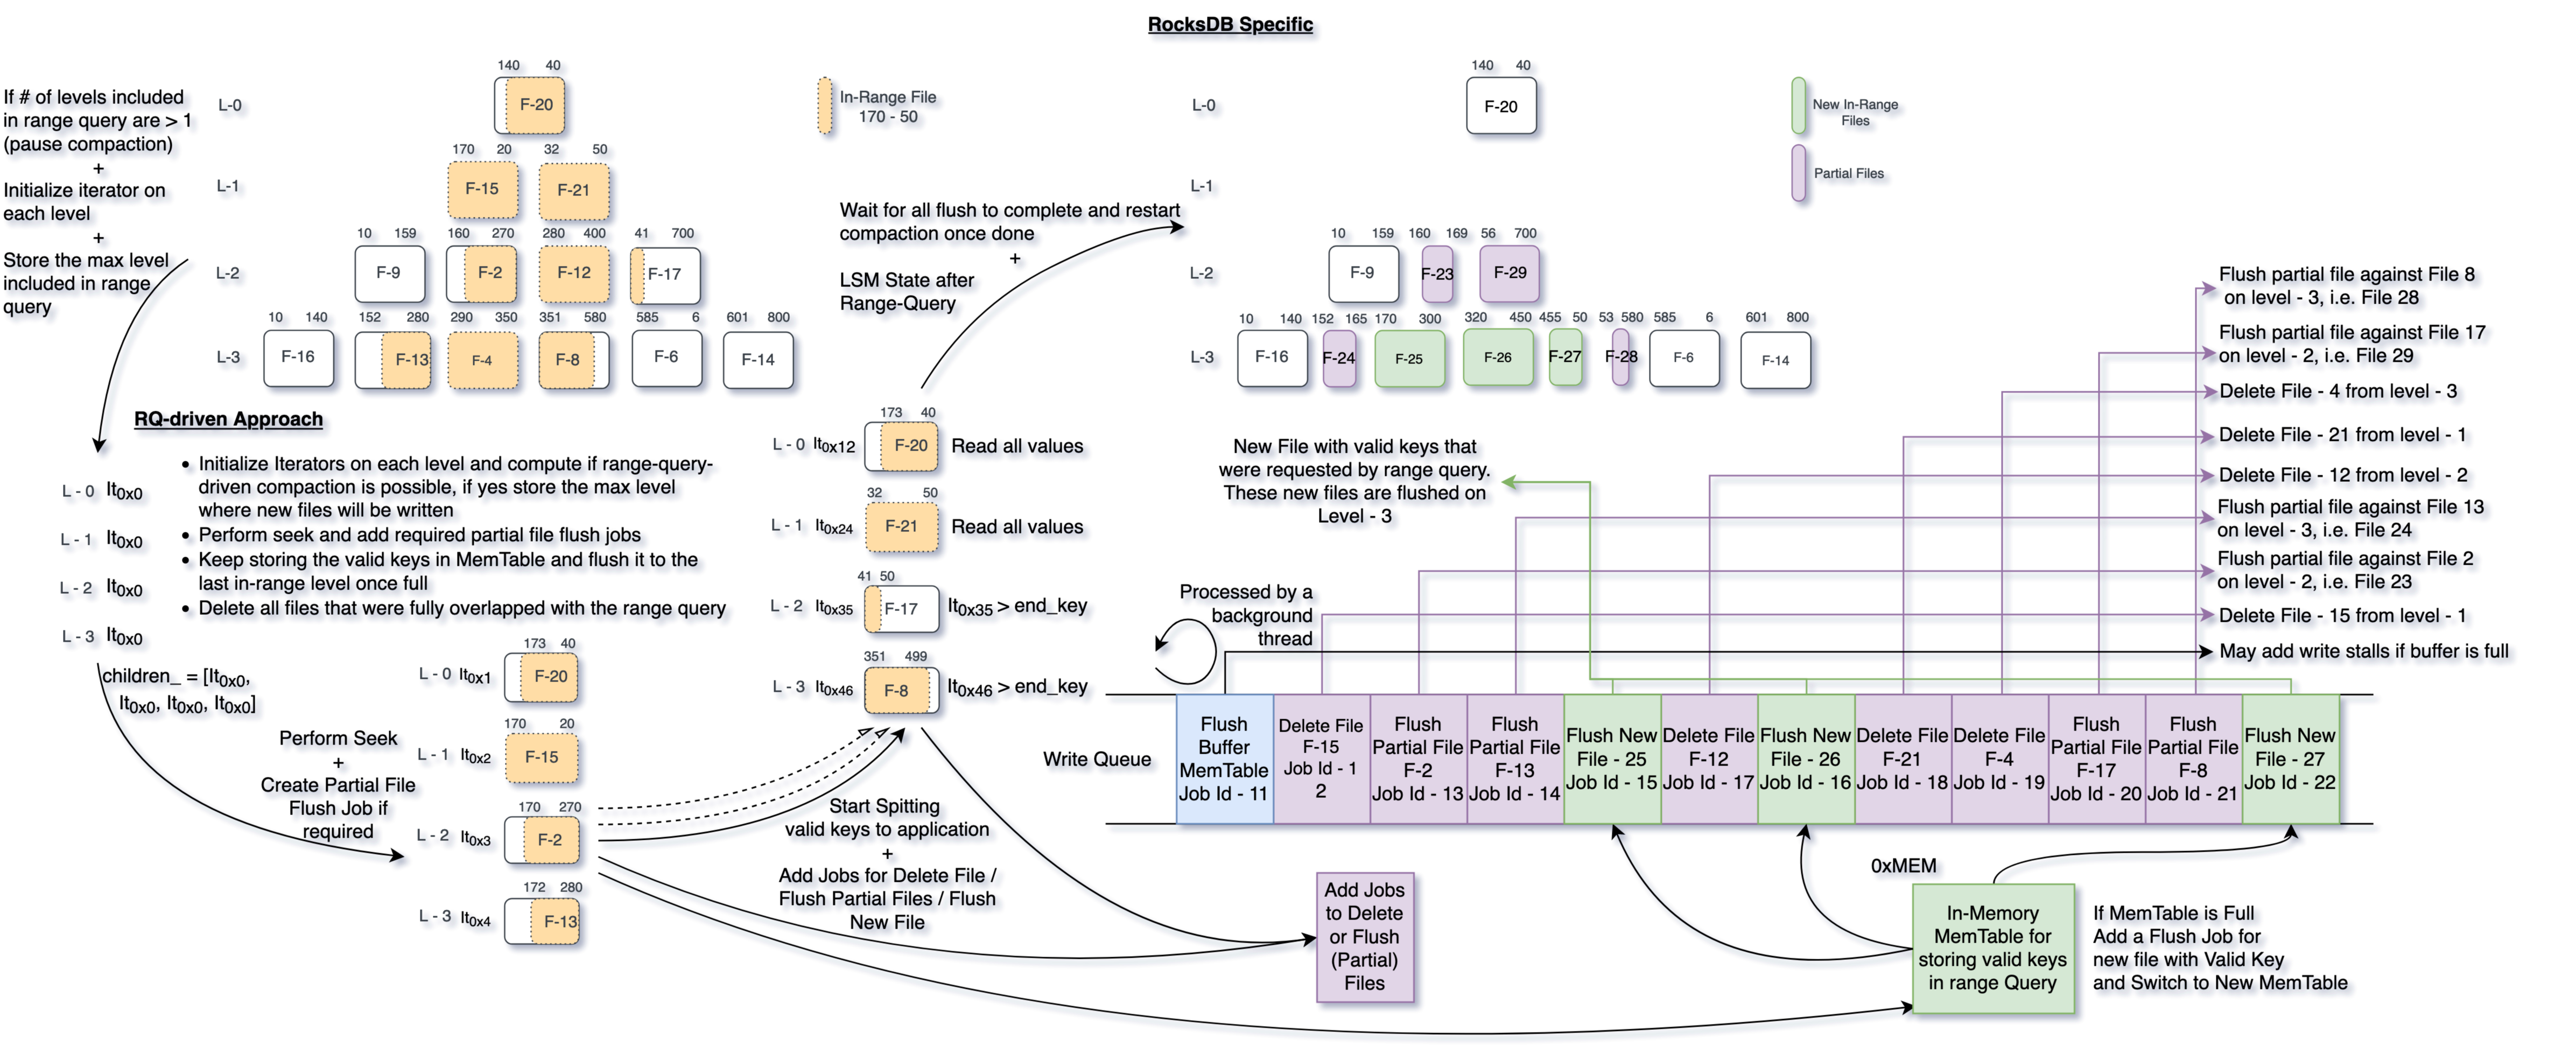
\includegraphics[scale=0.10]{Figures/RQ-driven rocksdb specific.png}
    \caption{Query-driven compaction flow in lexicographically sorted files}\label{fig:rocksdb_specific_query-driven_compaction}
\end{figure*}

The solution to the problem of redundant work and increased write amplification is query-driven compaction. This 
approach involves writing the valid keys back to the higher levels of the LSM tree.

\subsection{Vanilla Approach}
The flow of range query in vanilla approach is shown in Fig-\ref{fig:vanilla_range_query} and 
Fig-\ref{fig:rocksdb_specific_vanilla_range_query}. The query runs by 
initiating the iterators for each level of LSM tree and then perform a seek operation on each iterator to find the 
first key that is greater than or equal to the start key of the range query. It then iterates through the
SSTables in the LSM tree and returns the values that fall within the key range. At the end of the range query
execution the state of LSM tree would be same as before the query execution.

\subsection{Query-driven Compaction}
The flow of range query in query-driven compaction is shown in Fig-\ref{fig:query-driven_compaction} and 
Fig-\ref{fig:rocksdb_specific_query-driven_compaction}. The initial 
setup of level iterators goes the same as in the state-of-the-art LSM range query. Once all the iterators are 
initialized, it performs a seek operation on iterators using the range-query start\_key for each level. The seek 
operation in query-driven compaction performs an extra operation to create a partial file flush job and add it to the 
write\_queue\_. The partial file flush will only happen if the file does not completely overlap with the range-query 
start\_key and end\_key. We can have three scenarios for the partial file flush, which 
(as shown in Fig-\ref{fig:file_range_overlaps}) are as follows.

\begin{figure*}
    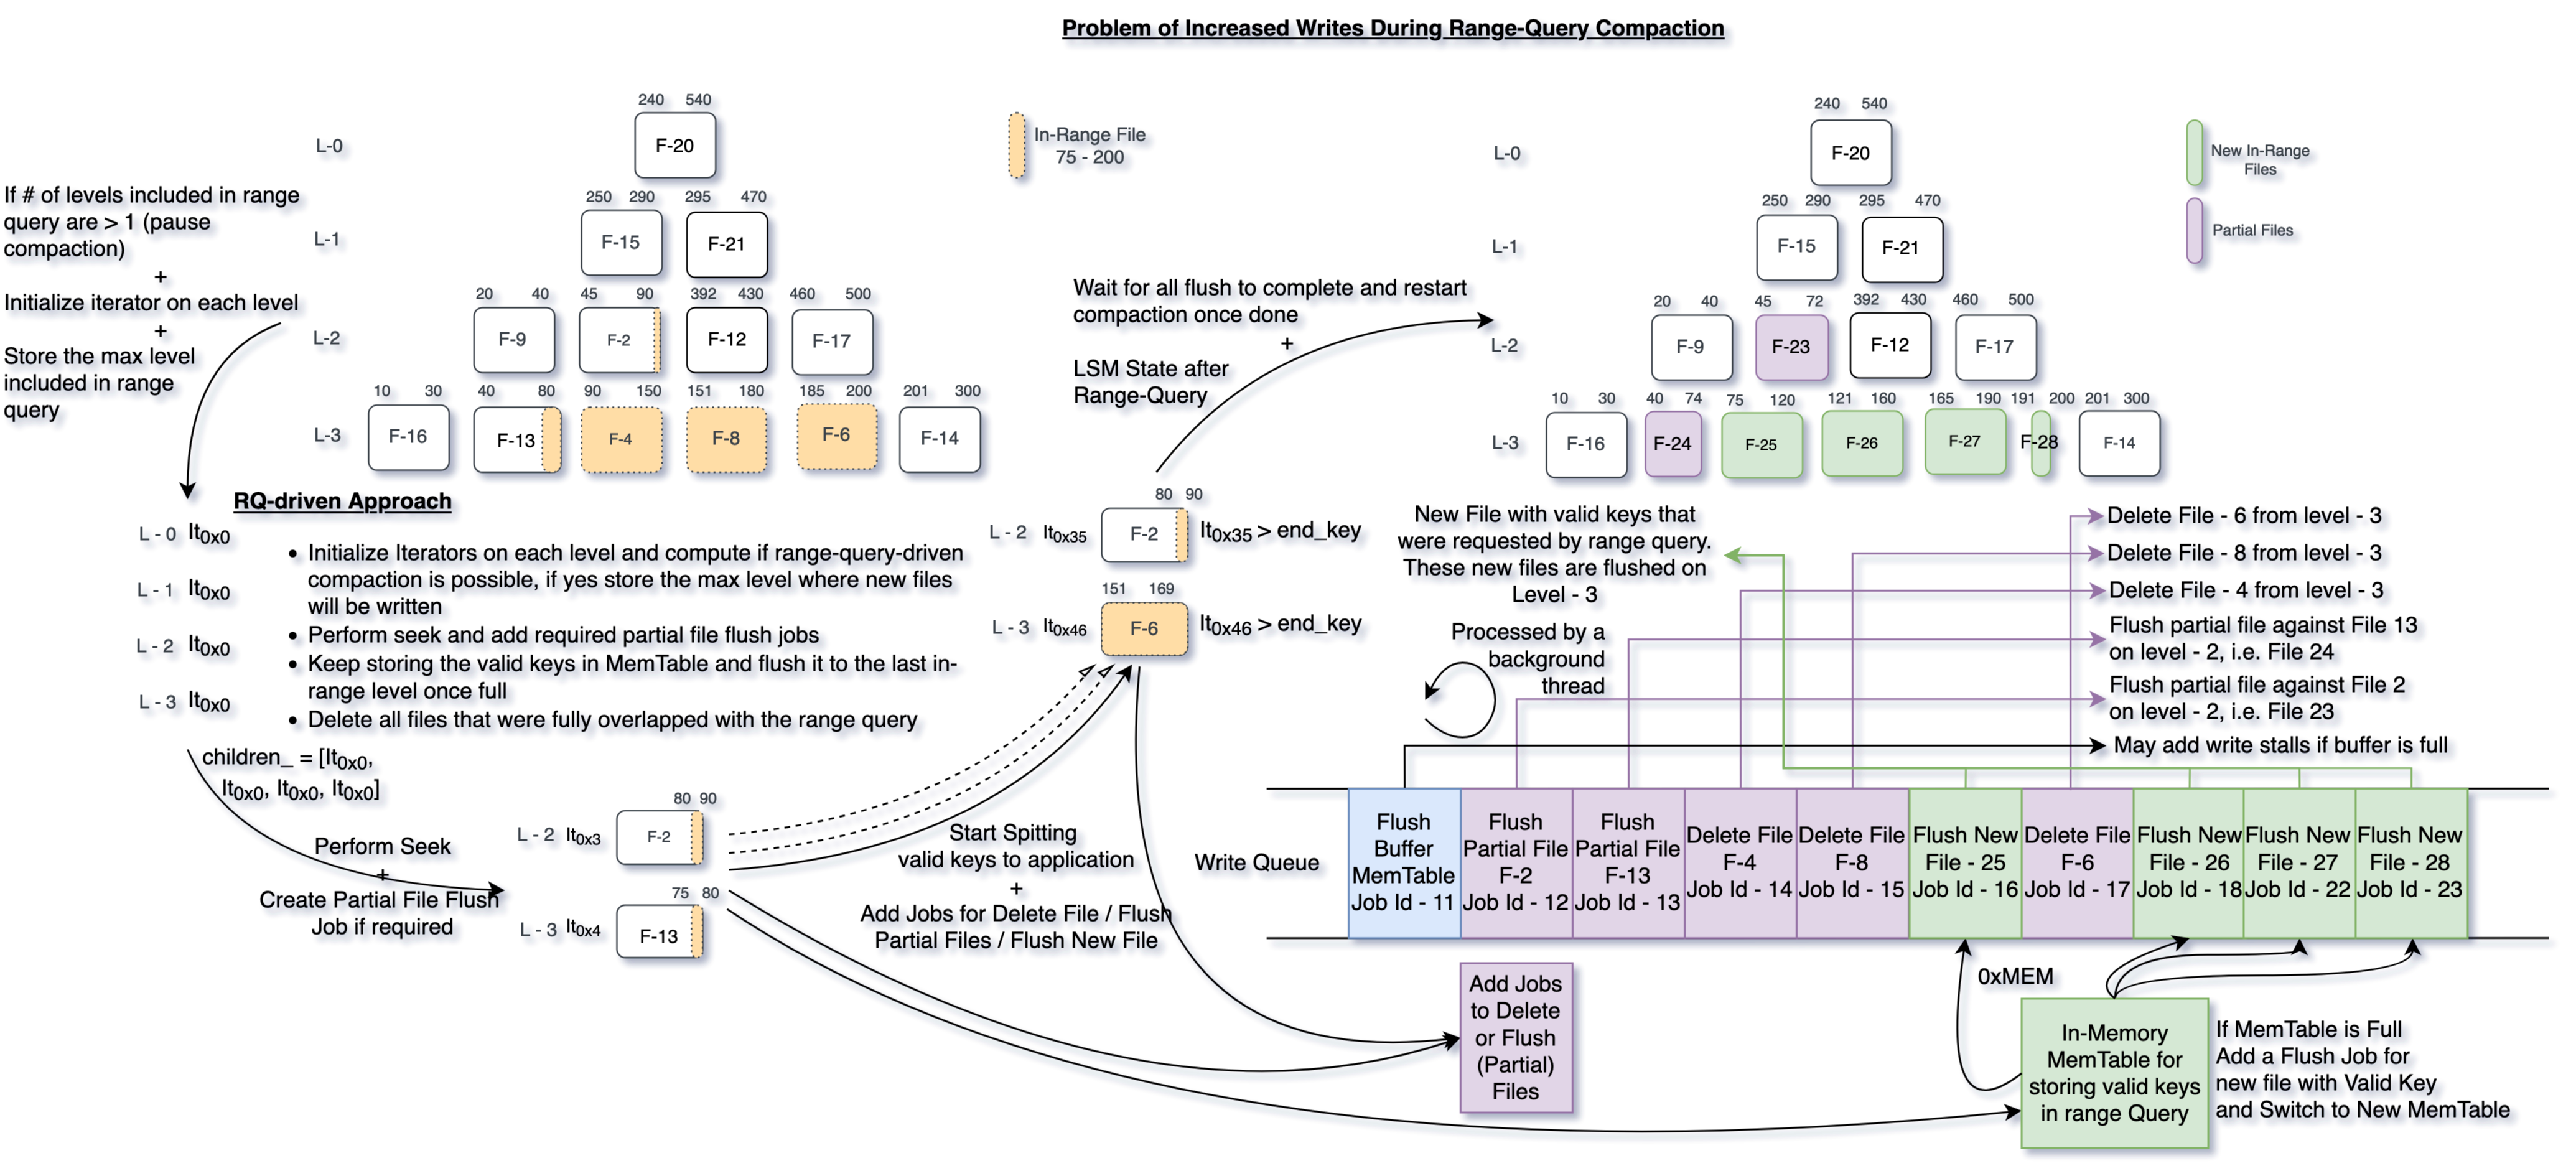
\includegraphics[scale=0.12]{Figures/RQ-driven problem of increased writes.png}
    \caption{Query-driven compaction with increased writes problem due to less overlap}\label{fig:query-driven_compaction_with_increased_writes}
\end{figure*}

\begin{enumerate}
    \item \textbf{No overlap} In this scenario, the partial file flush will not happen as the file does not overlap. 
    Fig-\ref{fig:file_range_overlaps} (e)
    \item \textbf{Smallest or Largest key overlap \textit{(Partial Flush)}} In this, the smallest or largest key of the 
    file overlaps with the range query start or end key. Fig-\ref{fig:file_range_overlaps} (a) and (b)
    \item \textbf{Head or Tail overlap \textit{(Partial Flush)}} In this, the partial part (having more than one key) 
    overlaps with the range query. Fig-\ref{fig:file_range_overlaps} (c) and (d)
    \item \textbf{The range fits inside file overlap \textit{(Partial-Partial Flush)}} Both the start and end keys of 
    the range query fit completely in the file's smallest and largest keys. Fig-\ref{fig:file_range_overlaps} (f)
\end{enumerate}

These partial flush jobs, that are added to the write\_queue\_ are executed by the $Priority::HIGH$ background thread, 
parallel to the range query. It flushes the partial part of the file that does not fall in the range query to the same 
level in the LSM tree.

The files that are completely overlapping with the range query start\_key and end\_key will be deleted from the lower 
levels and the valid keys will be added to the higher levels in new files. We can have one scenario for the file 
deletion from the lower levels which is as follows.

\begin{enumerate}
    \item \textbf{Complete overlap i.e. start\_key <= smallest key and end\_key >= largest key 
    \textit{(Just Delete)}} All files in the lower level, as well as in higher level, that are completely overlapping 
    with the range query will be deleted by the query-driven compaction. Fig-\ref{fig:file_range_overlaps} (g)
\end{enumerate}
The query-driven compaction also initiates an in-memory buffer of the default size configured in db\_options to keep 
copies of the valid keys and flush them back to the LSM when it is full. The main thread, that is executing the range 
query will keep on performing the sort-merge operation and return the valid keys back to the application. Whenever it 
returns a valid key to the application, the query-driven compaction makes a copy and stores it in a memtable. Once the 
memtable is full, it creates a new flush job and adds it to the write\_queue\_. The query-driven compaction also adds 
write stalls for each range query to flush all the jobs initiated during this operation. This happens by stopping the 
background work during the start of the range query and waiting for all the flush jobs to execute successfully at the 
end of the range query.

Whenever query-driven compaction is triggered during the range query, it will remove all the logically invalid keys and 
tombstones from the LSM tree that fall in that range, which also results in reduced space amplification. This way 
whenever background compactions are triggered after successful query-driven compaction, it will increase the chances of 
trivial moves of files between levels as per  the minimum overlapping strategy. It will also reduce the write 
amplification for any compaction that has overlapping keys with the previous query-driven compactions.

Keys from Level-0 are not pushed to the last level and there would be no partial flush for the same to 
keep the hot data in lower levels.

\subsection{Informative Compaction}

When the write buffer\(s\) is full and more ingestion request hits the database, it will keep stalling the new writes 
till the buffer is not flused on to the disk. The query-driven compaction is fruitful for future queries but it may stall the 
newer writes for the compactions happening during the range query. This needs a better decision making
strategy to decide whether we should go for compaction or just do the vanilla approach while the execution of range query.

The range query could be anything and it can read one or more files or entries from each level. If the query reads highly
overlapping data across multiple levels then the query-driven compaction would remove more invalid keys but if the query only 
has fewer keys that are overlapping, it may add more overhead of writing valid keys than removing invalid ones. 
%This may also leads to write stalls if the  selectivity of the range query is very large. 
Once a query-driven compaction is done, it writes all the data for the range into one level. Now, if a new range query is 
triggered after some ingestion (assuming the intersection of previous range query with new entries is not 
null) and it overlaps 90\% with previous range query with remaining 10\% that is uniformly 
distributed across whole range query. It will end up with a scenario like shown in Fig-\ref{fig:query-driven_compaction_with_increased_writes}.

% #TODO (shubham): Update the figure to make it uniformly distribute on full range

% % decision making meta data table %

\begin{table}
    \resizebox{\linewidth}{!}{%
    \begin{tabular}{|c|c|c|c|c|c|}
        \hline
        \textbf{Level} & \textbf{\# of $E_{useful}$} & \textbf{\# of $E_{unuseful}$} & \textbf{min key} & \textbf{max key} & \textbf{\# of Entries} \\
        \hline
        L-0 & \-- & \-- & \-- & \-- & \-- \\
        \hline
        L-1 & \textit{$E_{useful\ 1}$} & \textit{$E_{unuseful\ 1}$} & $x_{1}$ & $y_{1}$ & $z_{01}$ \\
        \hline
        L-2 & \textit{$E_{useful\ 2}$} & \textit{$E_{unuseful\ 2}$} & $x_{2}$ & $y_{2}$ & $z_{12}$ \\
        \hline
        L-3 & \textit{$E_{useful\ 3}$} & \textit{$E_{unuseful\ 3}$} & $x_{3}$ & $y_{3}$ & $z_{23}$ \\
        \hline
        $\vdots$ & $\vdots$ & $\vdots$ & $\vdots$ & $\vdots$ & $\vdots$ \\
        \hline
    \end{tabular}}
    \caption{Decision making data per level for each range query}
    \label{table:decision-making-meta-data}
\end{table}

% Decision matrix %
\begin{table}
    \begin{tabular}{ |c|c|c|c|c| }
        \hline
        \hspace*{4.1mm}\textbf{Level}\hspace*{4.1mm} & \hspace*{4.1mm}\textbf{L-1}\hspace*{4.1mm} & \hspace*{4.1mm}\textbf{L-2}\hspace*{4.1mm} & \hspace*{4.1mm}\textbf{L-3}\hspace*{4.1mm} & \hspace*{4mm}$\cdots$\hspace*{4mm} \\
        \hline
        \textbf{L-1} & $L_{11}$ & $L_{12}$ & $L_{13}$ & $\cdots$ \\
        \hline
        \textbf{L-2} & $\times$ & $L_{22}$ & $L_{23}$ & $\cdots$ \\
        \hline
        \textbf{L-3} &  $\times$ &  $\times$ & $L_{33}$ & $\cdots$ \\
        \hline
        $\vdots$ &  $\vdots$ &  $\vdots$ & $\vdots$ & $\ddots$ \\
        \hline
    \end{tabular}
    \caption{Decision matrix created based on Table-\ref{table:decision-making-meta-data}}
    \label{table:decision-matrix}
\end{table}    

\subsubsection{Solution}
A small amount of work before starting a range query can help in making more informative decisions for the above 
scenarios. Lets say for every range query we have few useful and unuseful entries that will be read from each level. 
\textit{Useful entries ($E_{useful}$)} are those which are read from the level to serve the range query and can be moved down to 
remove logically invalid entries from lower levels. \textit{Unuseful entries ($E_{unuseful}$)} are those that are read 
from the level and will be written on the same level in smaller (partial) files. The \textit{useful} entries will also 
have \textit{min\_key} (\textit{$x_i$}), \textit{max\_key} (\textit{$y_i$}), and \textit{Total \# of entries} (\textit{$z_{ij}$}) for that range query
as shown in Table-\ref{table:decision-making-meta-data}. The \textit{$z_{ij}$} is the \# of overlapping entries between 
two adjacent levels $i$ and $j$ from the range of entries. Once we have this decision making data for each level we can 
form our decision matrix as shown in Table-\ref{table:decision-matrix}. Each cell of decision matrix will represent the 
boolean value $L_{[start\ end]}$. $L_{[start\ end]}$ is the AND ($\land$) for the ratio of \textit{useful} to \textit{unuseful} 
entries ($R_{utu}$) and ratio of \textit{number of useful entries in i} to \textit{number of useful entries in $i+1$} ($R_{ete}$).
\hfill
\begin{center}
\begin{math}
    L_{[start\ end]}=\left\{
      \begin{array}{ll}
        R_{utu} = \frac{\sum_{i=start}^{end} E_{\text{useful }i}}{\sum_{i=start}^{end} {E_{\text{useful }i}\ +\ E_{\text{unuseful }i}}}\\
        R_{utu} > WC_{threshold}\\\\
        R_{ete} = \frac{z_{i}}{z_{i+1}} \forall\ i=start\ to\ end\\
        R_{ete} >= UTL_{overlap}\ \&\ R_{ete} <= LTU_{overlap}
      \end{array}
    \right.
  \end{math}
\end{center}
\hfill \break
where \textit{$WC_{threshold}$} is the configurable write cost threshold and \textit{$UTL_{overlap}$} is the threshold for 
overlapping entries from upper to lower level, \textit{$LTU_{overlap}$} is the threshold of overlapping entries from 
lower to upper level. When $start == end$, the \textit{$R_{utu}$} will represent the ratio for number of $useful$ to 
number of $useful + unuseful$ entries for same level (assuming \textit{$R_{ete}$} true for $start == end$). The same level ratio will help query-driven compaction to not pick 
a level in which fewer entries are useful and it may write lot of unuseful at same level.

\begin{figure}
    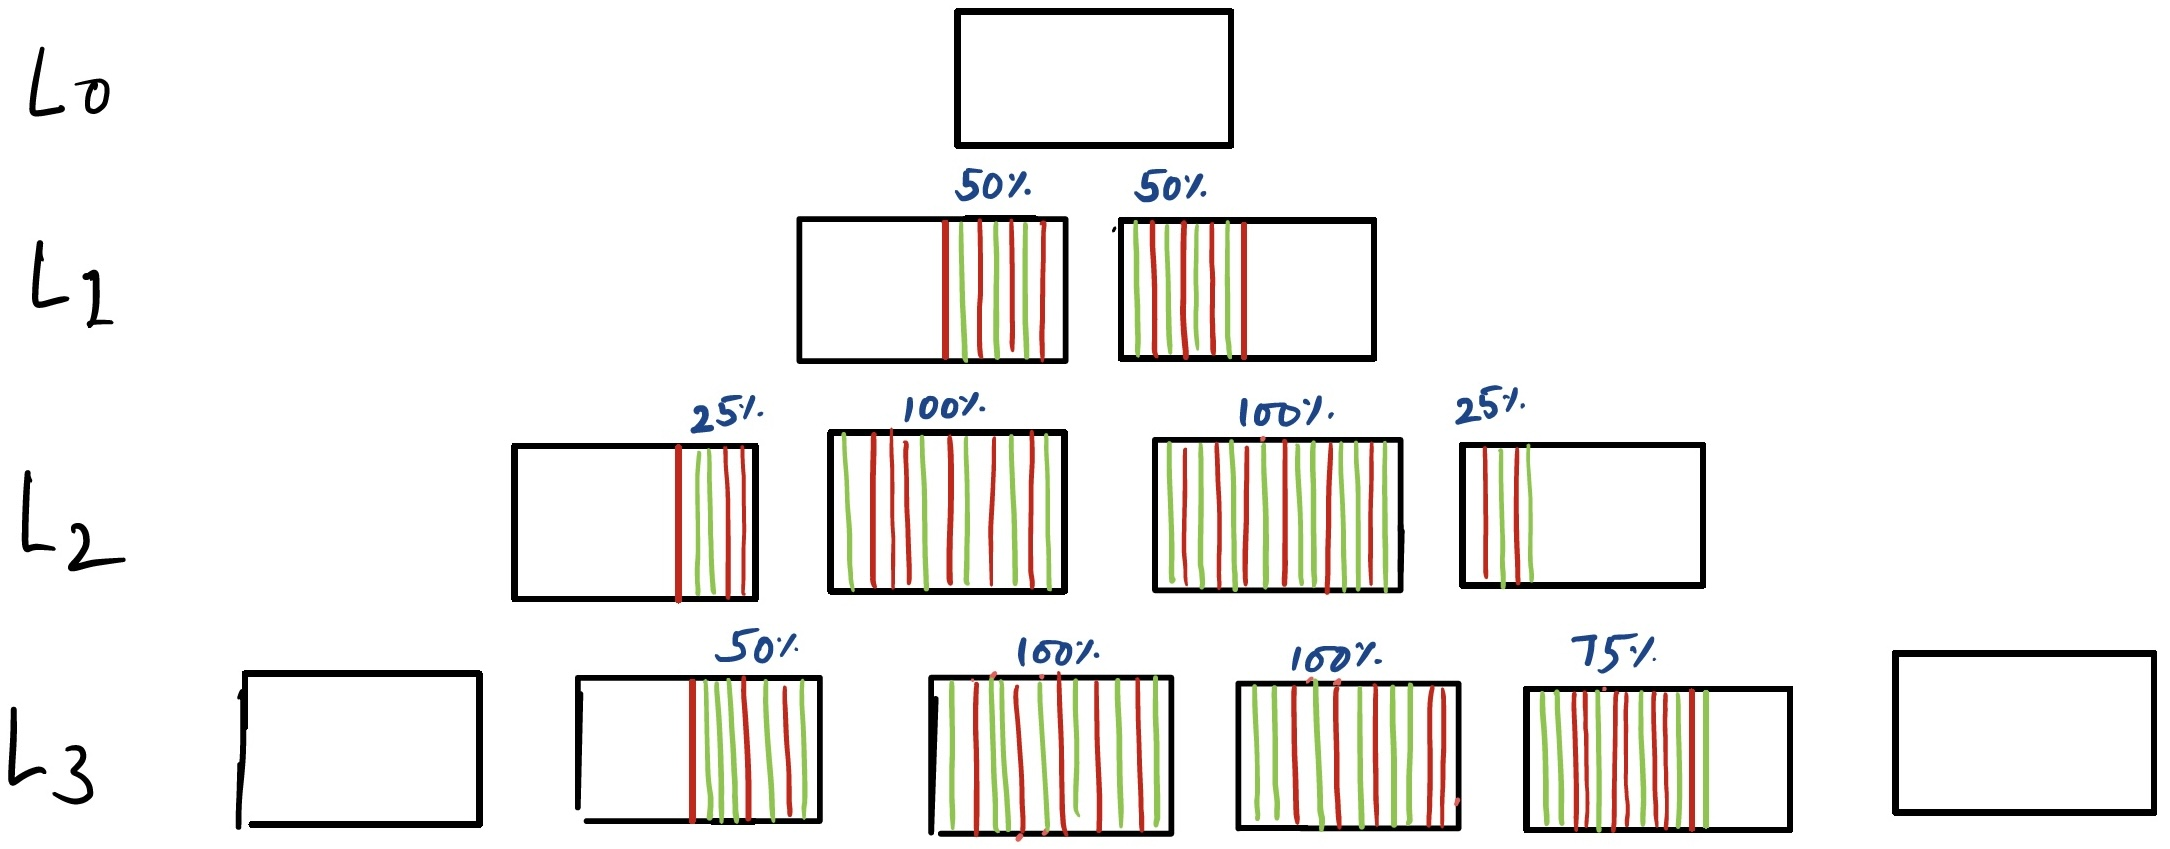
\includegraphics[scale=0.2]{Figures/first-state-lsm.jpg}
    \caption{Example to perfrom query-driven compaction}\label{fig:first-state-lsm}
\end{figure}


Let's take an example where we have an LSM with \textit{size ratio} 2 (T), number of pages 512 (P), 
number of entries per page 4 (B), and entry size 1024 B (E). Now, assume we have 4 levels in current LSM state 
(see Fig-\ref{fig:first-state-lsm}).

\begin{itemize}
    \item Page size $\colon B * E \approx 4 KB$
    \item File size $\colon P * B * E \approx 2 MB$
    \item Total entries in file $\colon P * B \approx 2 K$
    \item $WC_{threshold} \colon 0.5$
    \item $UTL_{threshold} \colon 0.4\ \&\ LTU_{threshold} \colon 1$ 
\end{itemize}

All the levels upto L2 are full and L3 has 6 files. This means we have approx 4K entries in L1 (2 SSTs), 8K in 
L2 (4 SSTs) and 12K in L3 (6 SSTs) as shown in Fig-\ref{fig:first-state-lsm}.

\begin{table}
    \resizebox{\linewidth}{!}{%
    \begin{tabular}{|c|c|c|c|c|c|}
        \hline
        \textbf{Level} & \textbf{\# of $E_{useful}$} & \textbf{\# of $E_{unuseful}$} & \textbf{min key} & \textbf{max key} & \textbf{\# of Entries} \\
        \hline
        L-0 & \-- & \-- & \-- & \-- & \--\\
        \hline
        L-1 & 2K & 2K & $x_{1}$ & $y_{1}$ & 2K \\
        \hline
        L-2 & 5K & 3K & $x_{2}$ & $y_{2}$ & 5K \\
        \hline
        L-3 & 6.5K & 1.5K & $x_{3}$ & $y_{3}$ & 6.5K \\
        \hline
    \end{tabular}}
    \caption{Decision making data for example shown in Fig-\ref{fig:first-state-lsm}}
    \label{table:ex-decision-making-meta-data}
\end{table}

\begin{table}
    % \captionsetup{justification=centering,margin=2cm}
    \begin{tabular}{ |c|c|c|c| }
        \hline
        \textbf{Level} & \textbf{L-1} & \hspace*{4.1mm}\textbf{L-2}\hspace*{4.1mm} & \hspace*{4.1mm}\textbf{L-3}\hspace*{4.1mm} \\
        \hline
        \textbf{L-1} & [0.5, -] = T & [0.58, (-, 0.4)] = T & [0.67, (-, 0.4, 0.76)] = T \\
        \hline
        \textbf{L-2} & $\times$ & [0.62, -] = T & [0.71, (-, 0.76)] = T \\
        \hline
        \textbf{L-3} &  $\times$ &  $\times$ & [0.81, -] = T \\
        \hline
    \end{tabular}
    \caption{Decision matrix based on Table-\ref{table:ex-decision-making-meta-data} (Cell: $[R_{utu}, R_{ete}]$)}
    \label{table:ex-decision-matrix}
\end{table}

\begin{table*}
    \centering
    \begin{tabular}{ccc}

        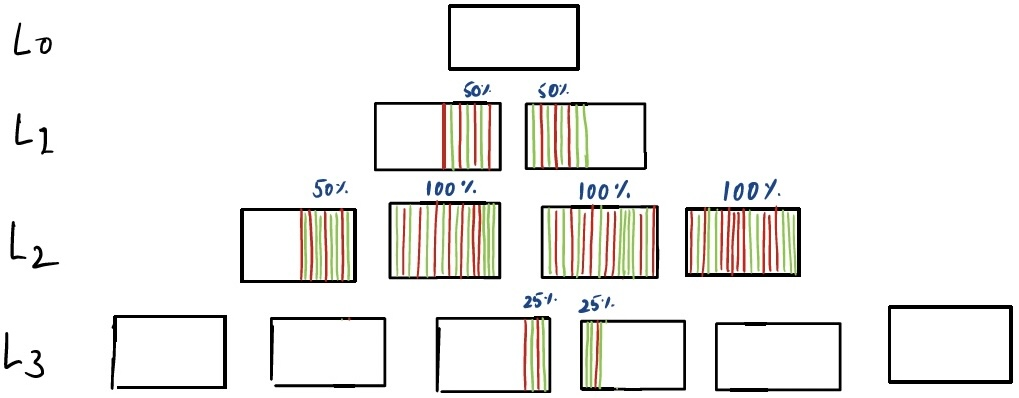
\includegraphics[scale=0.30]{Figures/fail-lsm-1.jpg} & 
        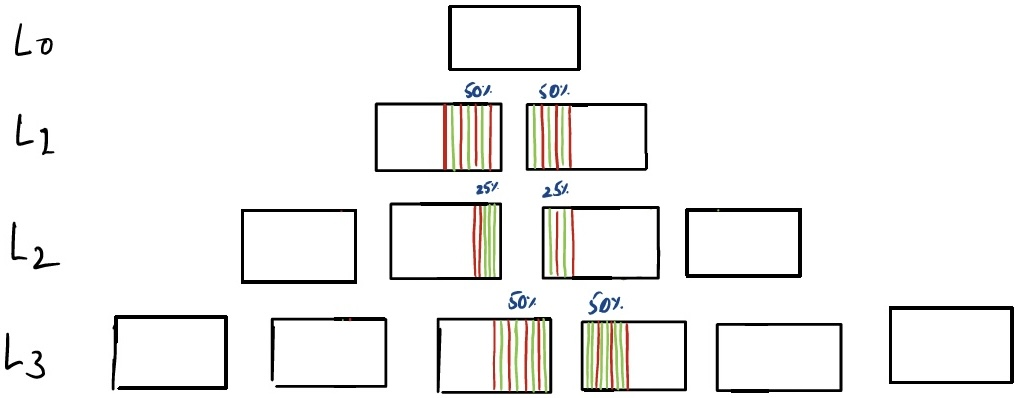
\includegraphics[scale=0.30]{Figures/fail-lsm-2.jpg} & 
        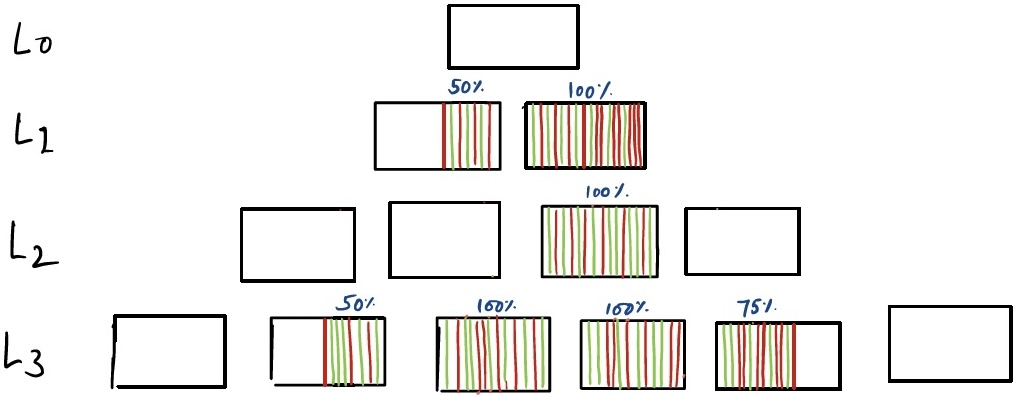
\includegraphics[scale=0.30]{Figures/fail-lsm-3.jpg}  \vspace{0.5em}\\

        \resizebox{0.3\textwidth}{!}{%
        \begin{tabular}{|c|c|c|c|c|c|}
            \hline
            \textbf{Level} & \textbf{\# of $E_{useful}$} & \textbf{\# of $E_{unuseful}$} & \textbf{min key} & \textbf{max key} & \textbf{\# of Entries} \\
            \hline
            L-0 & \-- & \-- & \-- & \-- & \--\\
            \hline
            L-1 & 2K & 2K & $x_{1}$ & $y_{1}$ & 2K \\
            \hline
            L-2 & 7K & 1K & $x_{2}$ & $y_{2}$ & 7K \\
            \hline
            L-3 & 0.5K & 2.5K & $x_{3}$ & $y_{3}$ & 0.5K \\
            \hline
        \end{tabular}}

        &

        \resizebox{0.3\textwidth}{!}{%
        \begin{tabular}{|c|c|c|c|c|c|}
            \hline
            \textbf{Level} & \textbf{\# of $E_{useful}$} & \textbf{\# of $E_{unuseful}$} & \textbf{min key} & \textbf{max key} & \textbf{\# of Entries} \\
            \hline
            L-0 & \-- & \-- & \-- & \-- & \--\\
            \hline
            L-1 & 2K & 2K & $x_{1}$ & $y_{1}$ & 2K \\
            \hline
            L-2 & 1K & 3K & $x_{2}$ & $y_{2}$ & 1K \\
            \hline
            L-3 & 2K & 2K & $x_{3}$ & $y_{3}$ & 2K \\
            \hline
        \end{tabular}}

        &

        \resizebox{0.3\textwidth}{!}{%
        \begin{tabular}{|c|c|c|c|c|c|}
            \hline
            \textbf{Level} & \textbf{\# of $E_{useful}$} & \textbf{\# of $E_{unuseful}$} & \textbf{min key} & \textbf{max key} & \textbf{\# of Entries} \\
            \hline
            L-0 & \-- & \-- & \-- & \-- & \--\\
            \hline
            L-1 & 3K & 1K & $x_{1}$ & $y_{1}$ & 3K \\
            \hline
            L-2 & 2K & 0K & $x_{2}$ & $y_{2}$ & 2K \\
            \hline
            L-3 & 6.5K & 1.5K & $x_{3}$ & $y_{3}$ & 6.5K \\
            \hline
        \end{tabular}} \vspace{0.5em}\\
    
        \resizebox{0.3\textwidth}{!}{%
        \begin{tabular}{ |c|c|c|c| }
            \hline
            \textbf{Level} & \textbf{L-1} & \hspace*{4.1mm}\textbf{L-2}\hspace*{4.1mm} & \hspace*{4.1mm}\textbf{L-3}\hspace*{4.1mm} \\
            \hline
            \textbf{L-1} & [0.5, -] = T & [0.75, (-, 0.28)] = F & [0.63, (-, 0.28, 14)] = F \\
            \hline
            \textbf{L-2} & $\times$ & [0.87, -] = T & [0.68, (-, 14)] = F \\
            \hline
            \textbf{L-3} &  $\times$ &  $\times$ & [0.2, -] = F \\
            \hline
        \end{tabular}}
        
        &

        \resizebox{0.3\textwidth}{!}{%
        \begin{tabular}{ |c|c|c|c| }
            \hline
            \textbf{Level} & \textbf{L-1} & \hspace*{4.1mm}\textbf{L-2}\hspace*{4.1mm} & \hspace*{4.1mm}\textbf{L-3}\hspace*{4.1mm} \\
            \hline
            \textbf{L-1} & [0.5, -] = T & [0.37, (-, 2)] = F & [0.41, (-, 2, 0.5)] = F \\
            \hline
            \textbf{L-2} & $\times$ & [0.25, -] = F & [0.37, (-, 0.5)] = F \\
            \hline
            \textbf{L-3} &  $\times$ &  $\times$ & [0.5, -] = T \\
            \hline
        \end{tabular}}

        &

        \resizebox{0.3\textwidth}{!}{%
        \begin{tabular}{ |c|c|c|c| }
            \hline
            \textbf{Level} & \textbf{L-1} & \hspace*{4.1mm}\textbf{L-2}\hspace*{4.1mm} & \hspace*{4.1mm}\textbf{L-3}\hspace*{4.1mm} \\
            \hline
            \textbf{L-1} & [0.75, -] = T & [0.83, (-, 1.5)] = F & [0.82, (-, 1.5, 0.30)] = F \\
            \hline
            \textbf{L-2} & $\times$ & [1, -] = T & [0.85, (-, 0.30)] = F \\
            \hline
            \textbf{L-3} &  $\times$ &  $\times$ & [0.81, -] = T \\
            \hline
        \end{tabular}}
    \end{tabular}
    \caption{Examples for NOT performing query-driven compaction based on decision matrix}
    \label{table:ex-not-performing-compaction}
\end{table*}

Now, consider a range query (shaded portion in Fig-\ref{fig:first-state-lsm}) that will read entries from L1, L2, and L3.
The $E_{useful}$ and $E_{unuseful}$ would be as shown in Table-\ref{table:ex-decision-making-meta-data}. 
The \textit{min\_key} \& \textit{max\_key} are the minimum and maximum keys of the range query from each level. 
The decision matrix can be formed based on Table-\ref{table:ex-decision-making-meta-data} (as shown in 
Table-\ref{table:ex-decision-matrix}). For this example we assume that the range of keys from every level are uniformly
overlapping with the range of keys on the next level. The query-driven compaction will pick the first true entry from 
right top of the decision matrix checking every diagonal from left top to the right botton of the matrix. For the above 
example it would be $L_{13}$.







% \begin{figure}
%     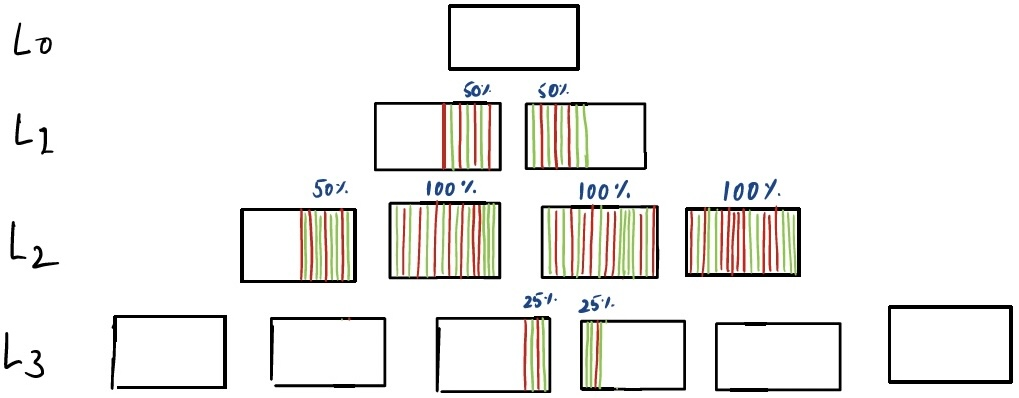
\includegraphics[scale=0.45]{Figures/fail-lsm-1.jpg}
%     \caption{Ex-1 don't perform query-driven compaction}\label{fig:fail-lsm-1}
% \end{figure}


% \begin{table}
%     \resizebox{\linewidth}{!}{%
%     \begin{tabular}{|c|c|c|c|c|c|}
%         \hline
%         \textbf{Level} & \textbf{\# of $E_{useful}$} & \textbf{\# of $E_{unuseful}$} & \textbf{min key} & \textbf{max key} & \textbf{\# of Entries} \\
%         \hline
%         L-0 & \-- & \-- & \-- & \-- & \--\\
%         \hline
%         L-1 & 2K & 2K & $x_{1}$ & $y_{1}$ & 2K \\
%         \hline
%         L-2 & 7K & 1K & $x_{2}$ & $y_{2}$ & 7K \\
%         \hline
%         L-3 & 0.5K & 2.5K & $x_{3}$ & $y_{3}$ & 0.5K \\
%         \hline
%     \end{tabular}}
%     \caption{Decision making data for example shown in Fig-\ref{fig:fail-lsm-1}}
%     \label{table:ex-not-perform-rqdc-1}
% \end{table}

% \begin{table}
%     \begin{tabular}{ |c|c|c|c| }
%         \hline
%         \textbf{Level} & \textbf{L-1} & \hspace*{4.1mm}\textbf{L-2}\hspace*{4.1mm} & \hspace*{4.1mm}\textbf{L-3}\hspace*{4.1mm} \\
%         \hline
%         \textbf{L-1} & [0.5, -] = T & [0.75, (-, 0.28)] = F & [0.63, (-, 0.28, 14)] = F \\
%         \hline
%         \textbf{L-2} & $\times$ & [0.87, -] = T & [0.68, (-, 14)] = F \\
%         \hline
%         \textbf{L-3} &  $\times$ &  $\times$ & [0.2, -] = F \\
%         \hline
%     \end{tabular}
%     \caption{Decision matrix based on Table-\ref{table:ex-not-perform-rqdc-1} (Cell: $[R_{utu}, R_{ete}]$)}
%     \label{table:ex-matrix-not-perform-rqdc-1}
% \end{table}

% \begin{figure}
%     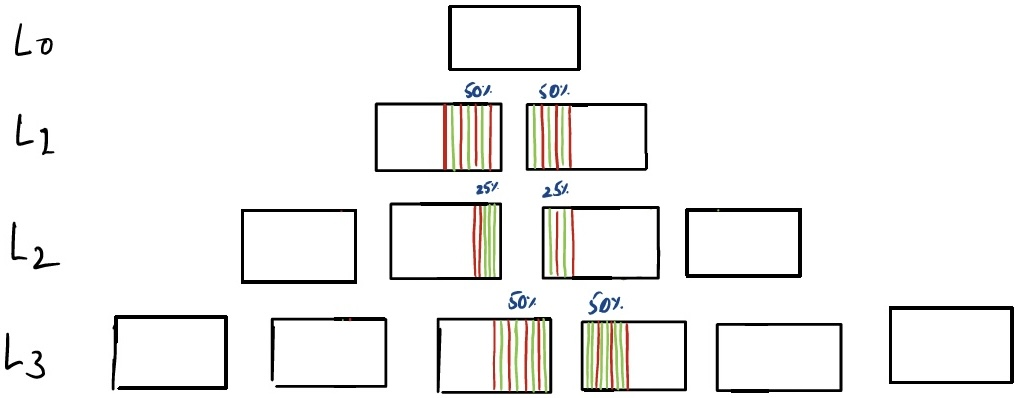
\includegraphics[scale=0.45]{Figures/fail-lsm-2.jpg}
%     \caption{Ex-2 don't perform query-driven compaction}\label{fig:fail-lsm-2}
% \end{figure}

% \begin{table}
%     \resizebox{\linewidth}{!}{%
%     \begin{tabular}{|c|c|c|c|c|c|}
%         \hline
%         \textbf{Level} & \textbf{\# of $E_{useful}$} & \textbf{\# of $E_{unuseful}$} & \textbf{min key} & \textbf{max key} & \textbf{\# of Entries} \\
%         \hline
%         L-0 & \-- & \-- & \-- & \-- & \--\\
%         \hline
%         L-1 & 2K & 2K & $x_{1}$ & $y_{1}$ & 2K \\
%         \hline
%         L-2 & 1K & 3K & $x_{2}$ & $y_{2}$ & 1K \\
%         \hline
%         L-3 & 2K & 2K & $x_{3}$ & $y_{3}$ & 2K \\
%         \hline
%     \end{tabular}}
%     \caption{Decision making data for example shown in Fig-\ref{fig:fail-lsm-2}}
%     \label{table:ex-not-perform-rqdc-2}
% \end{table}

% \begin{table}
%     \begin{tabular}{ |c|c|c|c| }
%         \hline
%         \textbf{Level} & \textbf{L-1} & \hspace*{4.1mm}\textbf{L-2}\hspace*{4.1mm} & \hspace*{4.1mm}\textbf{L-3}\hspace*{4.1mm} \\
%         \hline
%         \textbf{L-1} & [0.5, -] = T & [0.37, (-, 2)] = F & [0.41, (-, 2, 0.5)] = F \\
%         \hline
%         \textbf{L-2} & $\times$ & [0.25, -] = F & [0.37, (-, 0.5)] = F \\
%         \hline
%         \textbf{L-3} &  $\times$ &  $\times$ & [0.5, -] = T \\
%         \hline
%     \end{tabular}
%     \caption{Decision matrix based on Table-\ref{table:ex-not-perform-rqdc-2} (Cell: $[R_{utu}, R_{ete}]$)}
%     \label{table:ex-matrix-not-perform-rqdc-2}
% \end{table}

% \begin{figure}
%     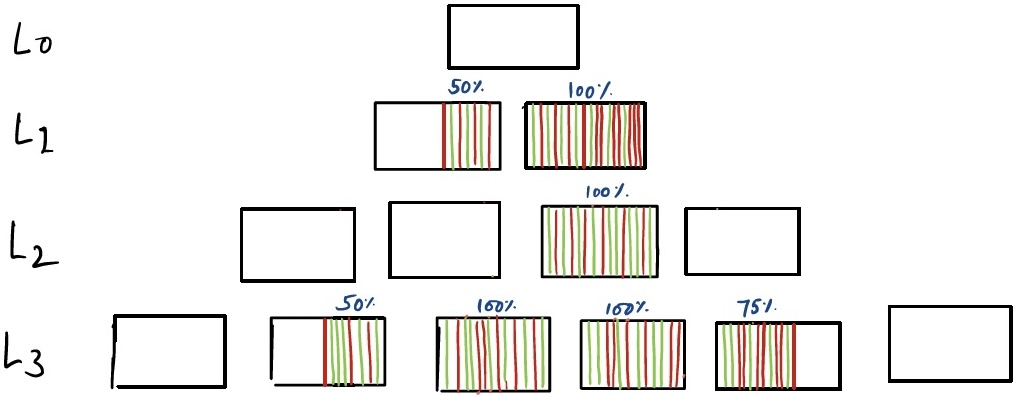
\includegraphics[scale=0.45]{Figures/fail-lsm-3.jpg}
%     \caption{Ex-3 don't perform query-driven compaction}\label{fig:fail-lsm-3}
% \end{figure}

% \begin{table}
%     \resizebox{\linewidth}{!}{%
%     \begin{tabular}{|c|c|c|c|c|c|}
%         \hline
%         \textbf{Level} & \textbf{\# of $E_{useful}$} & \textbf{\# of $E_{unuseful}$} & \textbf{min key} & \textbf{max key} & \textbf{\# of Entries} \\
%         \hline
%         L-0 & \-- & \-- & \-- & \-- & \--\\
%         \hline
%         L-1 & 3K & 1K & $x_{1}$ & $y_{1}$ & 3K \\
%         \hline
%         L-2 & 2K & 0K & $x_{2}$ & $y_{2}$ & 2K \\
%         \hline
%         L-3 & 6.5K & 1.5K & $x_{3}$ & $y_{3}$ & 6.5K \\
%         \hline
%     \end{tabular}}
%     \caption{Decision making data for example shown in Fig-\ref{fig:fail-lsm-3}}
%     \label{table:ex-not-perform-rqdc-3}
% \end{table}

% \begin{table}
%     \begin{tabular}{ |c|c|c|c| }
%         \hline
%         \textbf{Level} & \textbf{L-1} & \hspace*{4.1mm}\textbf{L-2}\hspace*{4.1mm} & \hspace*{4.1mm}\textbf{L-3}\hspace*{4.1mm} \\
%         \hline
%         \textbf{L-1} & [0.75, -] = T & [0.83, (-, 1.5)] = F & [0.82, (-, 1.5, 0.30)] = F \\
%         \hline
%         \textbf{L-2} & $\times$ & [1, -] = T & [0.85, (-, 0.30)] = F \\
%         \hline
%         \textbf{L-3} &  $\times$ &  $\times$ & [0.81, -] = T \\
%         \hline
%     \end{tabular}
%     \caption{Decision matrix based on Table-\ref{table:ex-not-perform-rqdc-3} (Cell: $[R_{utu}, R_{ete}]$)}
%     \label{table:ex-matrix-not-perform-rqdc-3}
% \end{table}

\begin{figure}
    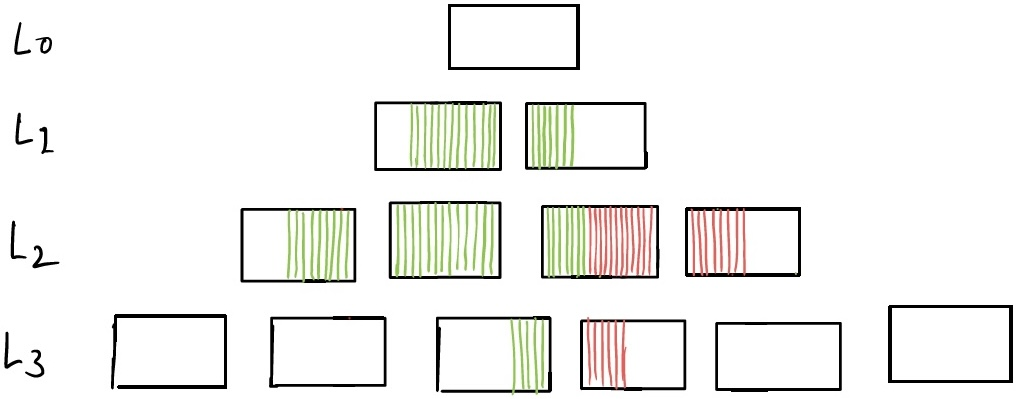
\includegraphics[scale=0.45]{Figures/extended-solution.jpg}
    \caption{Extended Solution}\label{fig:extended-solution}
\end{figure}


















% \begin{figure}
%     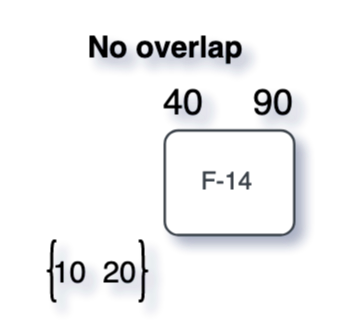
\includegraphics[scale=0.10]{Figures/No Overlap.png}
%     \caption{No Overlap between range-query and file}\label{fig:no_overlap}
% \end{figure}

% \begin{figure}
%     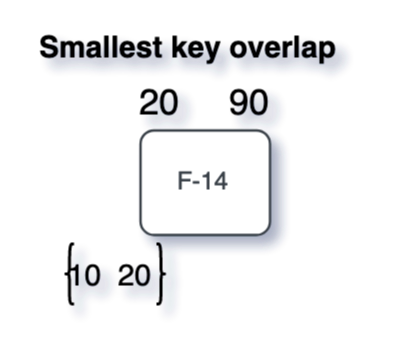
\includegraphics[scale=0.10]{Figures/Smallest Key Overlap.png}
%     \caption{Smallest (single) key overalp with range-query}\label{fig:smallest_key_overlap}
% \end{figure}

% \begin{figure}
%     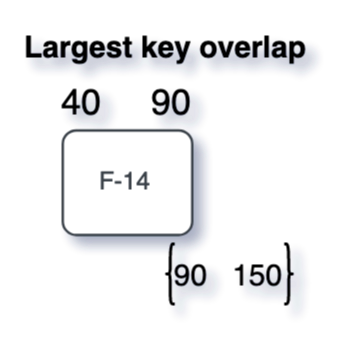
\includegraphics[scale=0.10]{Figures/Largest Key Overlap.png}
%     \caption{Largest (single) key overlap with range-query}\label{fig:largest_key_overlap}
% \end{figure}

% \begin{figure}
%     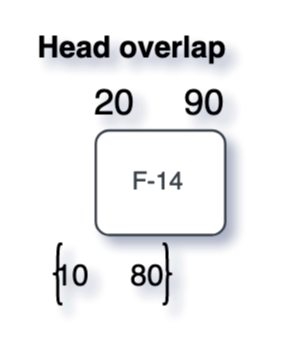
\includegraphics[scale=0.10]{Figures/Head Overlap.png}
%     \caption{Head (more than one key) overlap with range-query}\label{fig:head_overlap}
% \end{figure}

% \begin{figure}
%     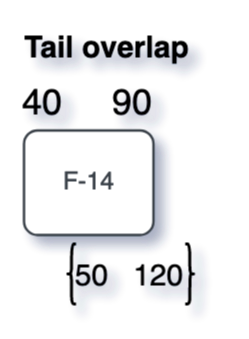
\includegraphics[scale=0.10]{Figures/Tail Overlap.png}
%     \caption{Tail (more than one key) overlap with range-query}\label{fig:tail_overlap}
% \end{figure}

% \begin{figure}
%     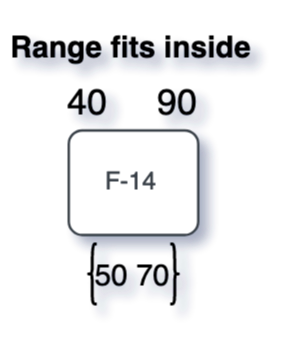
\includegraphics[scale=0.10]{Figures/Range Fits Overlap.png}
%     \caption{Range query overlap by file}\label{fig:range_fits_overlap}
% \end{figure}

% \begin{figure}
%     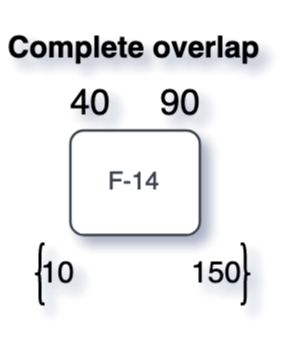
\includegraphics[scale=0.10]{Figures/Complete Overlap.png}
%     \caption{Complete file overlap}\label{fig:complete_overlap}
% \end{figure}



% \begin{table}
%     \captionsetup{justification=centering,margin=2cm}
%     \begin{tabular}{ |c|c|c|c| }
%         \hline
%         \textbf{Level} & \textbf{L-1} & \textbf{L-2} & \textbf{L-3} \\
%         \hline
%         \textbf{L-1} & $0.5$ & $0.5$ & $0.5$ \\
%         \hline
%         \textbf{L-2} & $\times$ & $0.625$ & $0.59$ \\
%         \hline
%         \textbf{L-3} &  $\times$ &  $\times$ & $0.812$ \\
%         \hline
%     \end{tabular}
%     \caption{Decision Matrix (assuming that each level is completely overlapping with next level range data)}
%     \label{table:ex-decision-matrix}
% \end{table}

% \section{Results}
% \label{sec:results}
% \input{5-analytical_results}

\section{Evaluation}
\label{sec:experimental_results}
In this section, we address two key problems outlined in the problem statement (Section 1.2):

\Paragraph{Redundant Work} One significant challenge arises when overlapping or identical range queries are executed in 
the database. The conventional approach performs the same amount of work for each query, involving a sort-merge 
operation across multiple levels to filter out invalid keys. However, a query-driven compaction strategy involves 
storing the result of the sort-merge operation from the initial range query at a higher level. By eliminating invalid 
keys at an earlier stage, subsequent overlapping range queries encounter reduced complexity. This leads to a more 
efficient execution, as later queries need to read fewer files, traverse fewer levels, and consequently encounter fewer 
invalid keys.

\Paragraph{Increased Write Amplification} The conventional method initiates compactions that retain invalid keys within 
the resulting SST files until they reach the last level, thereby causing a rise in write amplification. The query-driven
compaction strategy helps in eliminating invalid keys throughout the compaction process, resulting in a reduction of 
write amplification and a consequential enhancement in overall system efficiency.

The introduction of aggressive compactions during range queries may create gaps between levels and alter the tree shape. 
Paradoxically, this deformation proves advantageous for future ingestions, acting as a preventive measure against 
triggering cascading compactions. 

To substantiate these hypothesis, we conducted a series of experiments on an emulator, 
implementing the query-driven compaction approach. The results validated our expectations, demonstrating that queries 
following a query-driven compaction exhibited significantly improved speed. This optimization not only accelerates query 
execution but also enhances the overall efficiency of the ingestion process. To provide a more concrete understanding, 
we implemented the query-driven compaction approach on RocksDB and conducted a series of experiments to validate its 
performance in a real-world setting. The details of which are outlined below.

\subsection{Experimental Settings}
We ran our experiments on baremetal cloud instances provided by Chameleon. We used `compute skylake' machines to run all 
our experiements.

\begin{itemize}
    \item CPU(s)\:: 48 Cores
    \item RAM\:: 187 GiB
    \item RocksDB version\:: 8.5.0
\end{itemize}

\subsection{Experimental Results}
First set of experiements that we ran were based on our first approach, where each range query has to 
perform query-driven compaction without thinking about the number of entries overlapping between levels. The workload that
we used is as follows.
\begin{enumerate}[leftmargin=*,labelindent=0mm, itemsep=0.2\baselineskip]
    \item Number of Inserts \-- 500000
    \item Number of Updates \-- 250000, 500000, 750000
    \item Number of Range Queries \-- 100 
    \item Selectivity for Range Queries \-- 0.2, 0.4, 0.8
\end{enumerate}

\begin{figure}
    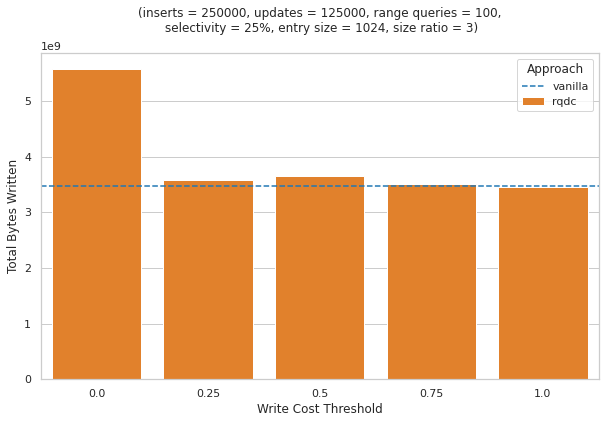
\includegraphics[scale=0.33]{Figures/utl_ltu_approach.png}
    \caption{Total write amplification in vanilla vs RQDC}\label{fig:utl_ltu_approach}
\end{figure}

The results show that the number of compactions triggered during the execution of the entire workload was significantly 
lower in the query-driven compaction than the vanilla approach (shown in Figure~\ref{fig:compaction_times}). This is 
expected since the query-driven approach performed these compactions during the range query executions. Additionally, 
the bytes written during background compactions are comparatively much less in our approach than in the vanilla approach
(shown in Figure~\ref{fig:compaction_write_bytes}) for the same reason. The Figure~\ref{fig:range_query_flush_write_bytes} 
shows the sum of bytes written during the ingestion of new keys and the bytes written during the query-driven compaction, 
which is almost 10x higher than the vanilla approach. The positive aspect is that this factor can be tuned by pre-computing 
the overlapping entries in the lower levels before performing the range query. If the lower levels have fewer entries 
that overlap with the higher level, then we can perform the vanilla fashion range query. However, if the overlap is more, 
then we can opt for query-driven compaction. These first set of experiments gave us a clear indication that we cannot 
use the query-driven approach for each range query blindly.

% \begin{figure*}
%     \begin{subfigure}{0.33\textwidth}
%         \centering
%         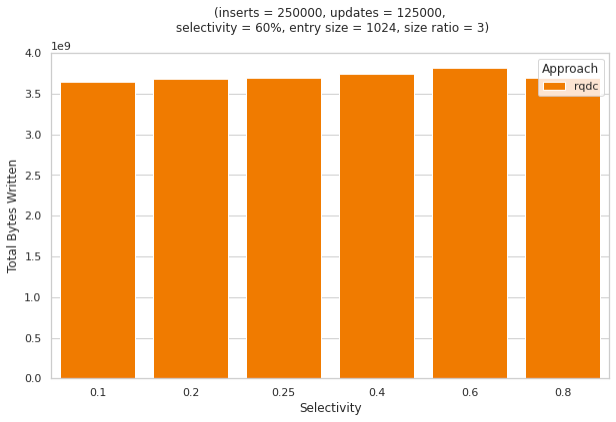
\includegraphics[width=\linewidth]{Figures/utl_ltu_with_varing_selectivity.png}
%         \caption{Total write amplification}\label{fig:utl_ltu_varing_selectivity}
%     \end{subfigure}%
%     \begin{subfigure}{0.33\textwidth}
%         \centering
%         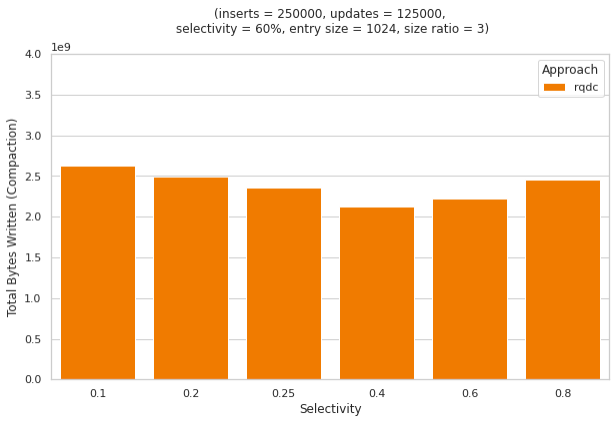
\includegraphics[width=\linewidth]{Figures/utl_ltu_varing_selectivity_compactions.png}
%         \caption{Compactions writes}\label{fig:utl_ltu_compaction_writes}
%     \end{subfigure}%
%     \begin{subfigure}{0.33\textwidth}
%         \centering
%         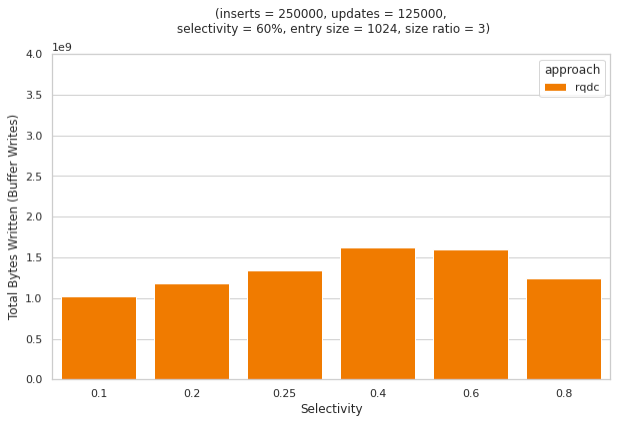
\includegraphics[width=\linewidth]{Figures/utl_ltu_varing_selectivity_flush.png}
%         \caption{Buffer writes}\label{fig:utl_ltu_buffer_writes}
%     \end{subfigure}
% \end{figure*}

\begin{figure}
    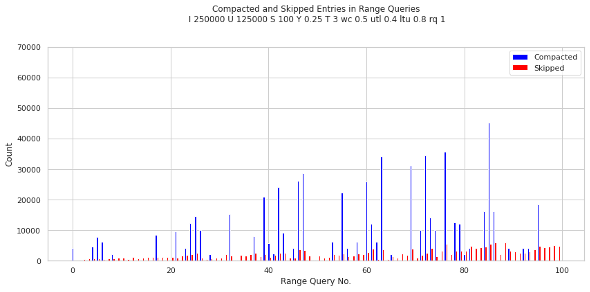
\includegraphics[scale=0.75]{Figures/compacted_vs_skipped.png}
    \caption{Compacted vs skipped keys during compaction}\label{fig:compacted_vs_skipped}
\end{figure}

We ran our second set of experiments using more informative compaction approach that we dicussed in section 4.3. The 
observations are as follows: the new approach has nearly the same write amplification as we have for vanilla but 
additionally provides a small benefit of reduced space amplification. The experiments were conducted for different $UTL$ and $LTU$ 
thresholds for a 25\% selectivity of range queries (shown in Figure~\ref{fig:utl_ltu_approach}). When the threshold is 
$0.0$, the compactions are performed blindly without thinking about the ovalapping entires.

% We also ran experiements with varying selectivites for the same number of range queries and found a slight bell curve for the write 
% amplications (shown in Figure~\ref{fig:utl_ltu_varing_selectivity},\ \ref{fig:utl_ltu_compaction_writes},\ \ref{fig:utl_ltu_buffer_writes}). 
% This was interesting, showing that for larger selectivities, the query-driven approach performs fewer compactions and 
% falls back to doing vanilla range queries because most of the data is already compacted due to previous range query compactions.

From these experiments we also observed that query-driven compaction compacts fairly large number of valid entries for the size ratio 3 (shown 
in Figure~\ref{fig:compacted_vs_skipped}). This might suggest that workloads benefiting from query-driven compaction 
should have more frequent updates, and the size ratio should be considerably larger. A smaller size ratio aids in 
promptly removing invalid keys as soon as updates are executed. This leads us to the next set of experimental design.

Our third set of experimental design was as follows: we ran the experiment in 11 epochs. The first epoch consisted only 
of inserts, set at 1 million to ensure our database was fully loaded. Subsequently, we ran 10 epochs with 25\% updates 
and 100 range queries of varying selectivities (10\% to 80\%). After each epoch, we recorded the total number of bytes 
written up to that point, the time taken by each range query in that epoch, and the total number of files and keys in 
our database. 

This set of experiments yielded promising results, as shown in Figure~\ref{fig:epoch_experiments}. The query-driven 
compaction approach wrote fewer bytes in every epoch after the 8th epoch. The level stats also showed that our approach 
had fewer files and fewer entries than vanilla. It removed a significant number of logically invalid entries during the 
compactions performed with range queries. This indicates that the query-driven approach outperformed the vanilla 
approach in terms of write and space amplification. This solves our second problem that we discussed above, namely 
``Increased Write Amplification''. 

\begin{figure}
    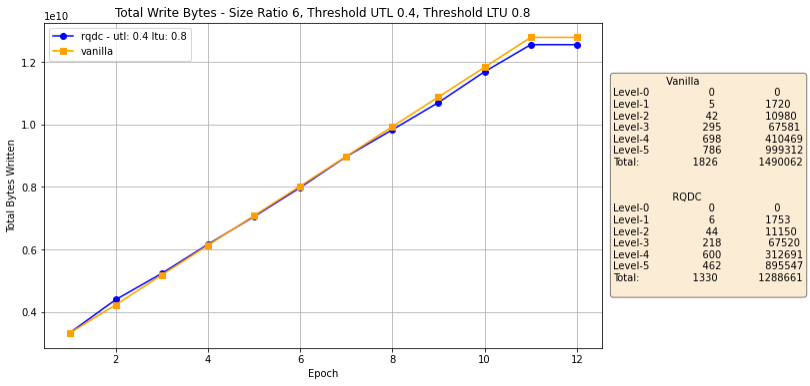
\includegraphics[scale=0.55]{Figures/epoch_experiments.png}
    \caption{Epoch experiments}\label{fig:epoch_experiments}
\end{figure}

\begin{figure}
    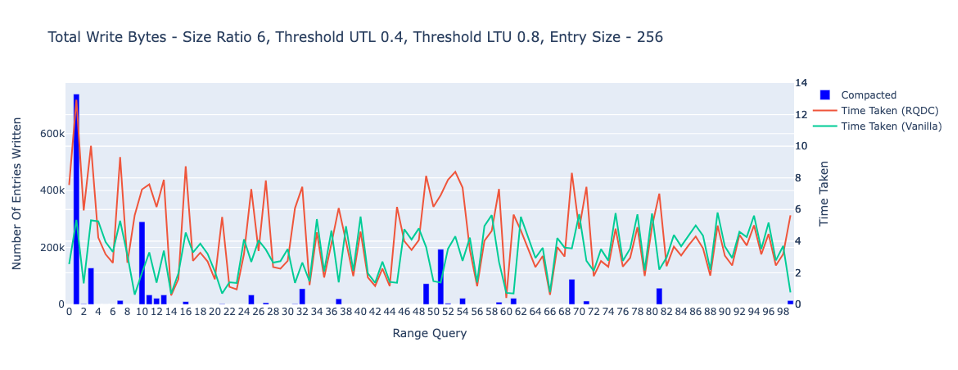
\includegraphics[scale=0.52]{Figures/first_epoch.png}
    \caption{First epoch updates and range queries}\label{fig:first_epoch}
\end{figure}

\begin{figure}
    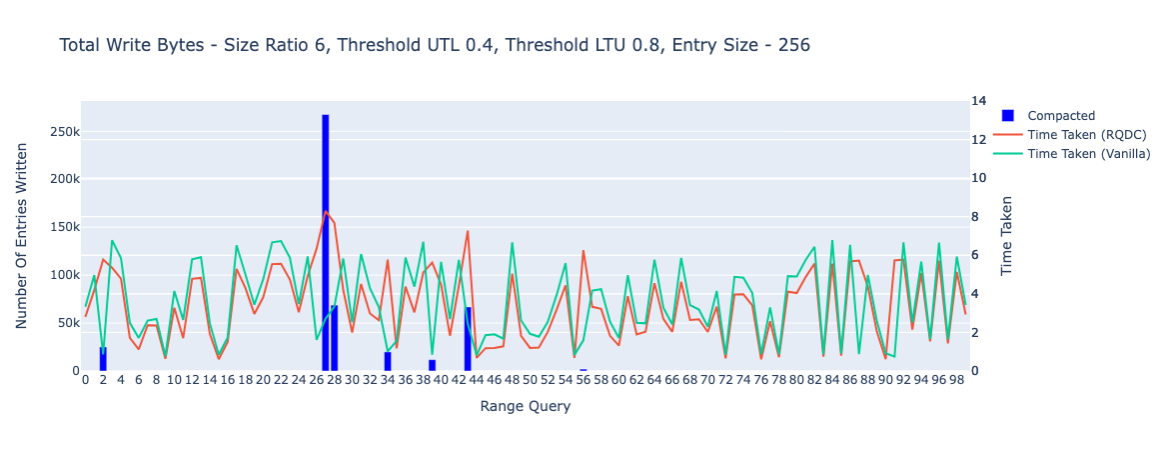
\includegraphics[scale=0.42]{Figures/last_epoch.png}
    \caption{Last epoch updates and range queries}\label{fig:last_epoch}
\end{figure}

We also observed the pattern of query-driven compaction through all of our epochs. The first epoch will have more 
opportunity to do the compactions since the lower levels are fully compact. The query driven compaction will take more 
time to perform the range query because of extra work performed with range query. The vanilla will take less time but 
stores more invalid keys to its levels. In the last few epochs the query-driven compaction will take less time to 
perform range queries because it will read few bytes than vanilla. We have shown the first and last epochs in 
Figure~\ref{fig:first_epoch},\ \ref{fig:last_epoch}.

Since we removed the invalid keys during the query-driven compaction, the subsequent range queries triggered after a 
successful execution of query-driven compaction will read fewer invalid keys (assuming the range is overlapping), 
leading to faster execution. This addresses our first problem of performing redundant work. Now, if the same range 
query is executed again, it may read only valid keys from the database.

% \begin{figure}
%     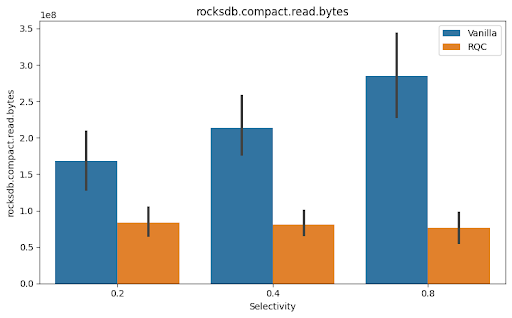
\includegraphics[scale=0.45]{Figures/Compaction Read Bytes.png}
%     \caption{Number of bytes read during compactions}\label{fig:compaction_read_bytes}
% \end{figure}

% Figure-\ref{fig:compaction_read_bytes} \& Figure-\ref{fig:compaction_write_bytes} shows the comparison between read and 
% writes bytes during the compactions that were triggered in vanilla and query-driven comapactions. We can see that the 
% bytes that were read and written during the vanilla are much higher than the newer approach

% \begin{figure}
%     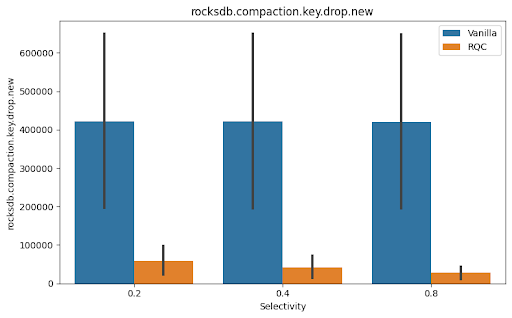
\includegraphics[scale=0.45]{Figures/Keys Drop In Compactions.png}
%     \caption{Number of keys dropped during compactions}\label{fig:keys_drop_in_compactions}
% \end{figure}

% Figure-\ref{fig:keys_drop_in_compactions} shows the number of keys that were dropped or re-written with newer values 
% while compaction.

% \begin{figure}
%     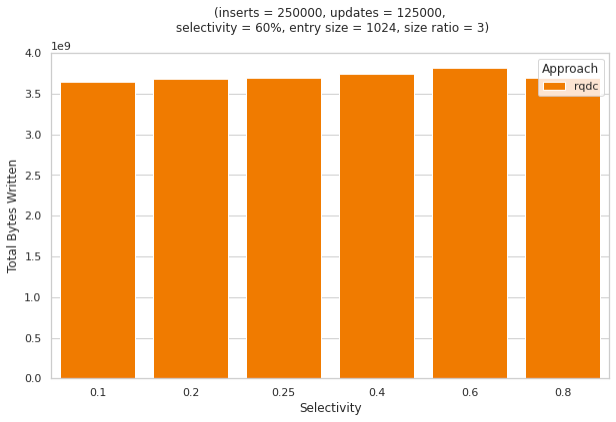
\includegraphics[scale=0.7]{Figures/utl_ltu_with_varing_selectivity.png}
%     \caption{Total write amplification in varing selectivity}\label{fig:utl_ltu_varing_selectivity}
% \end{figure}

% \begin{figure}
%     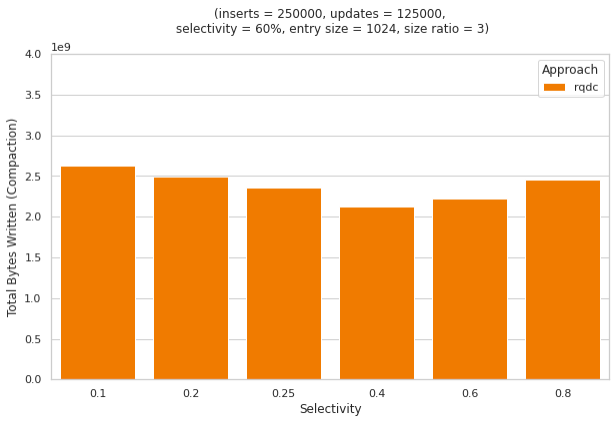
\includegraphics[scale=0.7]{Figures/utl_ltu_varing_selectivity_compactions.png}
%     \caption{Compactions writes in varing selectivity}\label{fig:utl_ltu_compaction_writes}
% \end{figure}

% \begin{figure}
%     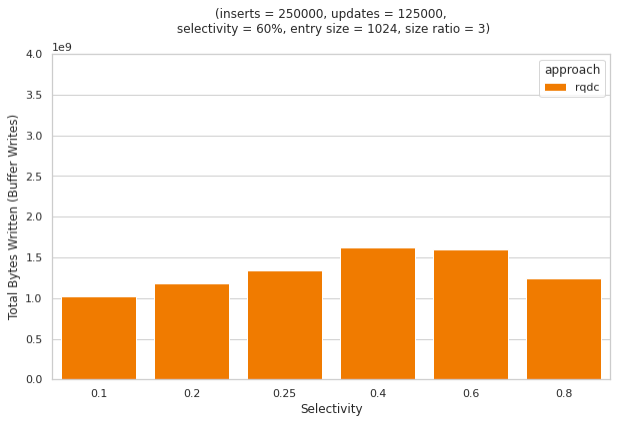
\includegraphics[scale=0.7]{Figures/utl_ltu_varing_selectivity_flush.png}
%     \caption{Buffer writes in varing selectivity}\label{fig:utl_ltu_buffer_writes}
% \end{figure}


\section{Related Work}
\label{sec:related_work}
\begin{figure}
    \centering
    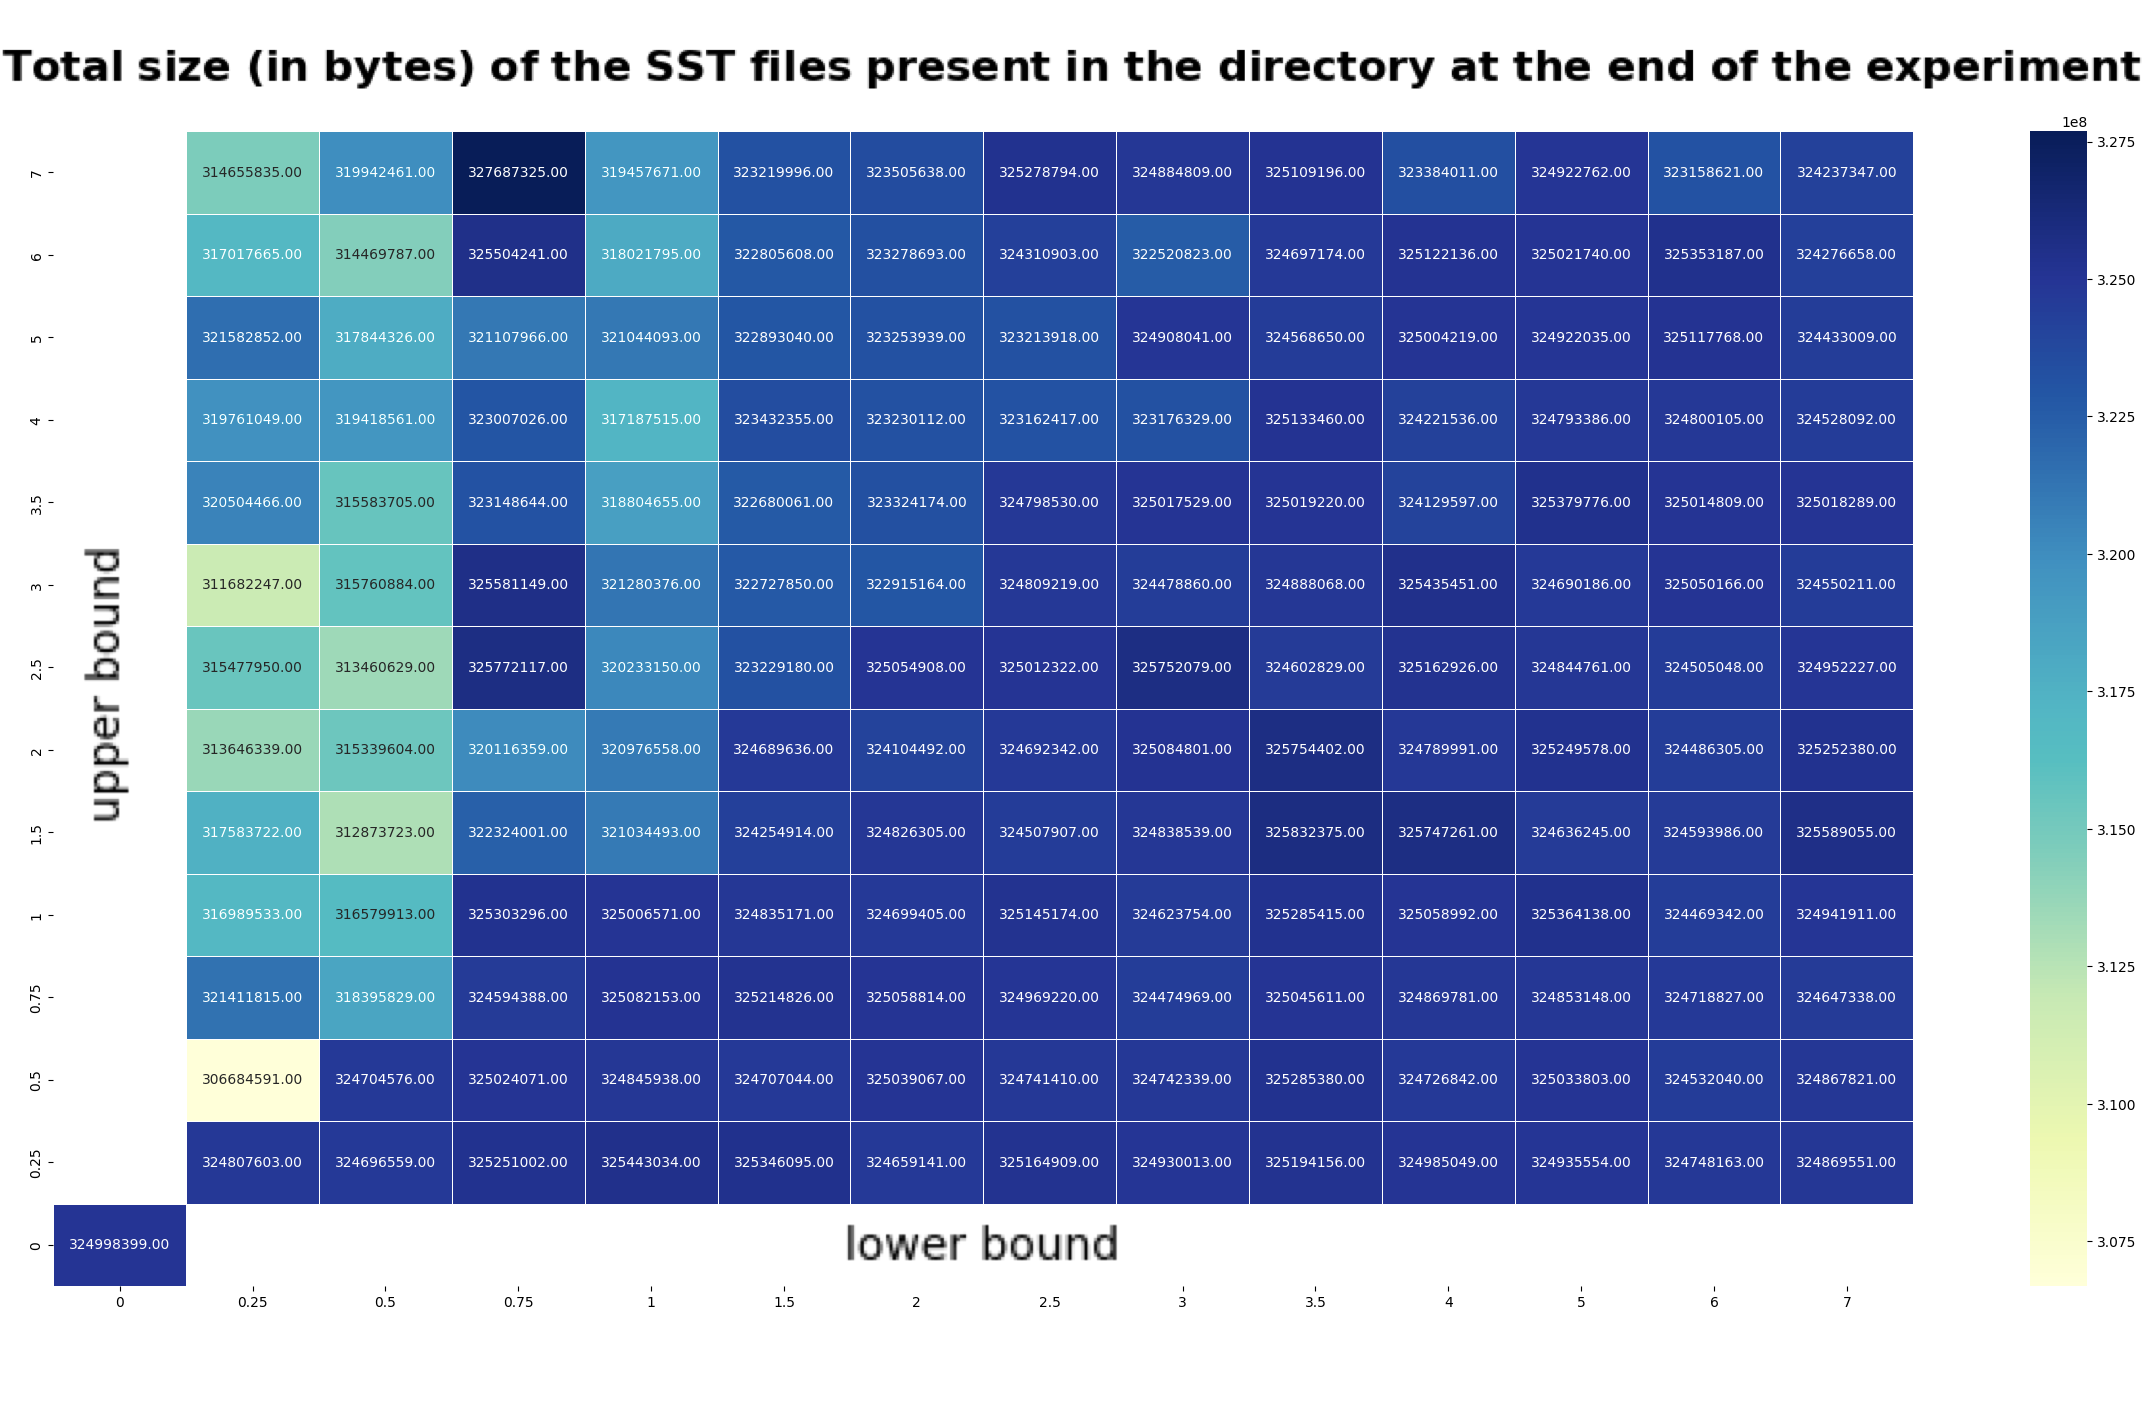
\includegraphics[width=\linewidth]{Figures/size-of-database.png}
    \caption{Figure shows how the size of database changes with different values of lower bound and upper bound.
    The horizontal axis shows the lower bound and vertical shows the upper bound. The left bottom corner shows the 
    Vanilla and rest all are for RQDC.}\label{fig:db_size_for_different_ub_lb}
\end{figure}

\begin{figure}
    \centering
    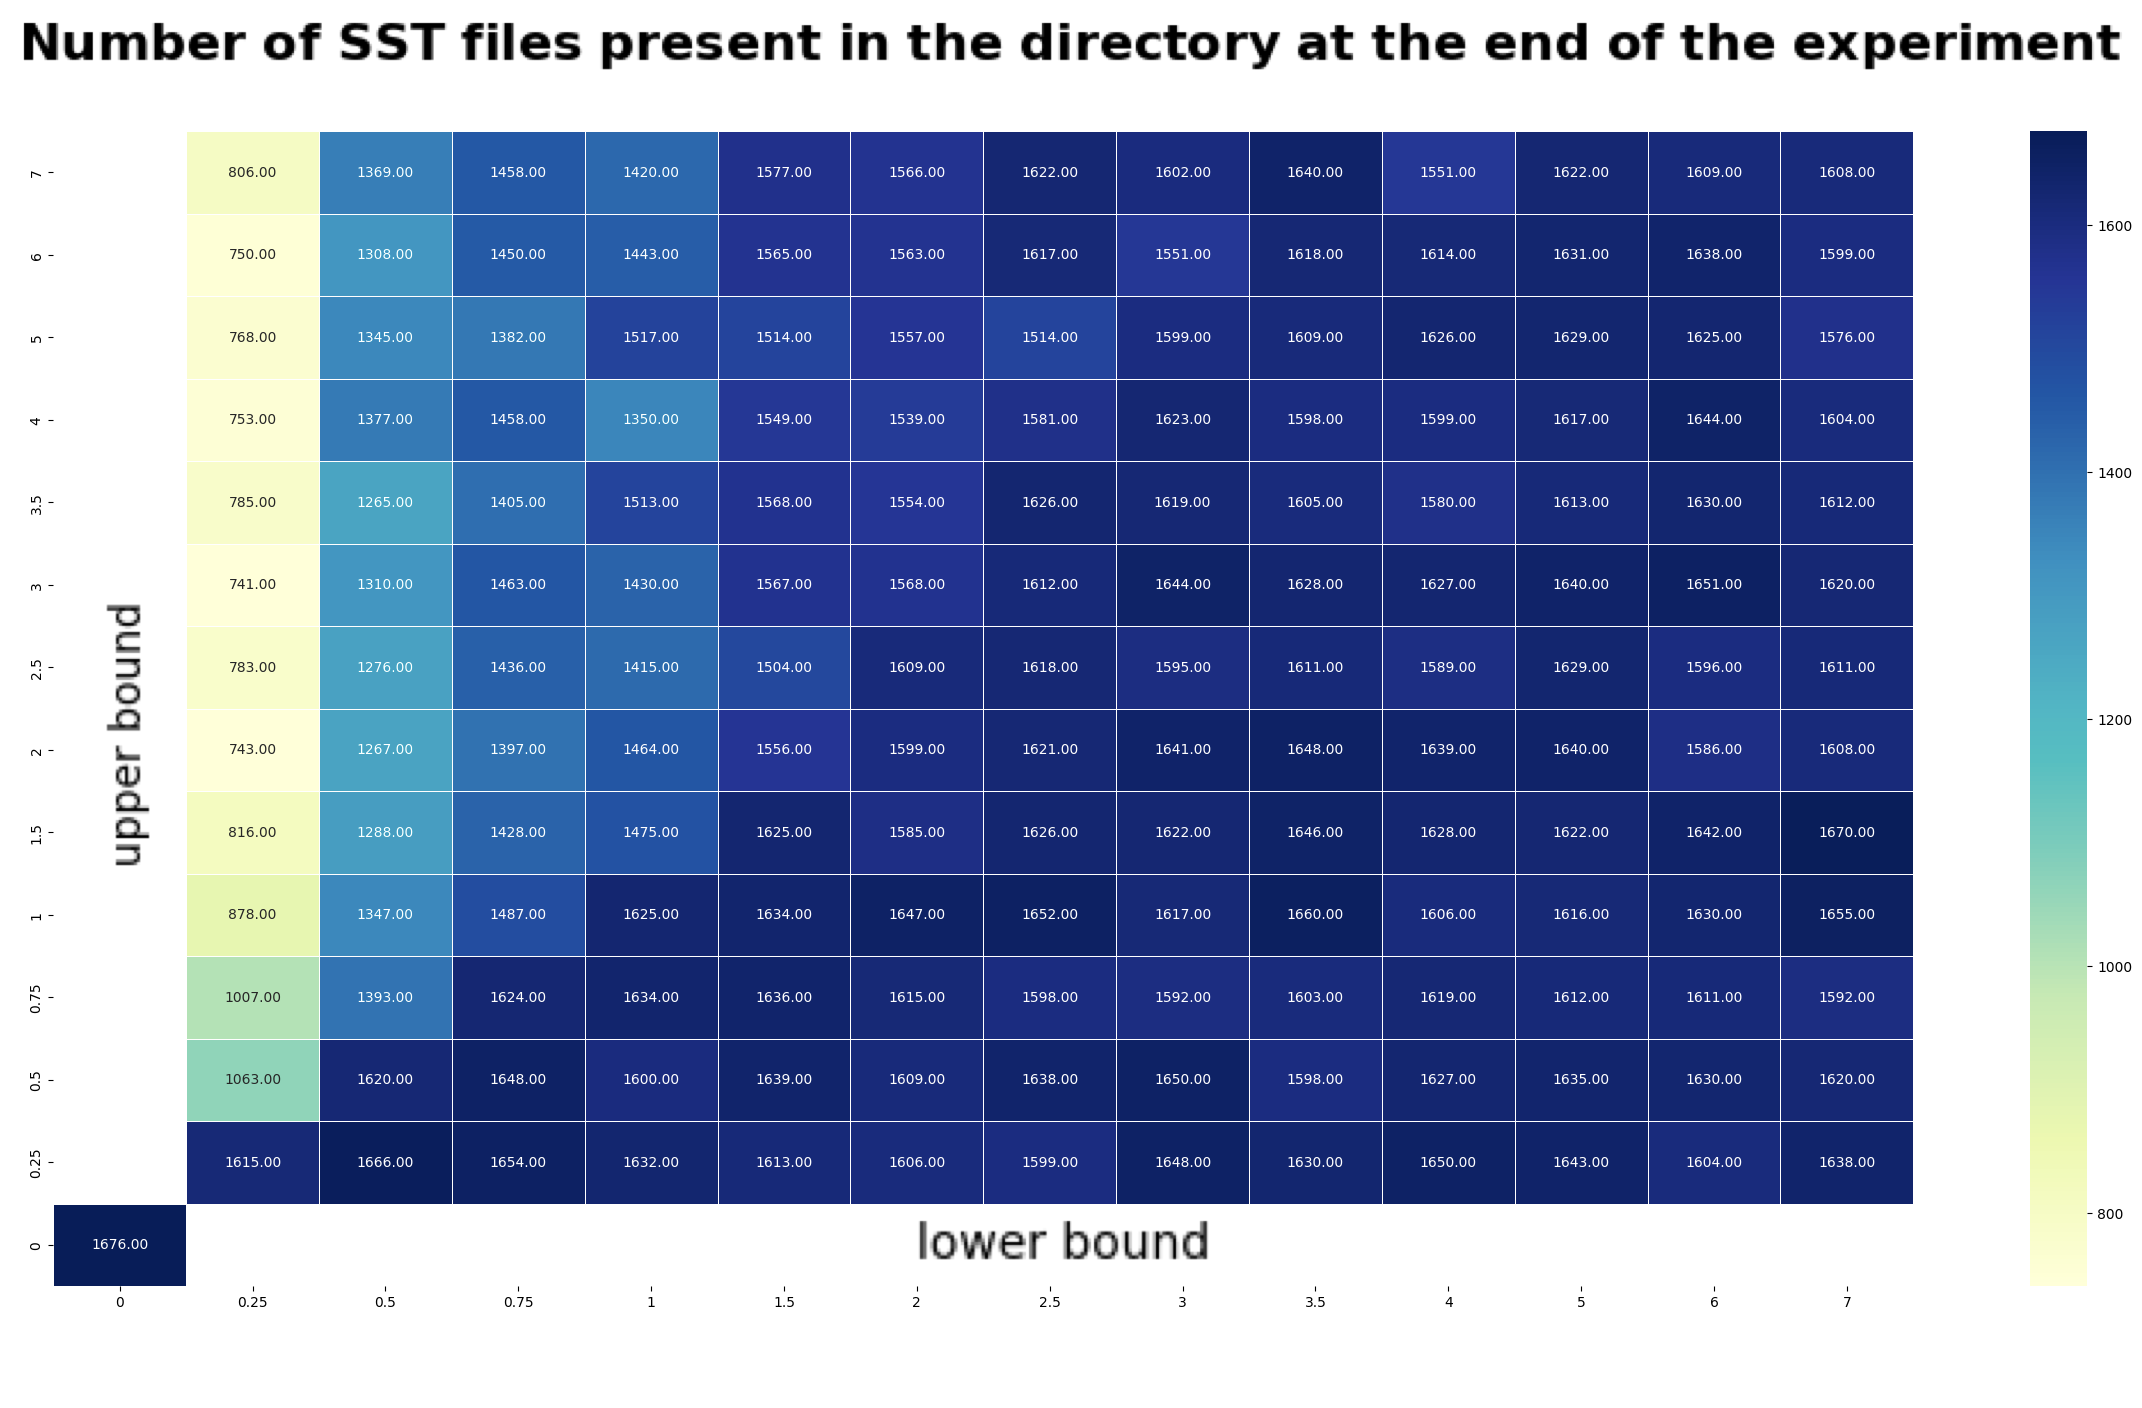
\includegraphics[width=\linewidth]{Figures/number-of-sst-files.png}
    \caption{Figure shows how the number of SST files changes with different values of lower bound and upper bound.
    The horizontal axis shows the lower bound and vertical shows the upper bound. The left bottom corner shows the 
    Vanilla and rest all are for RQDC.}\label{fig:number_of_sst_files_ub_lb}
\end{figure}

\begin{figure}
    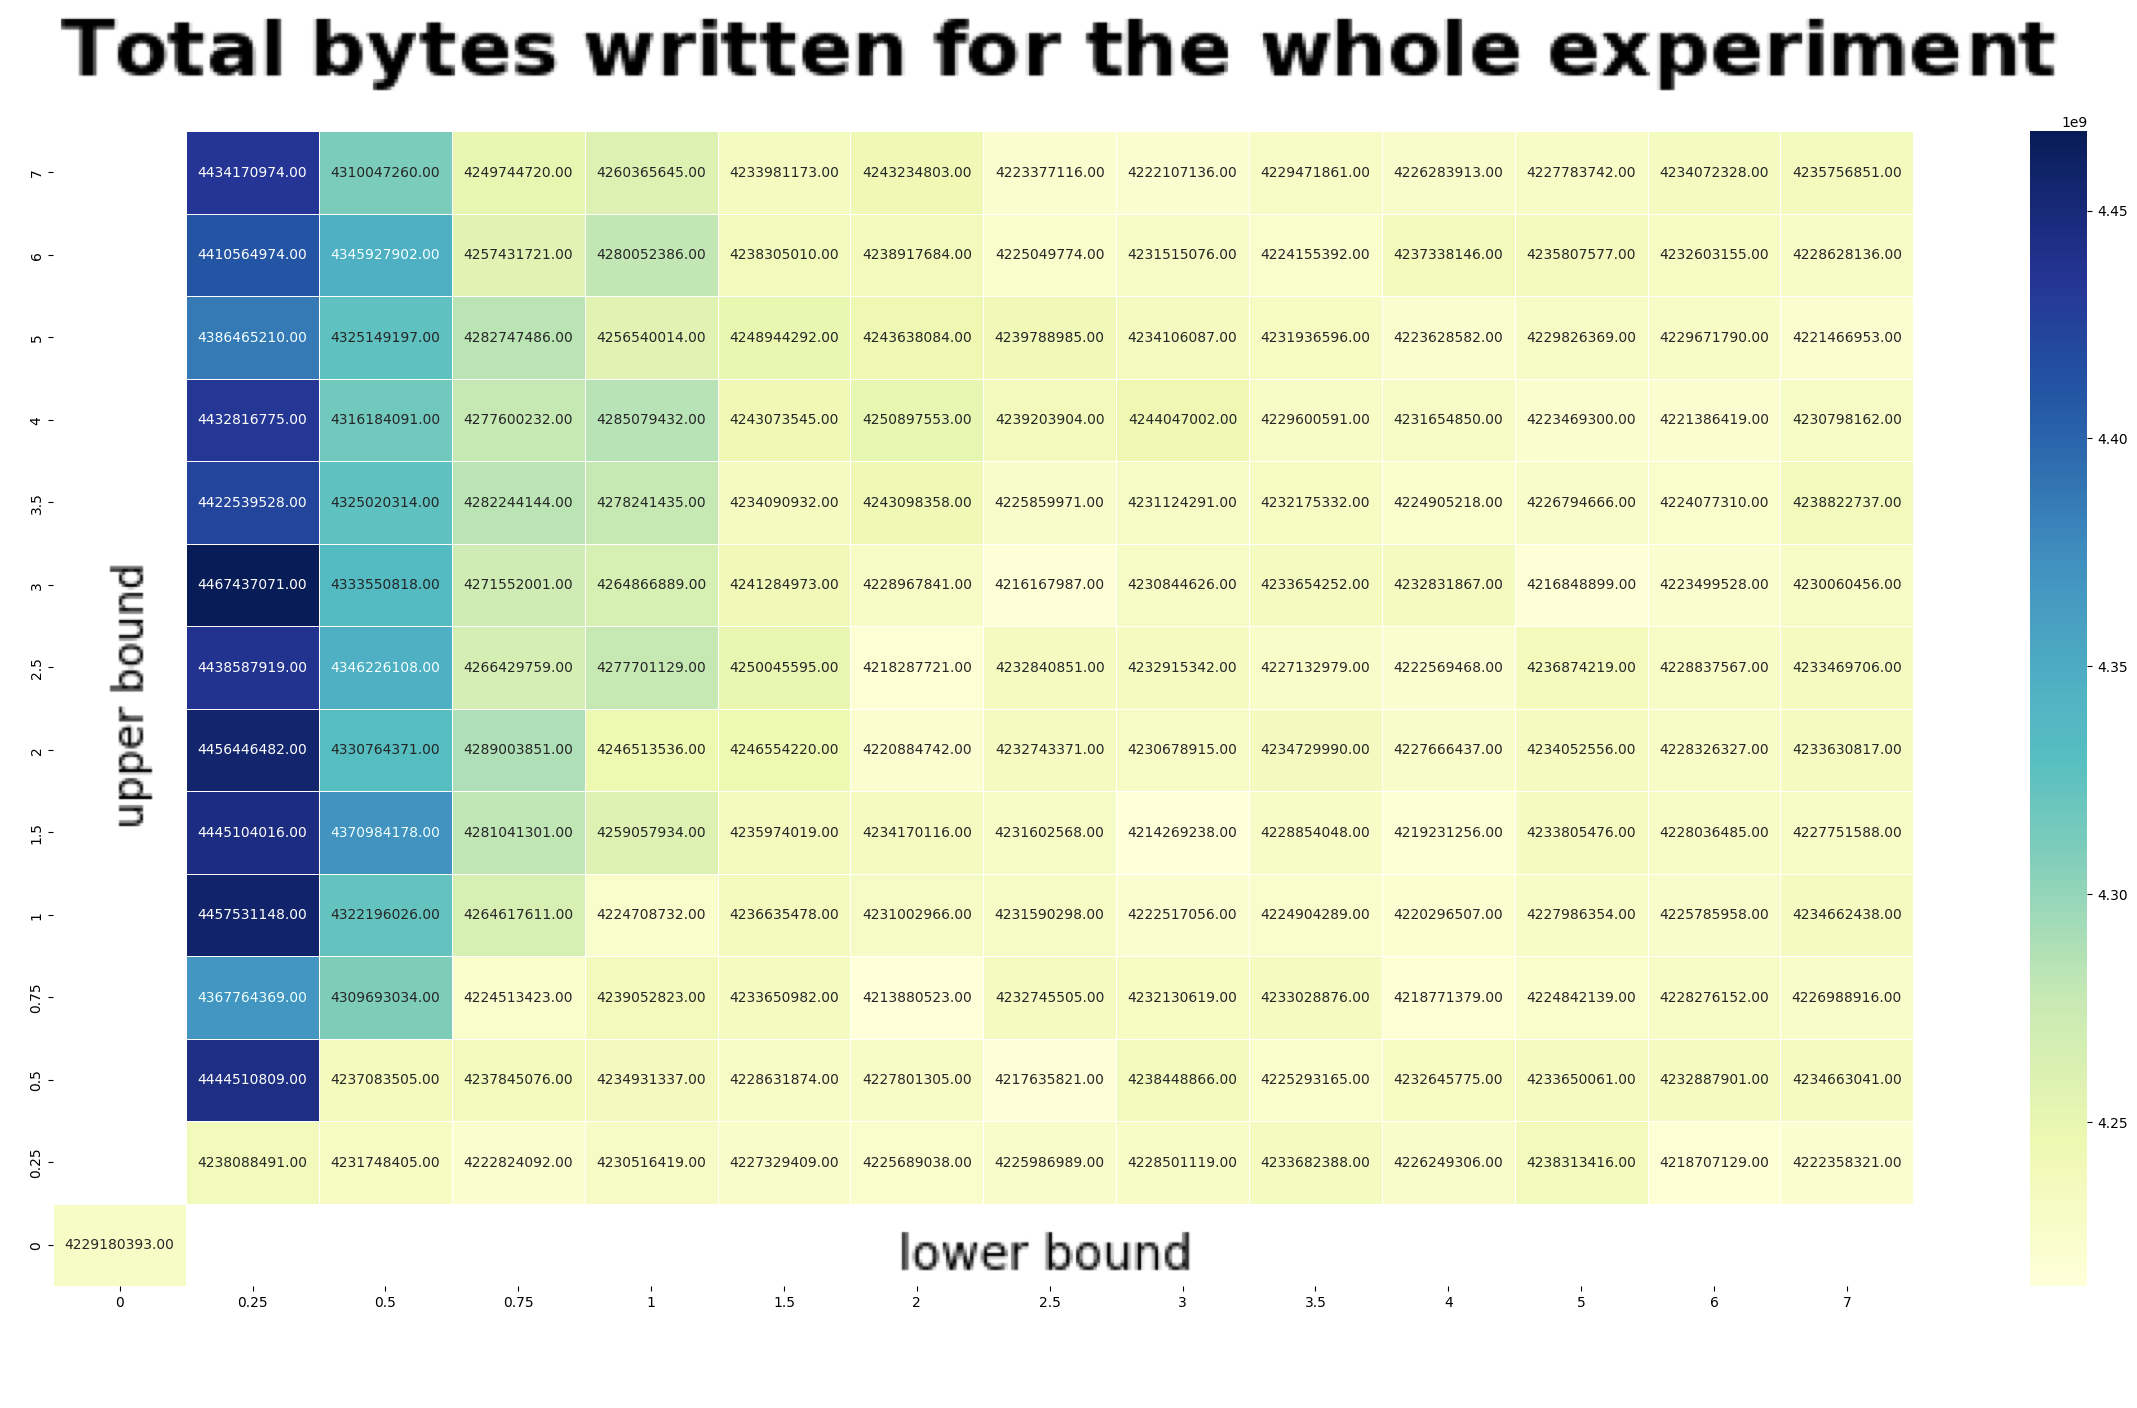
\includegraphics[width=\linewidth]{Figures/total_bytes_written.png}
    \caption{Figure shows the total number of bytes written for the execution of whole workload using different lower 
    and upper bound thresholds. The left bottom corner shows the Vanilla and rest all are for RQDC.}
\end{figure}

\begin{figure}
    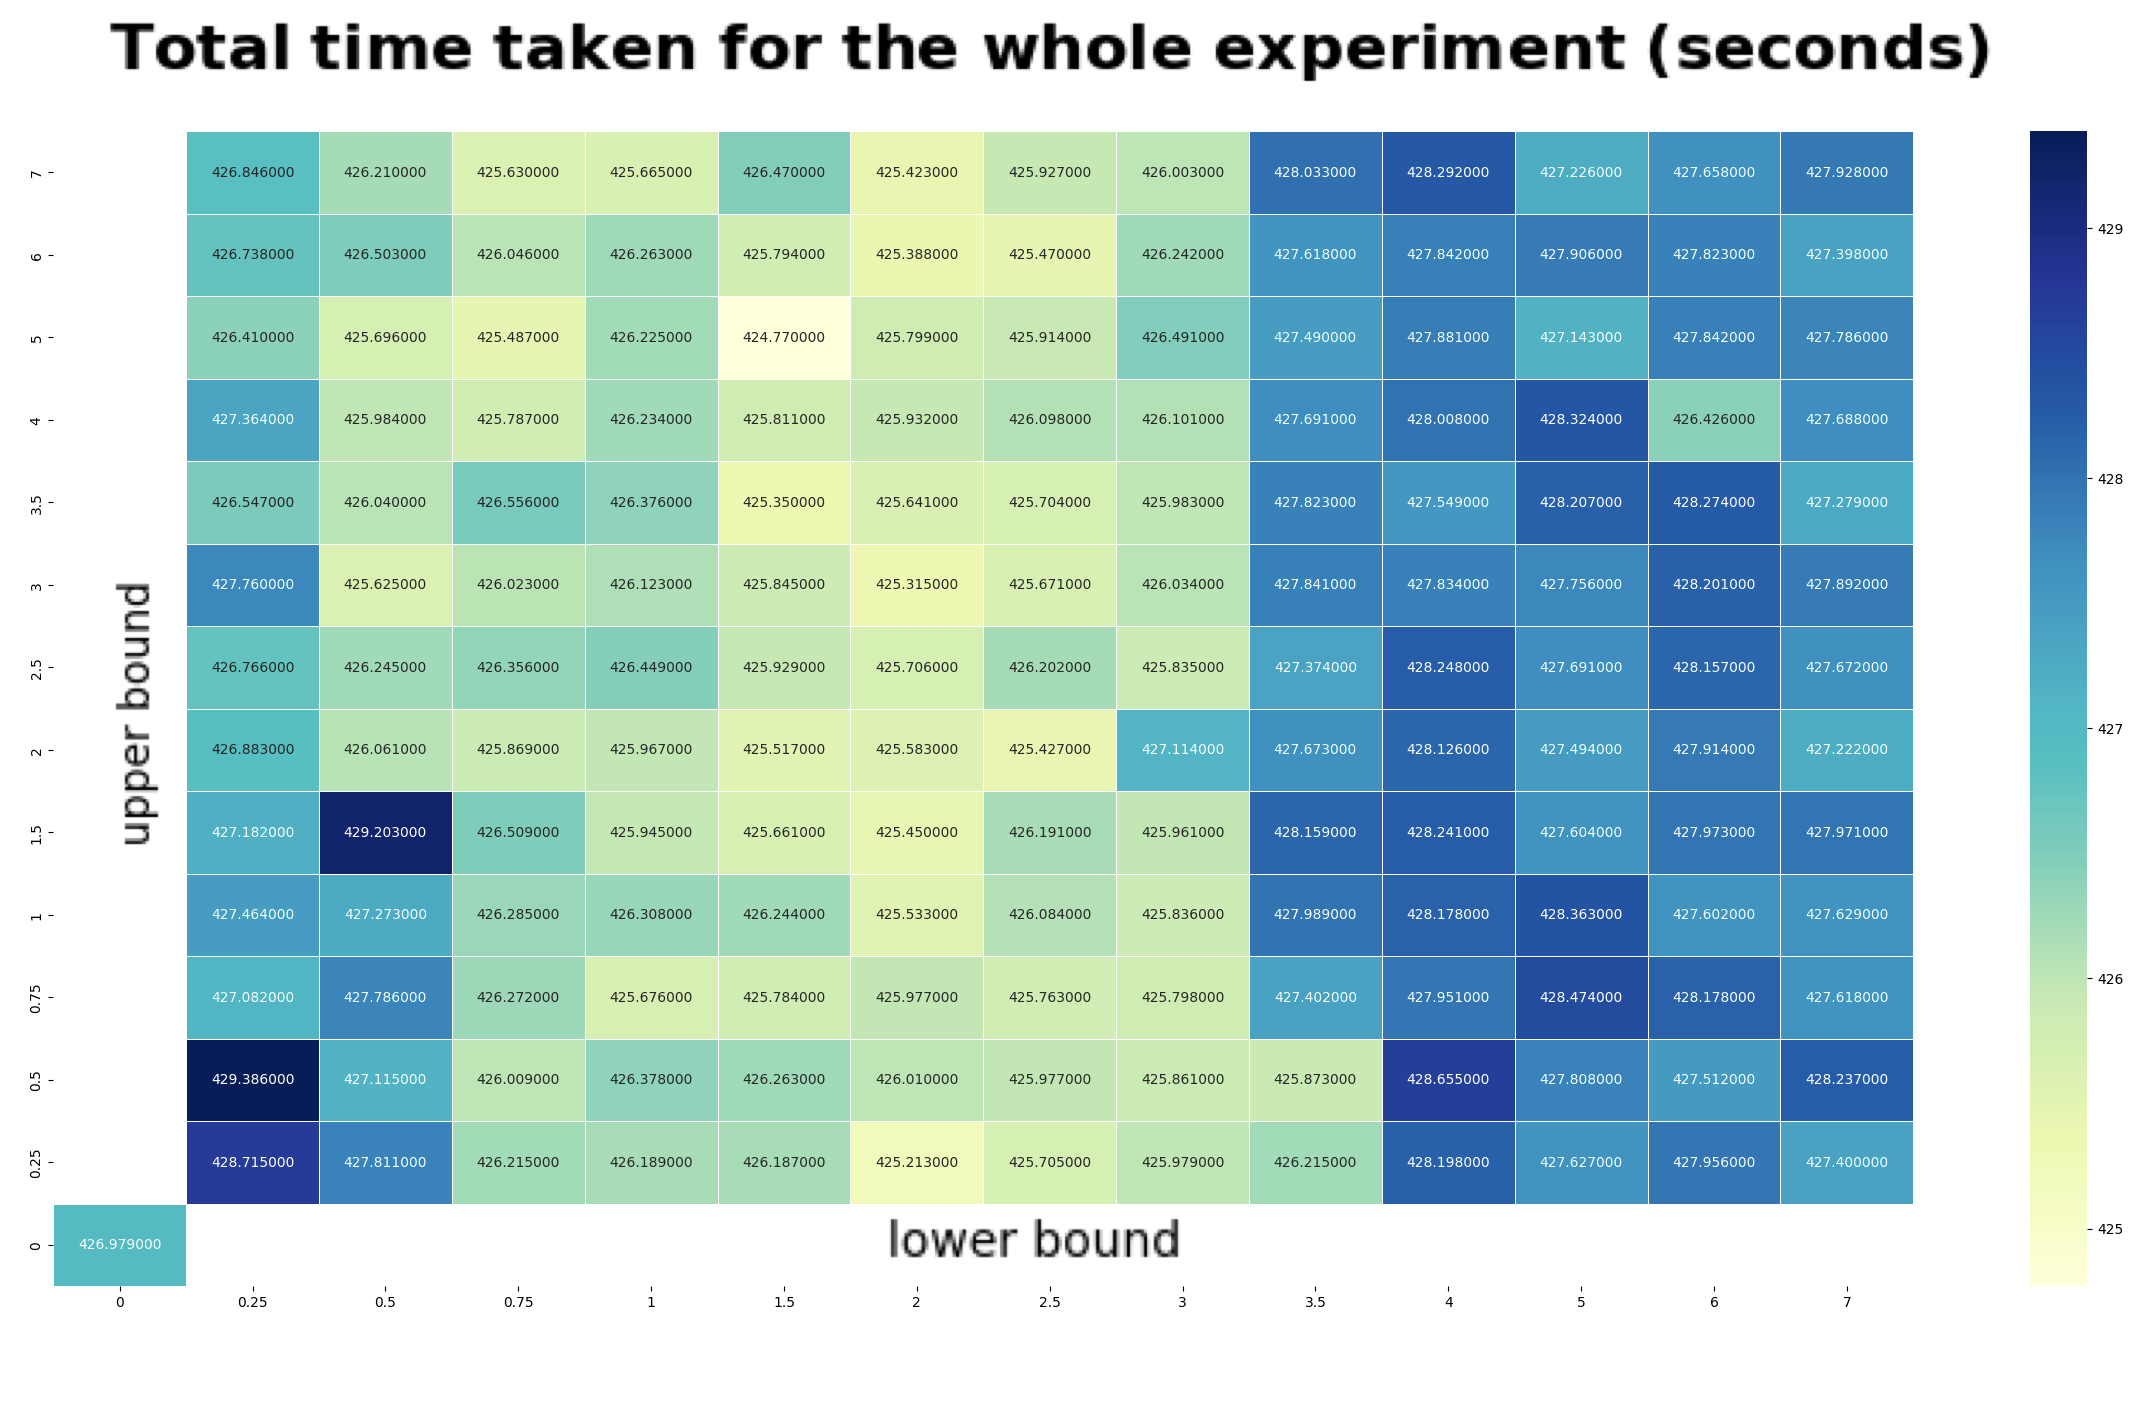
\includegraphics[width=\linewidth]{Figures/total_time_taken.png}
    \caption{Figure shows the change in workload execution time for different lower and upper bound values. The left 
    bottom corner shows the Vanilla and rest all are for RQDC.}
\end{figure}

\begin{figure}
    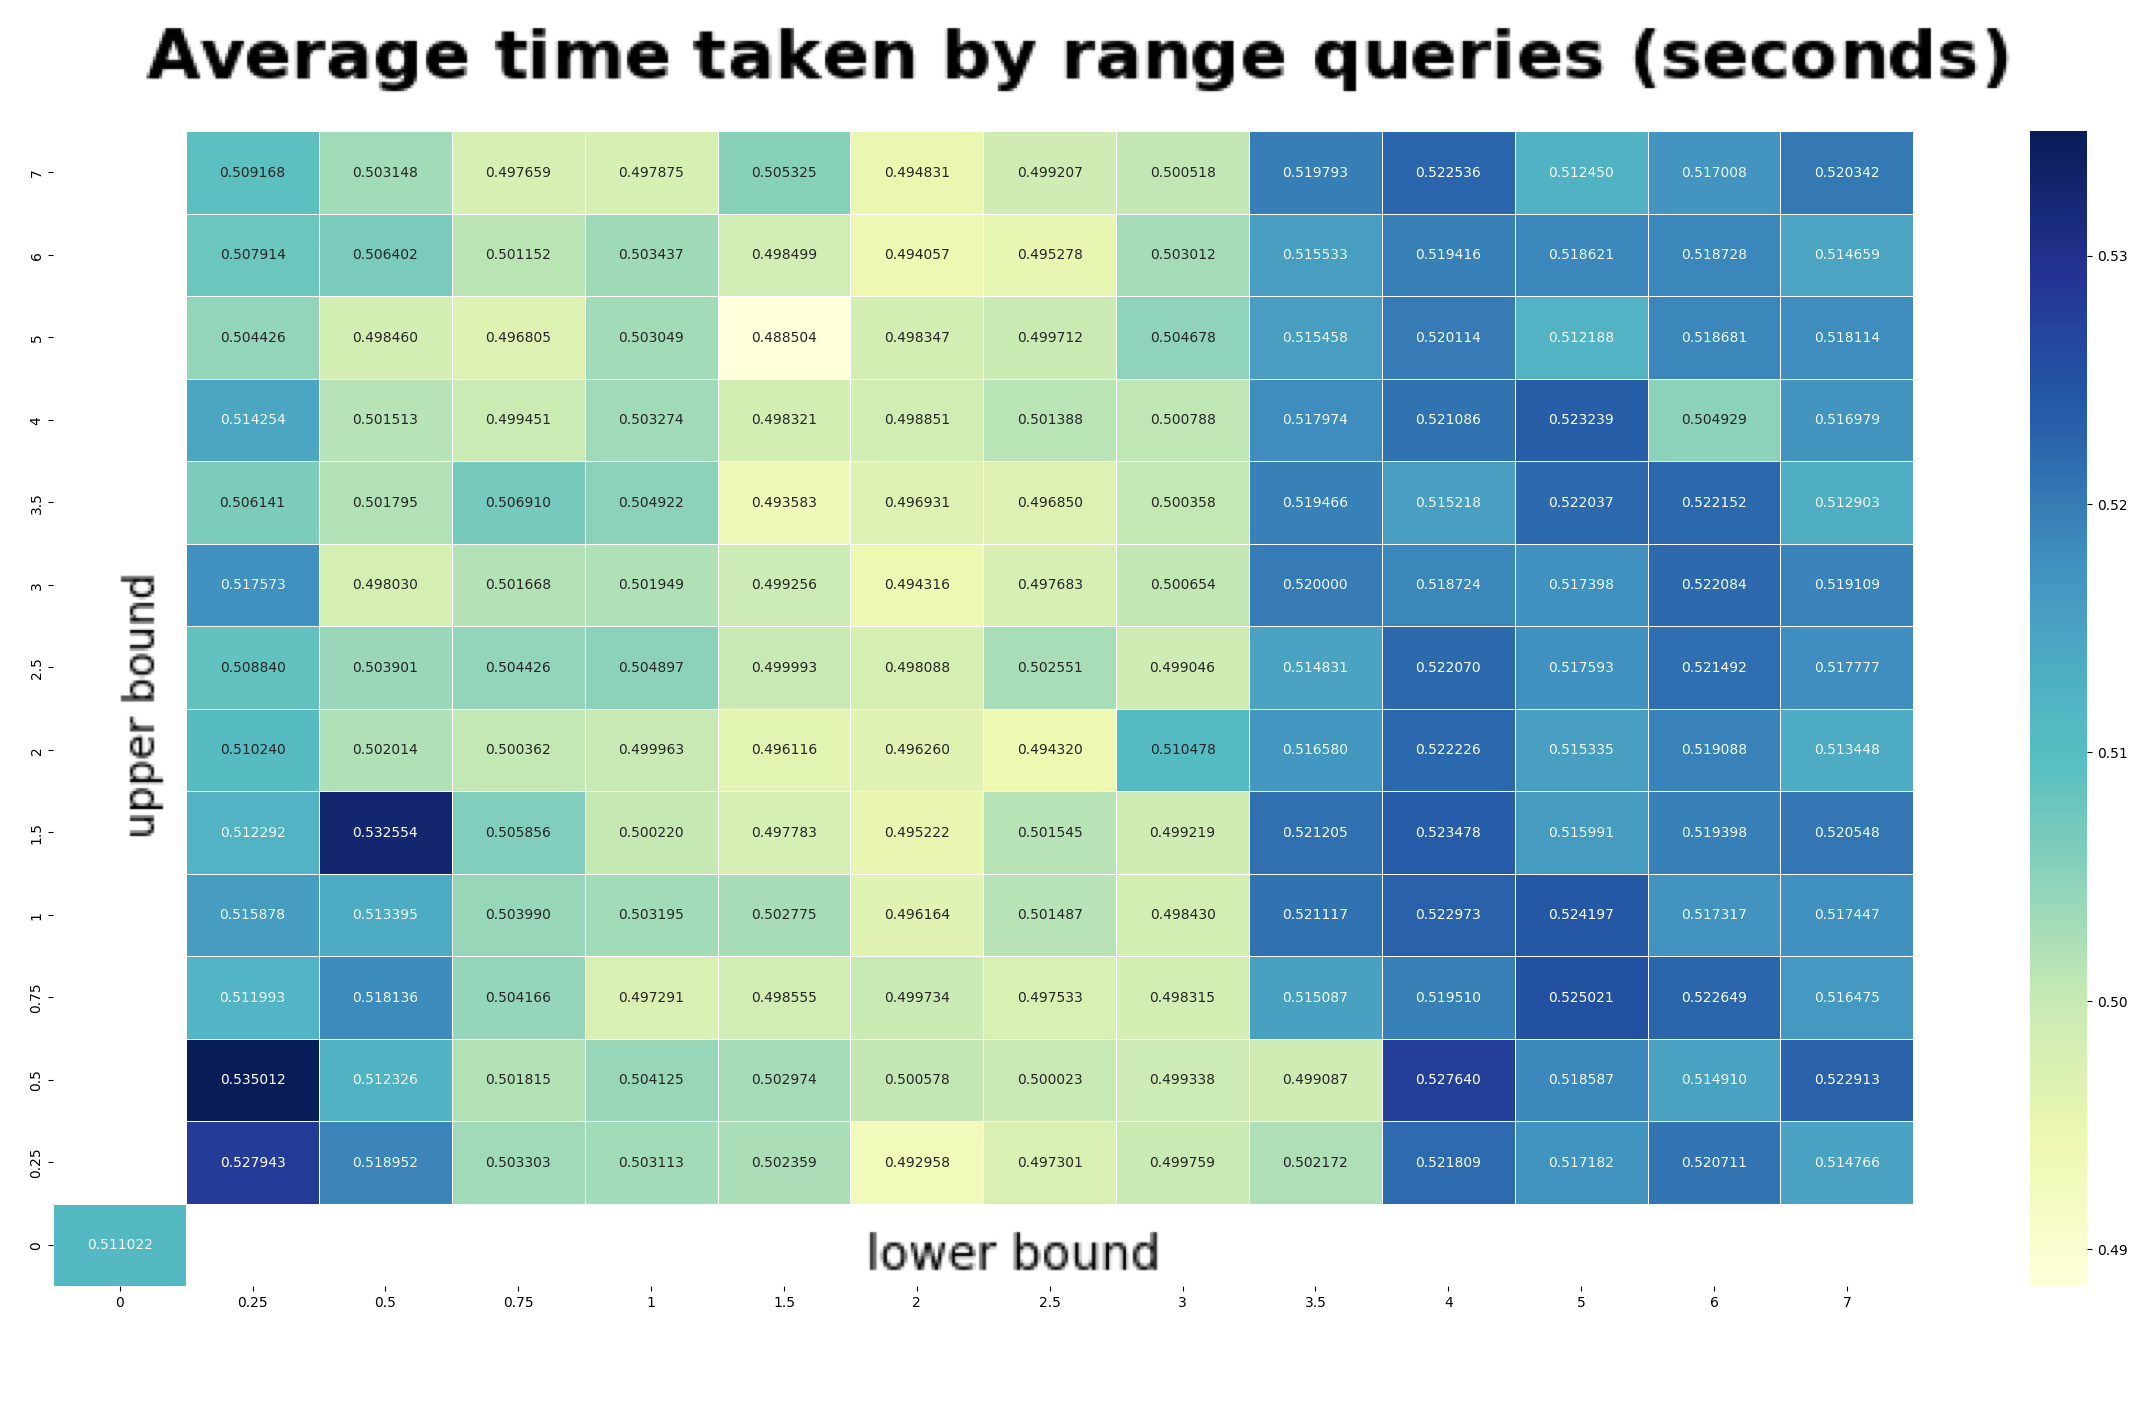
\includegraphics[width=\linewidth]{Figures/total_time_take_by_range_queries.png}
    \caption{Figure shows the change in average total time taken by range queries for different lower and upper bound 
    thresholds. The left bottom corner shows the Vanilla and rest all are for RQDC.}
\end{figure}

The results obtained thus far are highly promising, showcasing improvements in terms of space amplification, range query 
execution, and write amplification. This positive trend is particularly notable in the reduced space amplification 
coupled with enhanced range query performance, achieved with the same write amplification as the vanilla approach.

It's important to note that our experiments have primarily focused on updates. However, we anticipate that the inclusion 
of deletes, specifically in the form of point tombstones, will lead to a substantial reduction in write amplification. 
The Range Query Data Compaction (RQDC) approach, when encountering tombstones, effectively removes the corresponding 
entries from the tree, unless new updates occur after the insertion of the tombstone.

Our ongoing experiments aim to fine-tune and find more feasible values of \textit{lower\_bound} and \textit{upper\_bound}, 
recognizing that these values may vary for different size ratios and workloads. The trends observed so far, illustrated in 
Figure~\ref{fig:db_size_for_different_ub_lb} and Figure~\ref{fig:number_of_sst_files_ub_lb}, demonstrate changes in the 
size of the database with varying lower and upper bounds. Notably, the size ratio utilized in our experiments is 
randomly set at 6 \textit{(T)}.
 
\section{Conclusion}
\label{sec:conclusion}
In this study, we explored and addressed key challenges in log-structured merge (LSM) trees, particularly focusing on 
improving the efficiency of range queries and compactions in the context of write-intensive workloads. The prevalent use
of LSM trees in modern data systems prompted our investigation into optimizing the traditional approach through the 
introduction of a novel query-driven compaction strategy.

The motivation behind our work stemmed from the observation that conventional LSM designs incur redundant work and 
increased write amplification, especially when executing overlapping range queries. To tackle these issues, we proposed 
a query-driven compaction strategy that selectively removes invalid keys during range queries, significantly reducing 
the workload for subsequent queries.

Our approach demonstrated substantial benefits in experimental settings, showcasing a notable reduction in the number of 
compactions triggered during workload execution. We empirically validated the efficiency of our strategy through 
experiments conducted on a real-world LSM-based data store, RocksDB, using baremetal cloud instances. The results 
highlighted significant improvements in both speed and efficiency, particularly evident in reduced write amplification 
and optimized use of system resources.

We acknowledged the limitations of a blind application of the query-driven approach and introduced an informative 
compaction strategy to make more informed decisions based on the overlap between levels. This adaptive approach 
showcased comparable write amplification to the conventional method while providing additional advantages such as 
reduced space amplification.

The experimental findings demonstrated the effectiveness of our approach, indicating that the query-driven compaction 
outperformed traditional methods in terms of write and space amplification. Through a carefully designed experimental 
setup involving different workload scenarios and tuning parameters, we showcased the versatility and applicability of 
our strategy.

In conclusion, our research contributes to the ongoing efforts to enhance LSM-based data stores for write-intensive 
workloads. The query-driven compaction strategy, coupled with an informative decision-making approach, offers a 
practical solution to the challenges posed by overlapping range queries. Our findings provide valuable insights for 
database developers and researchers seeking to optimize the performance of LSM trees in real-world scenarios.

\section{Future Work}
\label{sec:future_work}
\begin{figure}
    \centering
    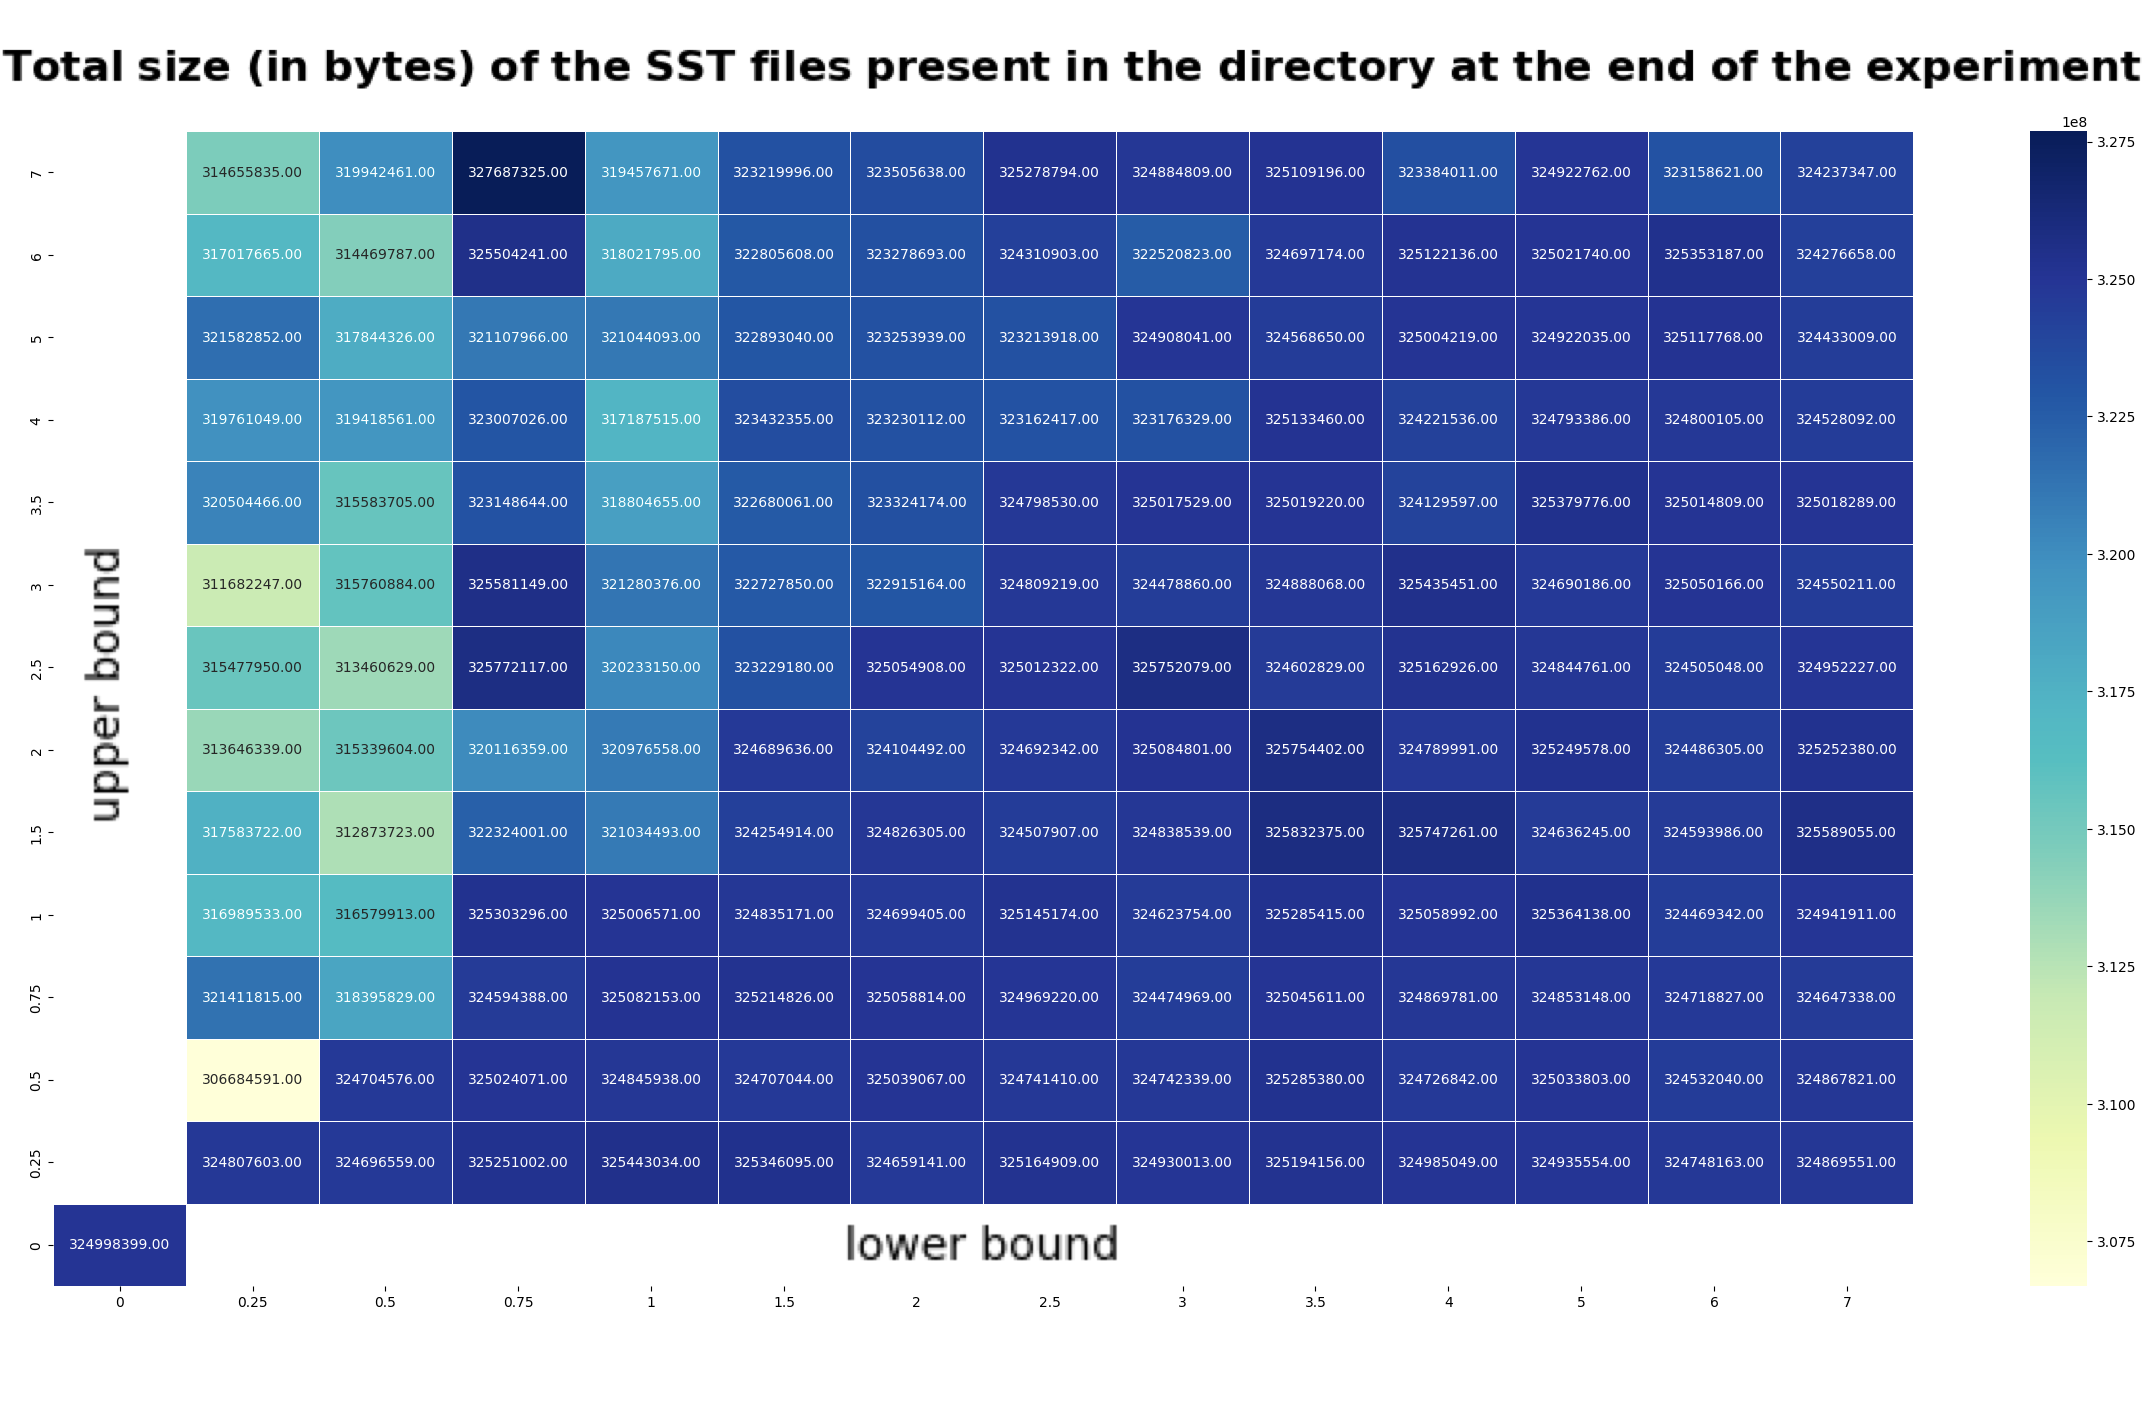
\includegraphics[width=\linewidth]{Figures/size-of-database.png}
    \caption{Figure shows how the size of database changes with different values of lower bound and upper bound.
    The horizontal axis shows the lower bound and vertical shows the upper bound. The left bottom corner shows the 
    Vanilla and rest all are for RQDC.}\label{fig:db_size_for_different_ub_lb}
\end{figure}

\begin{figure}
    \centering
    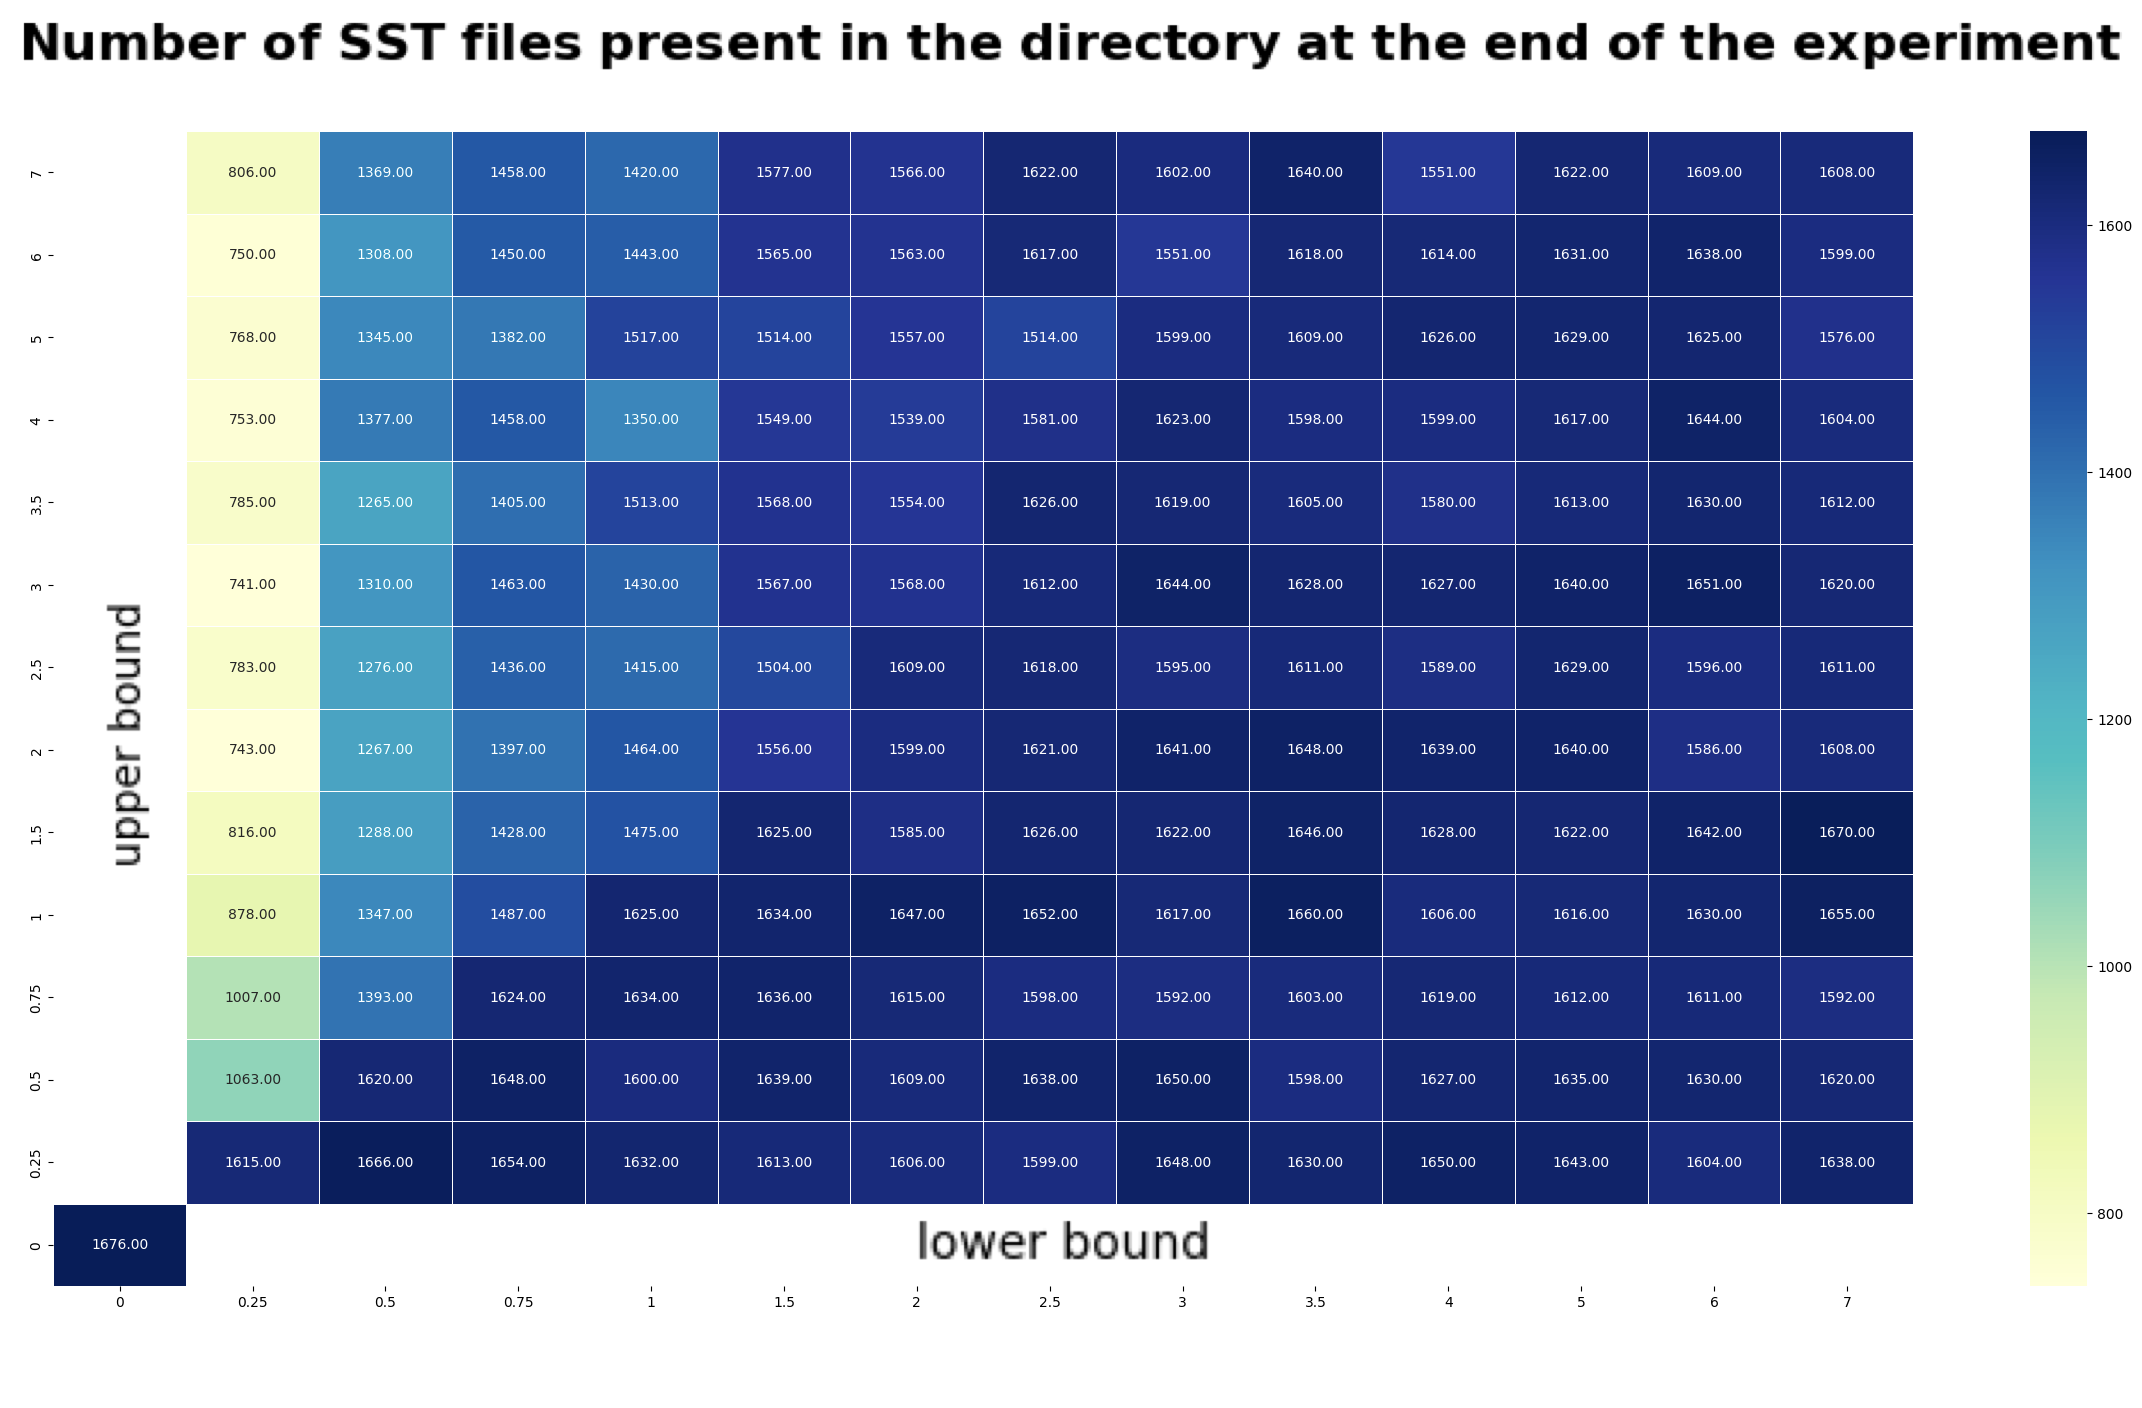
\includegraphics[width=\linewidth]{Figures/number-of-sst-files.png}
    \caption{Figure shows how the number of SST files changes with different values of lower bound and upper bound.
    The horizontal axis shows the lower bound and vertical shows the upper bound. The left bottom corner shows the 
    Vanilla and rest all are for RQDC.}\label{fig:number_of_sst_files_ub_lb}
\end{figure}

\begin{figure}
    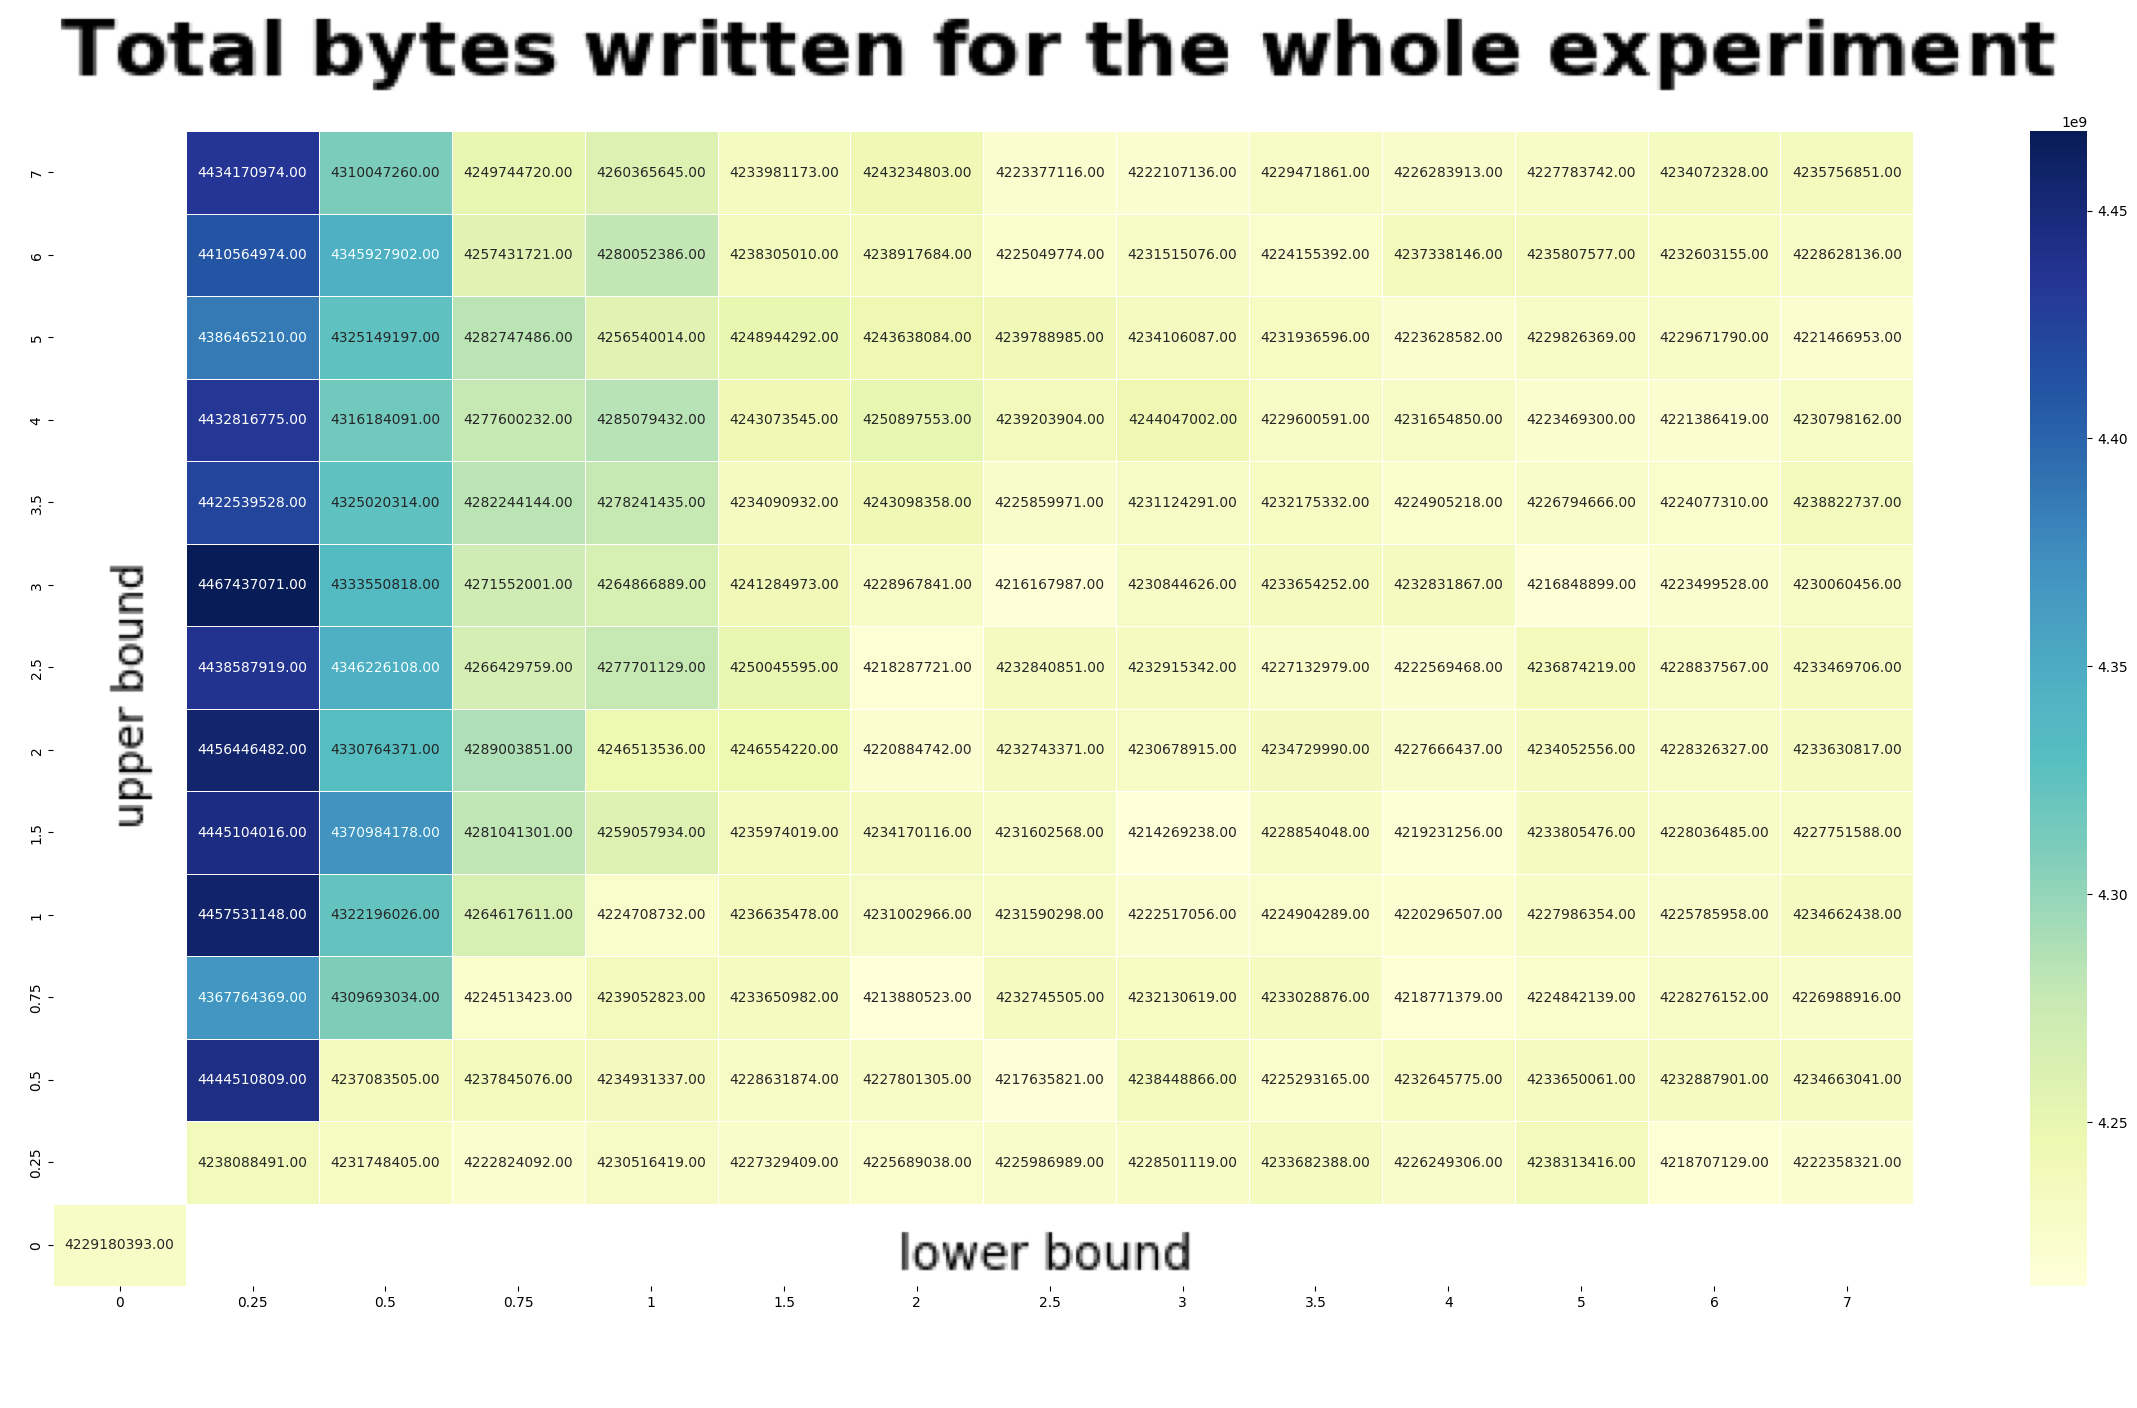
\includegraphics[width=\linewidth]{Figures/total_bytes_written.png}
    \caption{Figure shows the total number of bytes written for the execution of whole workload using different lower 
    and upper bound thresholds. The left bottom corner shows the Vanilla and rest all are for RQDC.}
\end{figure}

\begin{figure}
    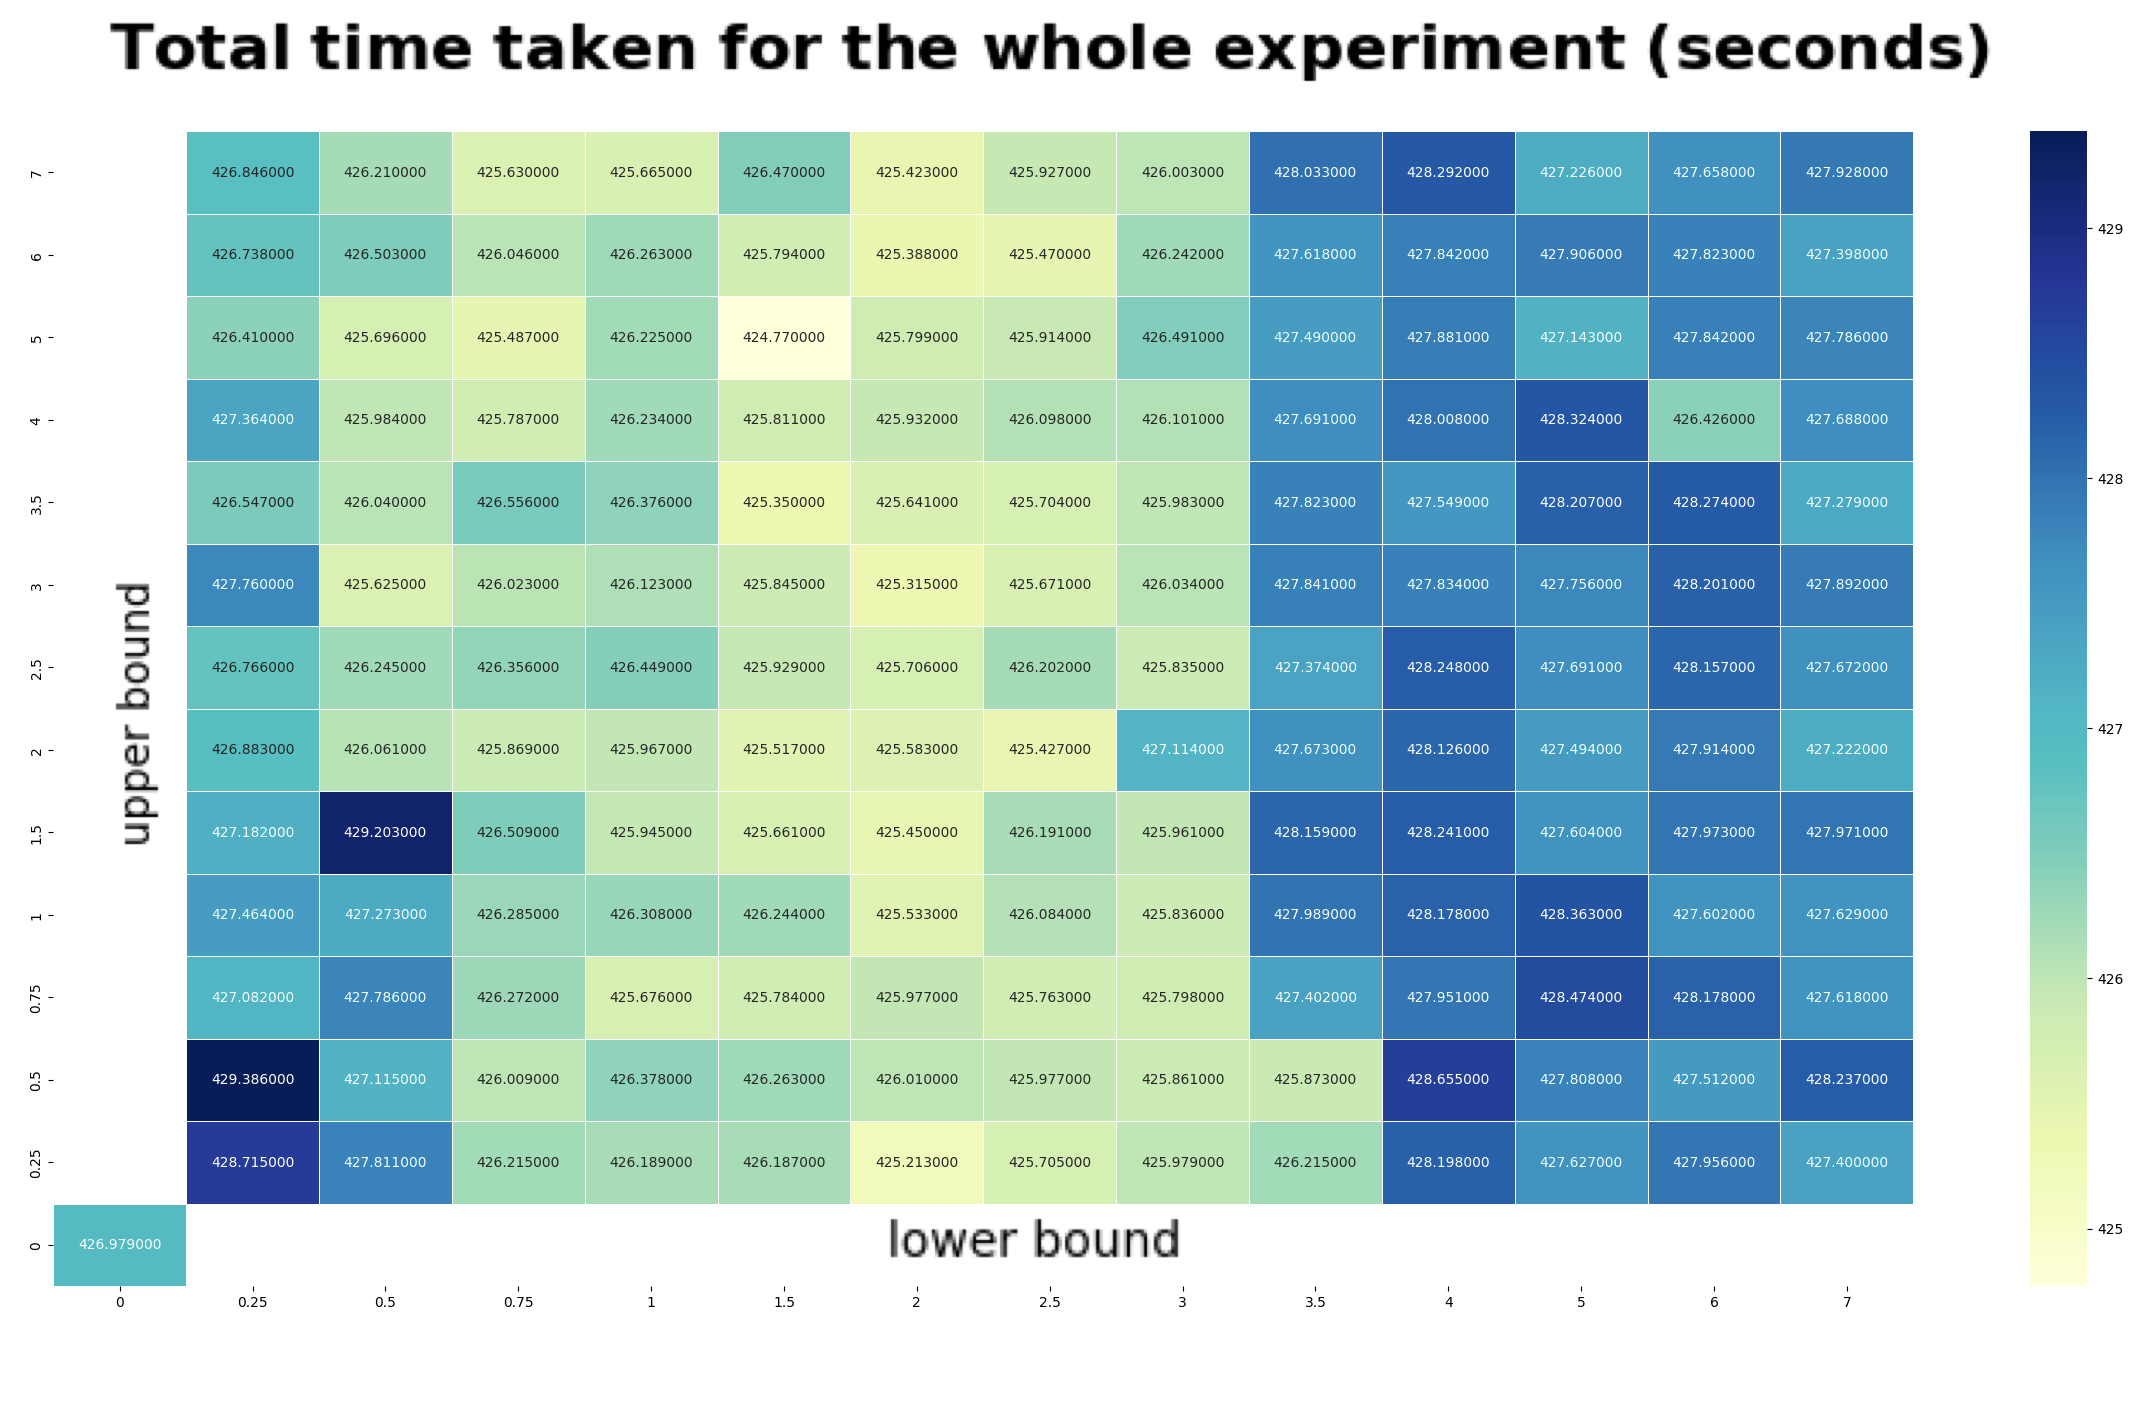
\includegraphics[width=\linewidth]{Figures/total_time_taken.png}
    \caption{Figure shows the change in workload execution time for different lower and upper bound values. The left 
    bottom corner shows the Vanilla and rest all are for RQDC.}
\end{figure}

\begin{figure}
    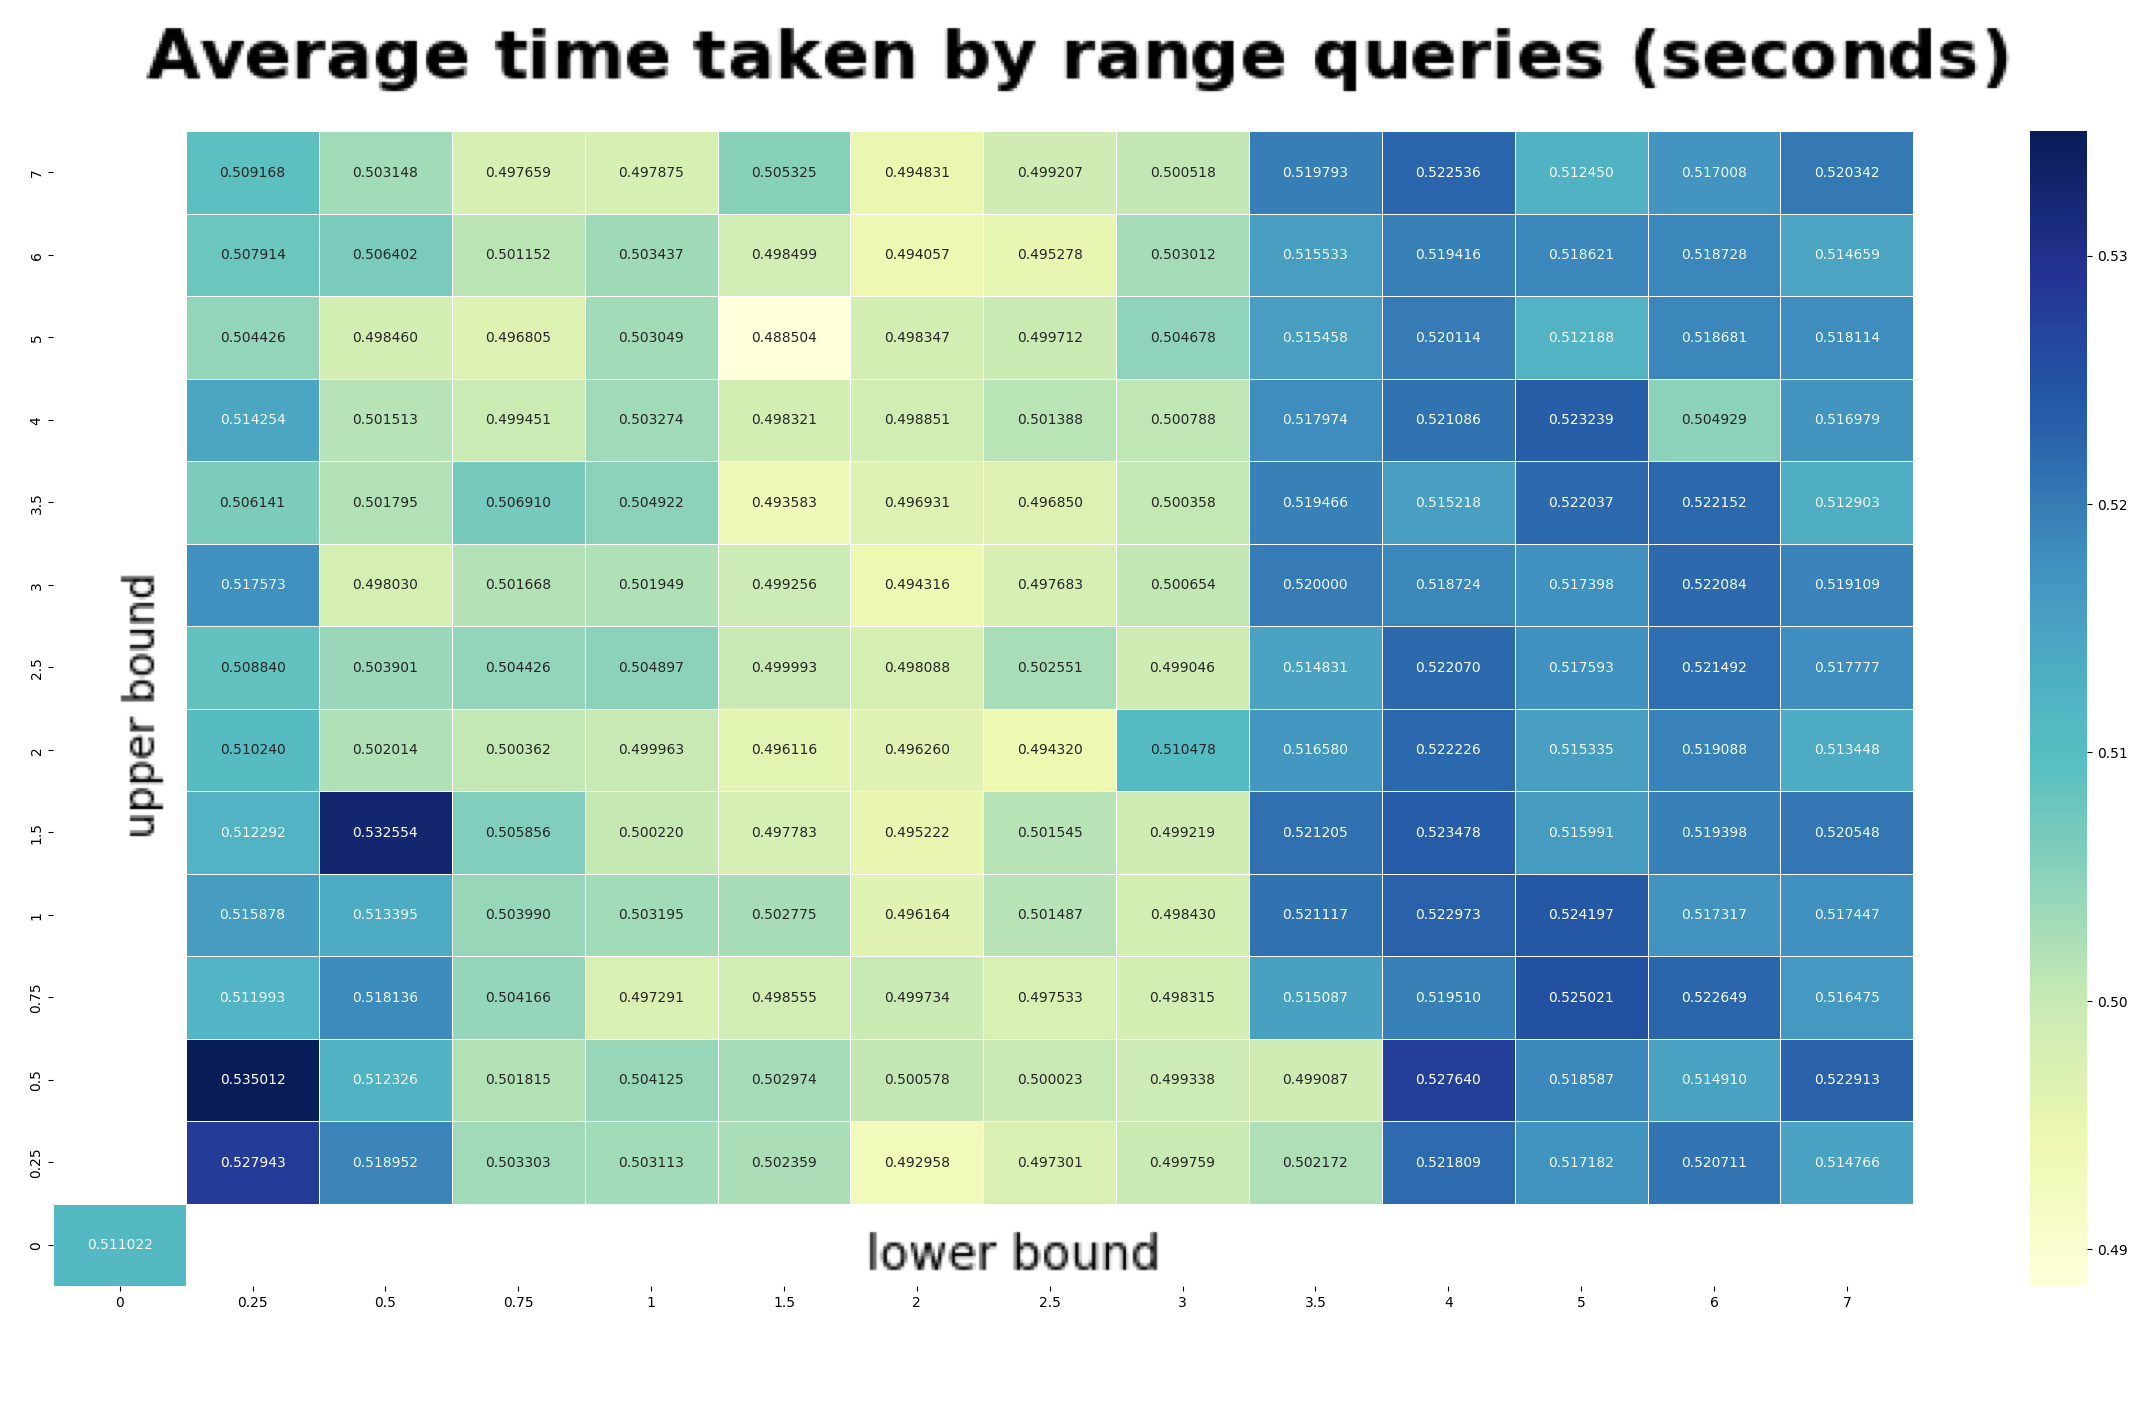
\includegraphics[width=\linewidth]{Figures/total_time_take_by_range_queries.png}
    \caption{Figure shows the change in average total time taken by range queries for different lower and upper bound 
    thresholds. The left bottom corner shows the Vanilla and rest all are for RQDC.}
\end{figure}

The results obtained thus far are highly promising, showcasing improvements in terms of space amplification, range query 
execution, and write amplification. This positive trend is particularly notable in the reduced space amplification 
coupled with enhanced range query performance, achieved with the same write amplification as the vanilla approach.

It's important to note that our experiments have primarily focused on updates. However, we anticipate that the inclusion 
of deletes, specifically in the form of point tombstones, will lead to a substantial reduction in write amplification. 
The Range Query Data Compaction (RQDC) approach, when encountering tombstones, effectively removes the corresponding 
entries from the tree, unless new updates occur after the insertion of the tombstone.

Our ongoing experiments aim to fine-tune and find more feasible values of \textit{lower\_bound} and \textit{upper\_bound}, 
recognizing that these values may vary for different size ratios and workloads. The trends observed so far, illustrated in 
Figure~\ref{fig:db_size_for_different_ub_lb} and Figure~\ref{fig:number_of_sst_files_ub_lb}, demonstrate changes in the 
size of the database with varying lower and upper bounds. Notably, the size ratio utilized in our experiments is 
randomly set at 6 \textit{(T)}.


\balance 
{
\bibliographystyle{abbrv}
% \bibliography{/Users/subhadeep/Library/CloudStorage/Dropbox/W-Lab/Bibliography-Mendeley/library.bib}
 
} 

\end{document}
\endinput

